
%: ----------------------- introduction file header -----------------------


% the code below specifies where the figures are stored
\ifpdf
    \graphicspath{{introduction/figures/PNG/}{introduction/figures/PDF/}{introduction/figures/}}
\else
    \graphicspath{{introduction/figures/EPS/}{introduction/figures/}}
\fi

% ----------------------------------------------------------------------
%: ----------------------- introduction content ----------------------- 
% ----------------------------------------------------------------------
\chapter{First Things First}
\section{Cosmic Context}\label{sec:CosmicContext}

The subject of this thesis is the ``Epoch of Reionization", also known as ``hydrogen reionization" or ``reionization" or simply the ``EoR". Let us start with a brief description of what this process is, how it relates to the evolution of the Universe as a whole, and what the open problems are regarding reionization that we are trying to solve. 


The problem of reionization arises when trying to reconcile observations of the early Universe with those of the present-day Universe. Namely, Big Bang nucleosynthesis and observations of the Cosmic Microwave Background (CMB, discussed in \S \ref{sec:CMB})\gloss{CMB}{Cosmic Microwave Background. This is the earliest available snapshot of the Universe and is composed of light which has travelled from the surface of last scattering to today, largely unimpeded.} demonstrate that, when the Universe was $\sim$380,000 years old, neutral hydrogen and helium constituted the vast majority of the baryonic matter. However, observations of nearby quasars (specifically, the \lya\ forest, discussed in \S \ref{sec:LyaForest}) demonstrate that the gas between the galaxies, dubbed the intergalactic medium (IGM)\gloss{IGM}{Intergalactic medium. This refers to the gas between galaxies, which constitutes most of the baryonic matter in the Universe.}, today is almost entirely ionized.\footnote{In \S \ref{sec:LyaForest}, we discuss how the lack of \lya\ absorption in quasar spectra is suggestive of a highly-ionized IGM. However, when this was first observed in 1965 (\citealt{1965ApJ...142.1633G}), it was not obvious that this was indicative of an \textit{ionized} IGM rather than a scenario where galaxy formation was so efficient as to remove almost all of the gas from the IGM. See \cite{meiksin2009physics} for a nice review of the physics of the IGM.} Therefore, it must be the case that some very energetic process occurred in the intervening $\sim$13 billion years which stripped the electrons from almost all of the atoms in the IGM. We refer to this process as the Epoch of Reionization.


Technically, several ionizations have to take place: ionizing hydrogen, singly ionizing helium, and doubly ionizing helium with the required energies per ionization being 13.6 eV, 24.6 eV, and 54.4 eV, respectively. Since the first two processes require similar energies, they are thought to occur concurrently. However, the complete ionization of helium requires four times as much energy as for hydrogen and likely occurs significantly later and as a result of a different process (see, e.g., \S 6.3.2 of \citealt{barkana2001beginning}). For this thesis, we focus exclusively on hydrogen ionization and the single ionization of helium and treat the term ``reionization" as being synonymous with this. 


\begin{figure}[!p]
  \centering
  \includegraphics[width=14cm]{BellUniverse.eps}
  \caption{Milestones in the evolution of the Universe from the Big Bang to today.(Photo from NASA WMAP science team)}
  \label{fig:NASAWMAP}
\end{figure}


To help understand where reionization fits into the evolution of the Universe as a whole, we can refer to Figure \ref{fig:NASAWMAP}, which shows the qualitative evolution of the Universe starting with the inflation and the CMB on the far left and ending with the present-day Universe on the right and spanning $\sim$13.8 billion years. One of the exciting aspects of reionization is that so little about it is known for sure. However, a reasonable round-number placement of reionization in this figure would be that it was an extended process that occurred somewhere between $\sim$500 million years after the Big Bang and 1 billion years after the Big Bang, likely coinciding with the formation of the first galaxies. 


The manner in which reionization progressed is also not known for sure and depends on the specifics of what energetic process is at its root. For example, if ``softer" sources, emitting ionizing radiation in the UV but not X-ray, drove reionization, then these photons will see a relatively high photoionization cross section and will not travel far before ionizing hydrogen in their path. Under this scenario, the state of the Universe during reionization would likely resemble a two-phase medium with ionized regions surrounding the ionizing sources and sharp boundaries between the ionized regions and the neutral IGM. Eventually, as the ionized regions grew, they would overlap until the entire IGM was ionized. This is the expected course for reionization in the event that it is driven by the first galaxies.	


If reionization is driven by sources with a ``harder" spectrum, emitting ionizing radiation strongly in X-ray, then the photoionization cross section of these photons will be relatively low. This is because, for photons with $E_{\gamma} \gg 13.6e\text{V}$, the cross section falls off as $\sigma \sim 1/\nu^3$. Because of this, ionizing radiation from these sources will travel \textit{farther} on average before ionizing a hydrogen atom. This will result in transitions between fully-ionized regions and fully-neutral regions being more gradual. This is the expected scenario in the case where reionization is driven by X-ray binaries or quasars. 


Additionally, \cite{McQuinn2007} investigate how the morphology of ionized regions depends on how massive the ionizing sources are. In Figure \ref{fig:McQuinnMorph}, \cite{McQuinn2007} show several reionization simulation outputs. Each panel shows the ionization field for a snapshot of a simulation. Black regions are neutral and white regions are ionized. In each row, the fraction of hydrogen atoms in the IGM that are neutral (dubbed the neutral fraction, denoted $\axhi$) is fixed and decreases for lower rows. Each column corresponds to a different mass distribution for the ionizing sources, with the masses essentially increasing as you move rightward (and assuming galaxies ionize the Universe). As such, the rightmost column demonstrates a plausible reionization scenario when very rare and massive sources dominate the ionizing photon budget. We can see this results in larger ionized regions for a fixed neutral fraction and sharper boundaries between the neutral and ionized regions. On the other hand, the left-hand columns correspond to a relatively larger contribution to the ionizing photon budget from less-massive sources. The result is a more homogeneous ionization with the ionized regions being smaller on average. Despite the uncertainties in the nature of reionization, Figure \ref{fig:McQuinnMorph} gives a qualitative picture of how reionization likely progressed: with ionized bubbles forming around sources, growing, and eventually overlapping until the effectively occupy the entire IGM. 


\begin{figure}[!p]
  \centering
  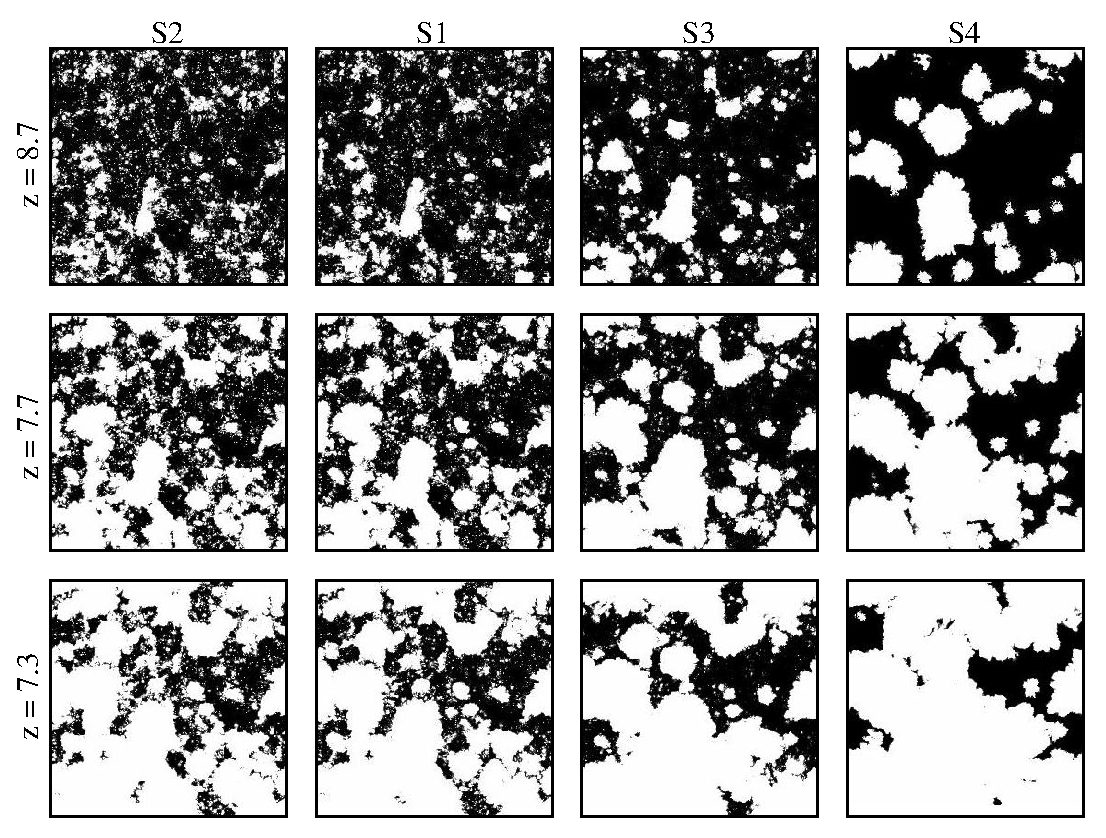
\includegraphics[width=14cm]{McQuinnHIITopology.eps}
  \caption{Simulation outputs from \cite{McQuinn2007} showing four different reionization models. Each row is at fixed $\axhi$ with $\axhi = 0.8$ (top), 0.5 (middle), 0.3 (bottom). The luminosities of the ionizing sources are related to their mass by $\dot{N} \propto m^{1/3}$ (left), $\dot{N} \propto m$ (left-middle), $\dot{N}\propto m^{5/3}$ (right-middle), and $\dot{N} \propto m$ but with a larger minimum mass (right). }
  \label{fig:McQuinnMorph}
\end{figure}


With this qualitative picture in mind, it may be worth emphasizing why astrophysicists and cosmologists care about reionization in the first place. First, the Epoch of Reionization is a significant missing piece in the story of the evolution of the Universe and represents a period in the history of the Universe where we have very few direct observations. Work towards understanding reionization is in line with the overarching goal of pushing observations further and further back in time. Second, the Epoch of Reionization marks the time when radiation from luminous sources became the dominant influence on the IGM and understanding the source of this radiation is interesting in its own right. Understanding the evolution in the properties and number of these bright sources is essential for complete cosmological models. Additionally, while the best guess for the source of the ionizing radiation is dwarf galaxies, it is possible that reionization studies will reveal more exotic and unexpected scenarios, such as annihilating dark matter playing a significant role. Third, the temperature and ionization state of the gas in the Universe plays a regulatory role in galaxy formation: hot and ionized gas will take longer to cool and collapse than cold neutral gas. Since reionization significantly affects both the temperature and ionization state of the gas, understanding reionization will be essential for understanding subsequent galaxy formation. 


Toward these goals, astrophysicists and cosmologists are striving for a thorough understanding of the timing and nature of reionization. When did it happen? How long did it take? What were the ionizing sources? What were the properties of the ionized regions and how did they evolve? These are the questions we should keep in mind throughout the rest of this thesis.

\clearpage
\subsection{Simulations}

In this thesis, we aim to develop measurements that can be applied to existing and future data sets in order to constrain the process of reionization.  In order to do this, we utilize simulations of the Universe at different times and assuming different cosmological and astrophysical parameters. We then process the simulation outputs according to the details of specific experiments in order to generate plausible mock observations from those experiments. While I perform this processing, the simulations used are not my own and the exact simulation used depends on the problem at hand. Within each subsequent chapter, we will describe the details of the simulations used, but let us give a brief overview up front.


When considering filtering techniques and the 21-cm line (discussed in \S \ref{sec:21cm}, \ref{sec:Bubble}), we generate mock observations for interferometers, which have large fields of view. Furthermore, we care about properties of the IGM on large scales, $\gtrsim$ 10\mpch, and are comfortable with sacrificing some precision on small scales. As such, we utilize large simulations with a $1 (\text{Gpc}/h)^{3}$ volume, according to a prescription described in \cite{Zahn2006}. In this case, a realization of the linear density field is generated and each dark matter halo satisfying $M_{\text{halo}} > M_{\text{min}} = 10^{8}M_{\odot}$ is given an ionizing source with ionizing emissivity proportional to $M_{\text{halo}}$. Each source is assumed to have a fixed ionizing efficiency at each time step of the simulation.  To generate the ionization field at a given time step, an excursion-set-formalism approach is used. To do this, the simulation is smoothed with progressively smaller spheres and if, at any point, the ionizing radiation contained within a sphere centered on some pixel is sufficient to ionize the number of hydrogen atoms within that sphere, the pixel is marked as ionized. The precise ionization efficiency can be adjusted in order to obtain a desired neutral fraction. This approach has the advantage that it is significantly faster than full radiative transfer calculations and is accurate at the scales of interest. 


When considering stacking techniques (described in \S \ref{sec:NeutralIslands}) aimed at detecting the HI damping wing (described in \S \ref{sec:IntroDampingWing}) and deuterium, we are interested in the IGM on smaller scales. Additionally, we are generating mock \lya\ forest observations which are one-dimensional and span smaller distance scales than for the 21-cm observations. This motivates us to use smaller simulation volumes with more accurate physics at the small scales. Specifically, we use simulated density and ionization fields generated from a dark-matter-only simulation of \cite{McQuinn:2007dy} which tracks $1024^{3}$ dark matter particles in a simulation cube with sidelength $L = 130\mpch$. In this case, the ionization field is calculated by casting rays from each ionizing source, assuming ionizing sources have a soft UV spectrum. The temperature field is obtained through a modified temperature-density relation (Eq. \ref{eq:TDrelation}).


When considering measurements of the thermal properties of the post-EoR IGM, we use two types of simulations. The first set of simulations is the same as for the stacking approach, except we assume a fully-ionized IGM. In this case, though, the previously-mentioned excursion set formalism is applied in order to identify the redshift at which each pixel ionizes. This is necessary since the temperature of a gas parcel depends on how much time has passed since photoionization, which varies spatially. Additionally, smoothed-particle hydrodynamic simulations from \cite{Lidz2010} are used in order to more closely capture the gas properties and their evolution after reionization. 

\section{The Shoulders of Giants} \label{sec:Probes}

Before we continue, it is first worth appreciating the difficulty of what we are trying to do. Essentially, we care about measuring the properties of the intergalactic gas -- not stars or galaxies -- when the Universe was only $\lesssim$1 billion years old, a seemingly impossible task. Fortunately, we are given the invaluable gift that light travels at a finite speed and, as such, if we look at distant objects, we see them as they were in the past. Therefore, if we look at the at the gas between galaxies $\sim$13 billion light years away from us, we will see it as it was roughly 13 billion years ago, when the Universe was only 1 billion years old. This means that, in principle, this information of how the young IGM evolved is directly available to us. However, even taking this into account, the intergalactic gas we care about is not bright and it is located extremely far away, so how are we supposed to observe it? An inspiring aspect of studying the Epoch of Reionization is that, when confronted with such a seemingly impossible task, experts in the field have developed many different creative approaches toward constraining the properties of the young IGM. It is this impressive body of work that we aim to build upon. We discuss a selection of the existing and future methods for constraining the EoR in this chapter in order to provide some context and motivation for our work. 

\subsection{The \lya\ Forest}\label{sec:LyaForest}
Arguably the most powerful tool for constraining the high-redshift IGM to date has been the \lya\ forest\nomenclature[Zp]{\lya\ Forest}{This describes the pattern of absorption lines seen blueward of the rest-frame \lya\ line, typically in quasar spectra. These absorption lines can be due to significantly neutral gas in the diffuse IGM or due to dense ionized gas.}. This refers to the pattern of absorption lines seen in the spectra of distant bright objects due to intervening hydrogen, as we will discuss. The \lya\ forest results, in part, from another invaluable gift to the field of cosmology: the redshifting of light with the expansion of the Universe. As the Universe expands, space itself expands and with it the wavelengths of photons travelling through it expand as well. If we know the expansion history of the Universe, and know the intrinsic color of a luminous object, then we can use its \textit{observed} color to determine our distance to the object. Because of this relationship, distances to objects are often measured as a redshift\nomenclature[Zp]{Redshift}{A quantity commonly used to refer to cosmic periods of time or distances. The redshift of an object or location in space is defined as the fractional increase in wavelength that a photon undergoes due to the expansion of the Universe while travelling from the object or location to us.}, defined as the fractional increase in wavelength that a photon experiences when travelling from a given distance to us, denoted by $z$ and defined according to the expression: 

\begin{align}
\lambda_{\text{observed}} &= \lambda_{\text{emitted}}(1+z_{\text{emitter}}). 
\end{align}

The \lya\ forest is seen in the spectrum of extremely bright background objects, usually quasars \gloss{Quasar}{Quasars are extremely bright sources of radiation associated with the accretion disk of a super-massive black hole. The emission from a quasar is beamed in a direction perpendicular to the accretion disk.} or gamma-ray bursts (GRBs)\nomenclature[Zp]{GRB}{Gamma-Ray Bursts are short-lived, yet extremely energetic, bursts of gamma rays. The initial burst can last from milliseconds to several hours. They are the most energetic events known to occur in the Universe.}, after their light has been processed by the intervening gas. Since the intervening gas is primarily composed of hydrogen and since this hydrogen is generally in the ground state, any intervening neutral patches will absorb light from the background object at the Lyman-series\gloss{Lyman Series}{The series of transitions in an atom where an electron is transitioning to or from the ground state.}wavelengths, with the strongest absorption occurring at the \lya\ wavelength: $\lambda_{\alpha} \approx 1216$\AA. If the Universe were not expanding, then all intervening neutral hydrogen would absorb light from the quasar at one wavelength: $\lambda_{\alpha} \approx 1216$\angstrom, neglecting the other lines in the Lyman-series for the moment. However, due to the expansion of the Universe, photons emitted from the quasar/GRB \textit{blueward} of the \lya\ line will redshift as they travel towards us. If they encounter neutral hydrogen as they redshift through the \lya\ line, then they will be absorbed and an absorption line will be seen in the spectrum of the background quasar at a wavelength \textit{blueward} of \lya\ (in the rest frame of the quasar/GRB). This process is sketched in Figure \ref{fig:LyaCartoon}. Thus, the \lya\ forest is the pattern of absorption lines seen blueward of the rest-frame \lya\ line in quasar spectra due to intervening neutral gas. 

\begin{figure}[!p]
  \centering
  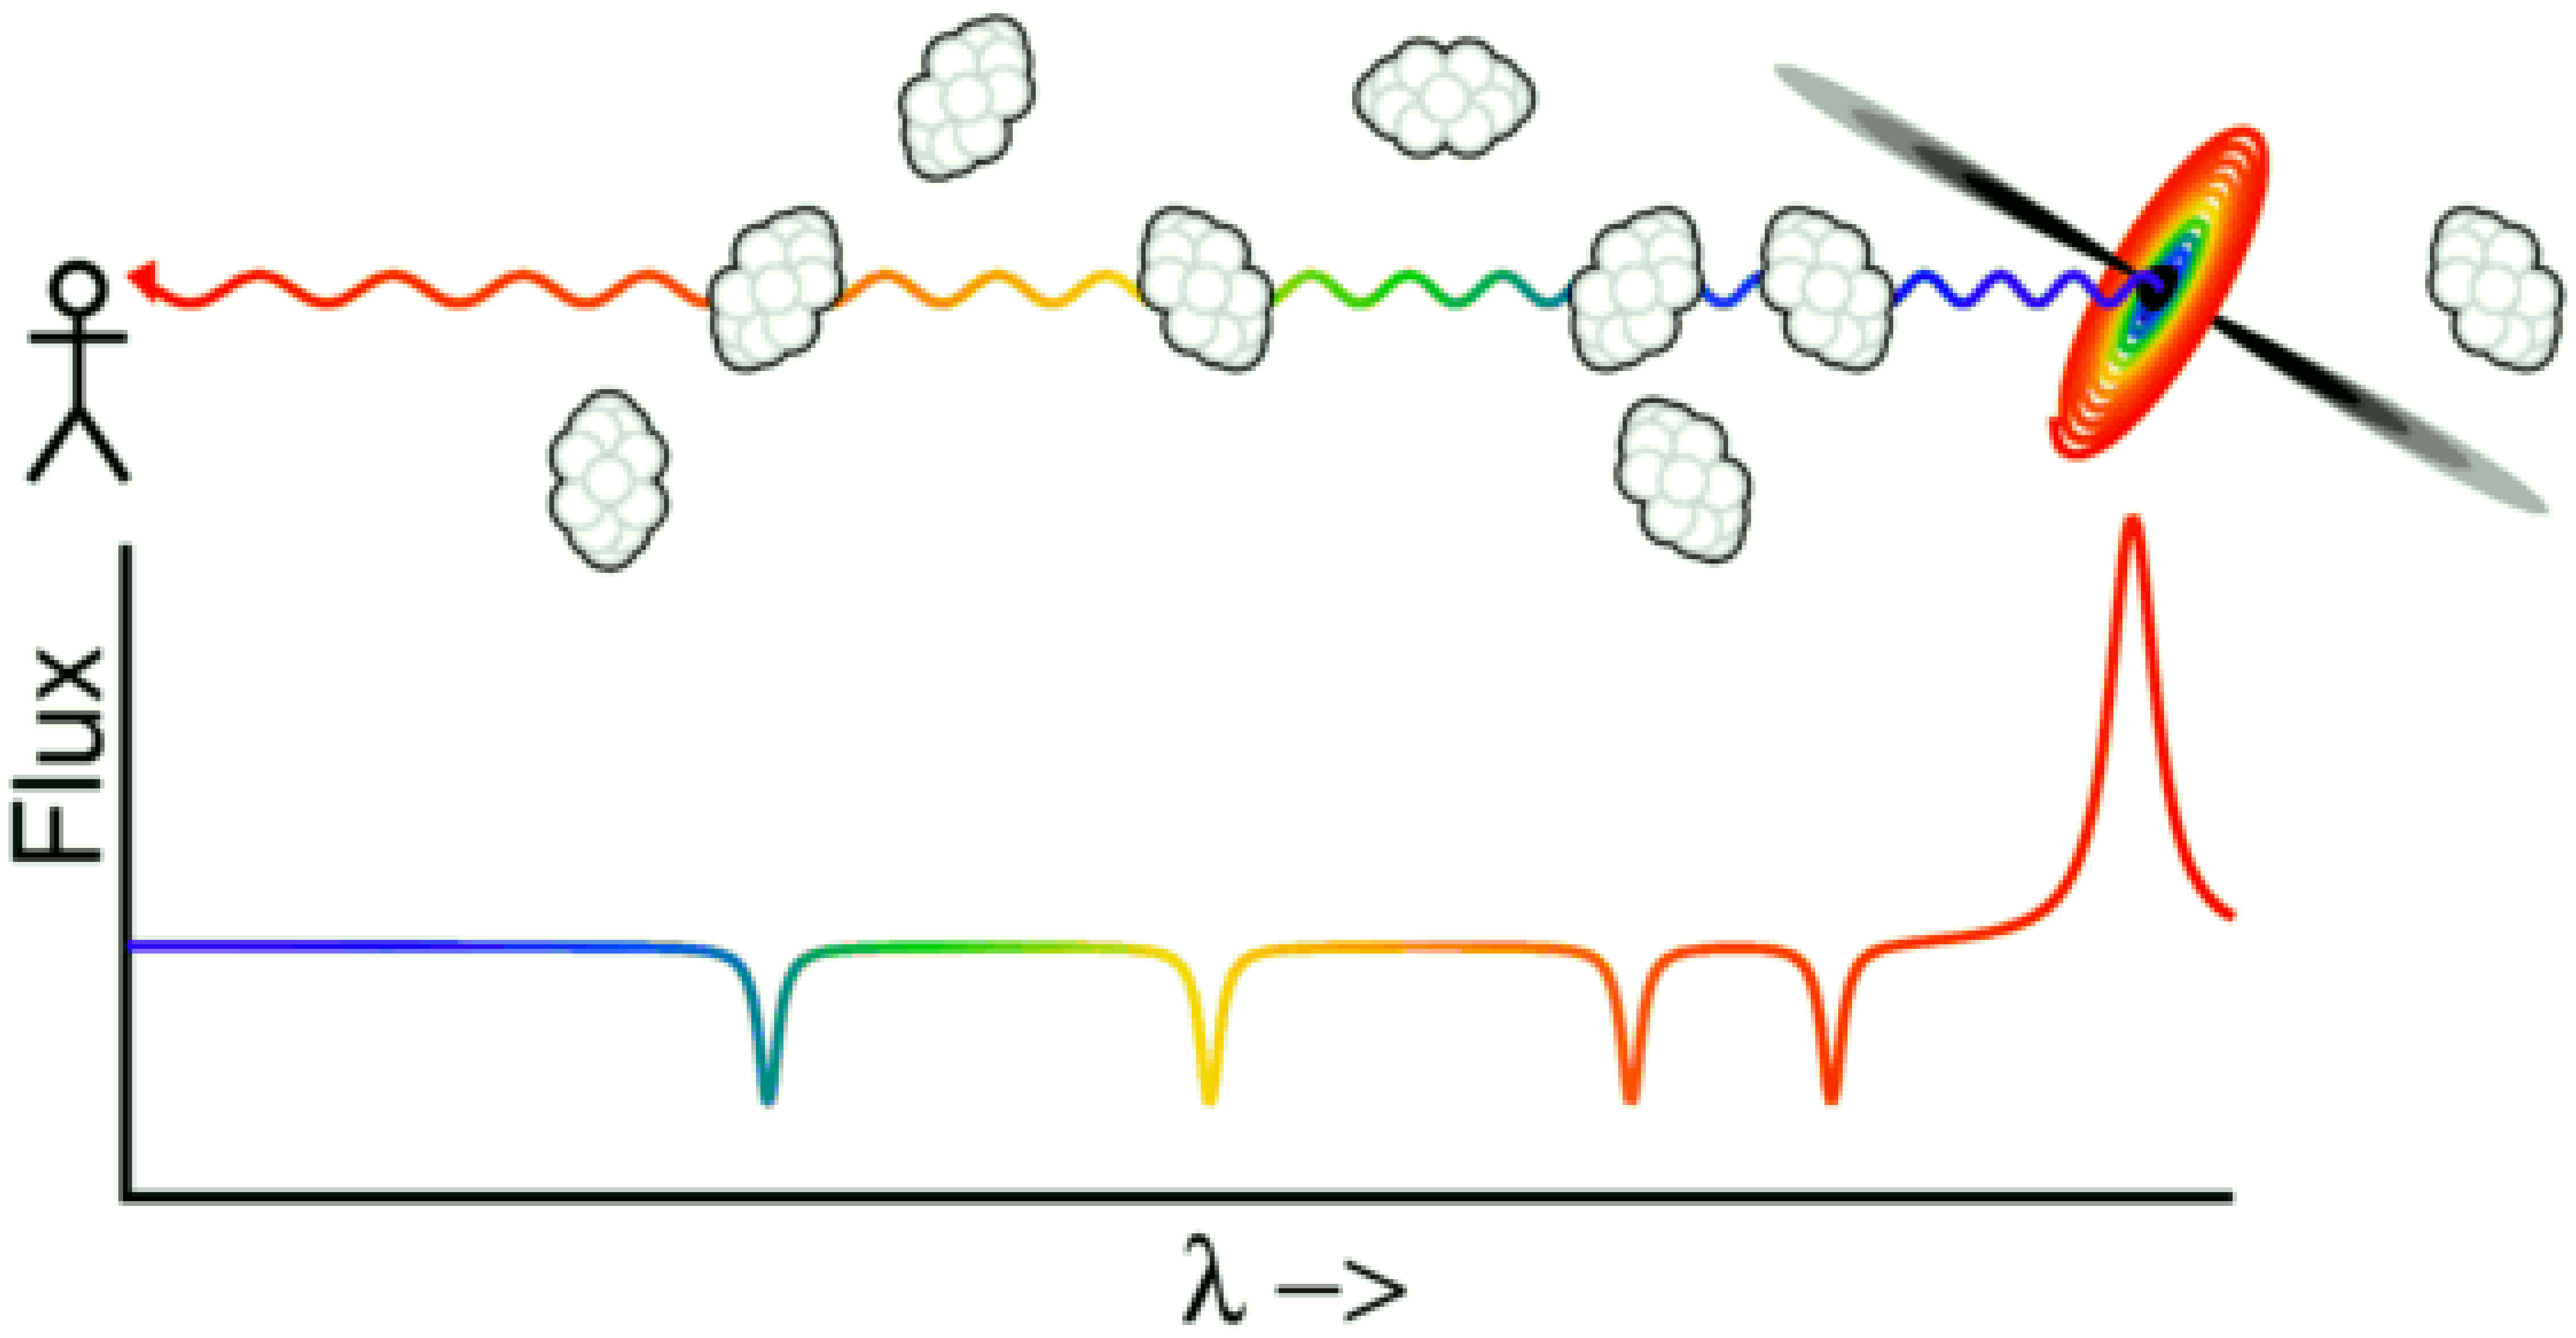
\includegraphics[width=12cm]{lyaf-75.eps}
  \caption{Illustration of the basic physics behind the \lya\ forest and how gas at different locations along the line of sight results in absorption lines at different wavelengths. (Image from {\tt http://www.astro.ucla.edu/})}
  \label{fig:LyaCartoon}
\end{figure}

The same logical progression also applies to the other lines in the Lyman-series. Therefore, you could imagine observing a \lyb\ and Ly\ $\gamma$\ forest at smaller wavelengths. There are a couple differences, however. First, lines deeper in the series have a smaller cross section for absorption, so intervening hydrogen will absorb less at these frequencies. Second, photons emitted from a background source with energies larger than \lyb\ will redshift through the \lyb\ wavelength and \textit{also} possibly through the \lya\ wavelength before reaching us and will have two opportunities to be absorbed. The photon's physical location when it redshifts through those two wavelengths will be completely different and, therefore, when observing absorption lines in the \lyb\ forest, it can be difficult to tell if the photons were absorbed by distant gas undergoing a \lyb\ transmission or closer gas undergoing a \lya\ transition. This problem is clearly exacerbated when considering higher-order lines since a larger number of distinct regions along the line of sight can contribute to the absorption.


We show two example quasar spectra in Figure \ref{fig:LyaExample}. The spectrum in the top panel is for a quasar at relatively low redshift and shows very little absorption. Meanwhile, the quasar in the bottom panel shows little absorption for emitted wavelengths redward of \lya\ but is heavily punctuated by absorption blueward of \lya\ due to intervening neutral hydrogen.
 
\begin{figure}[!p]
  \centering
  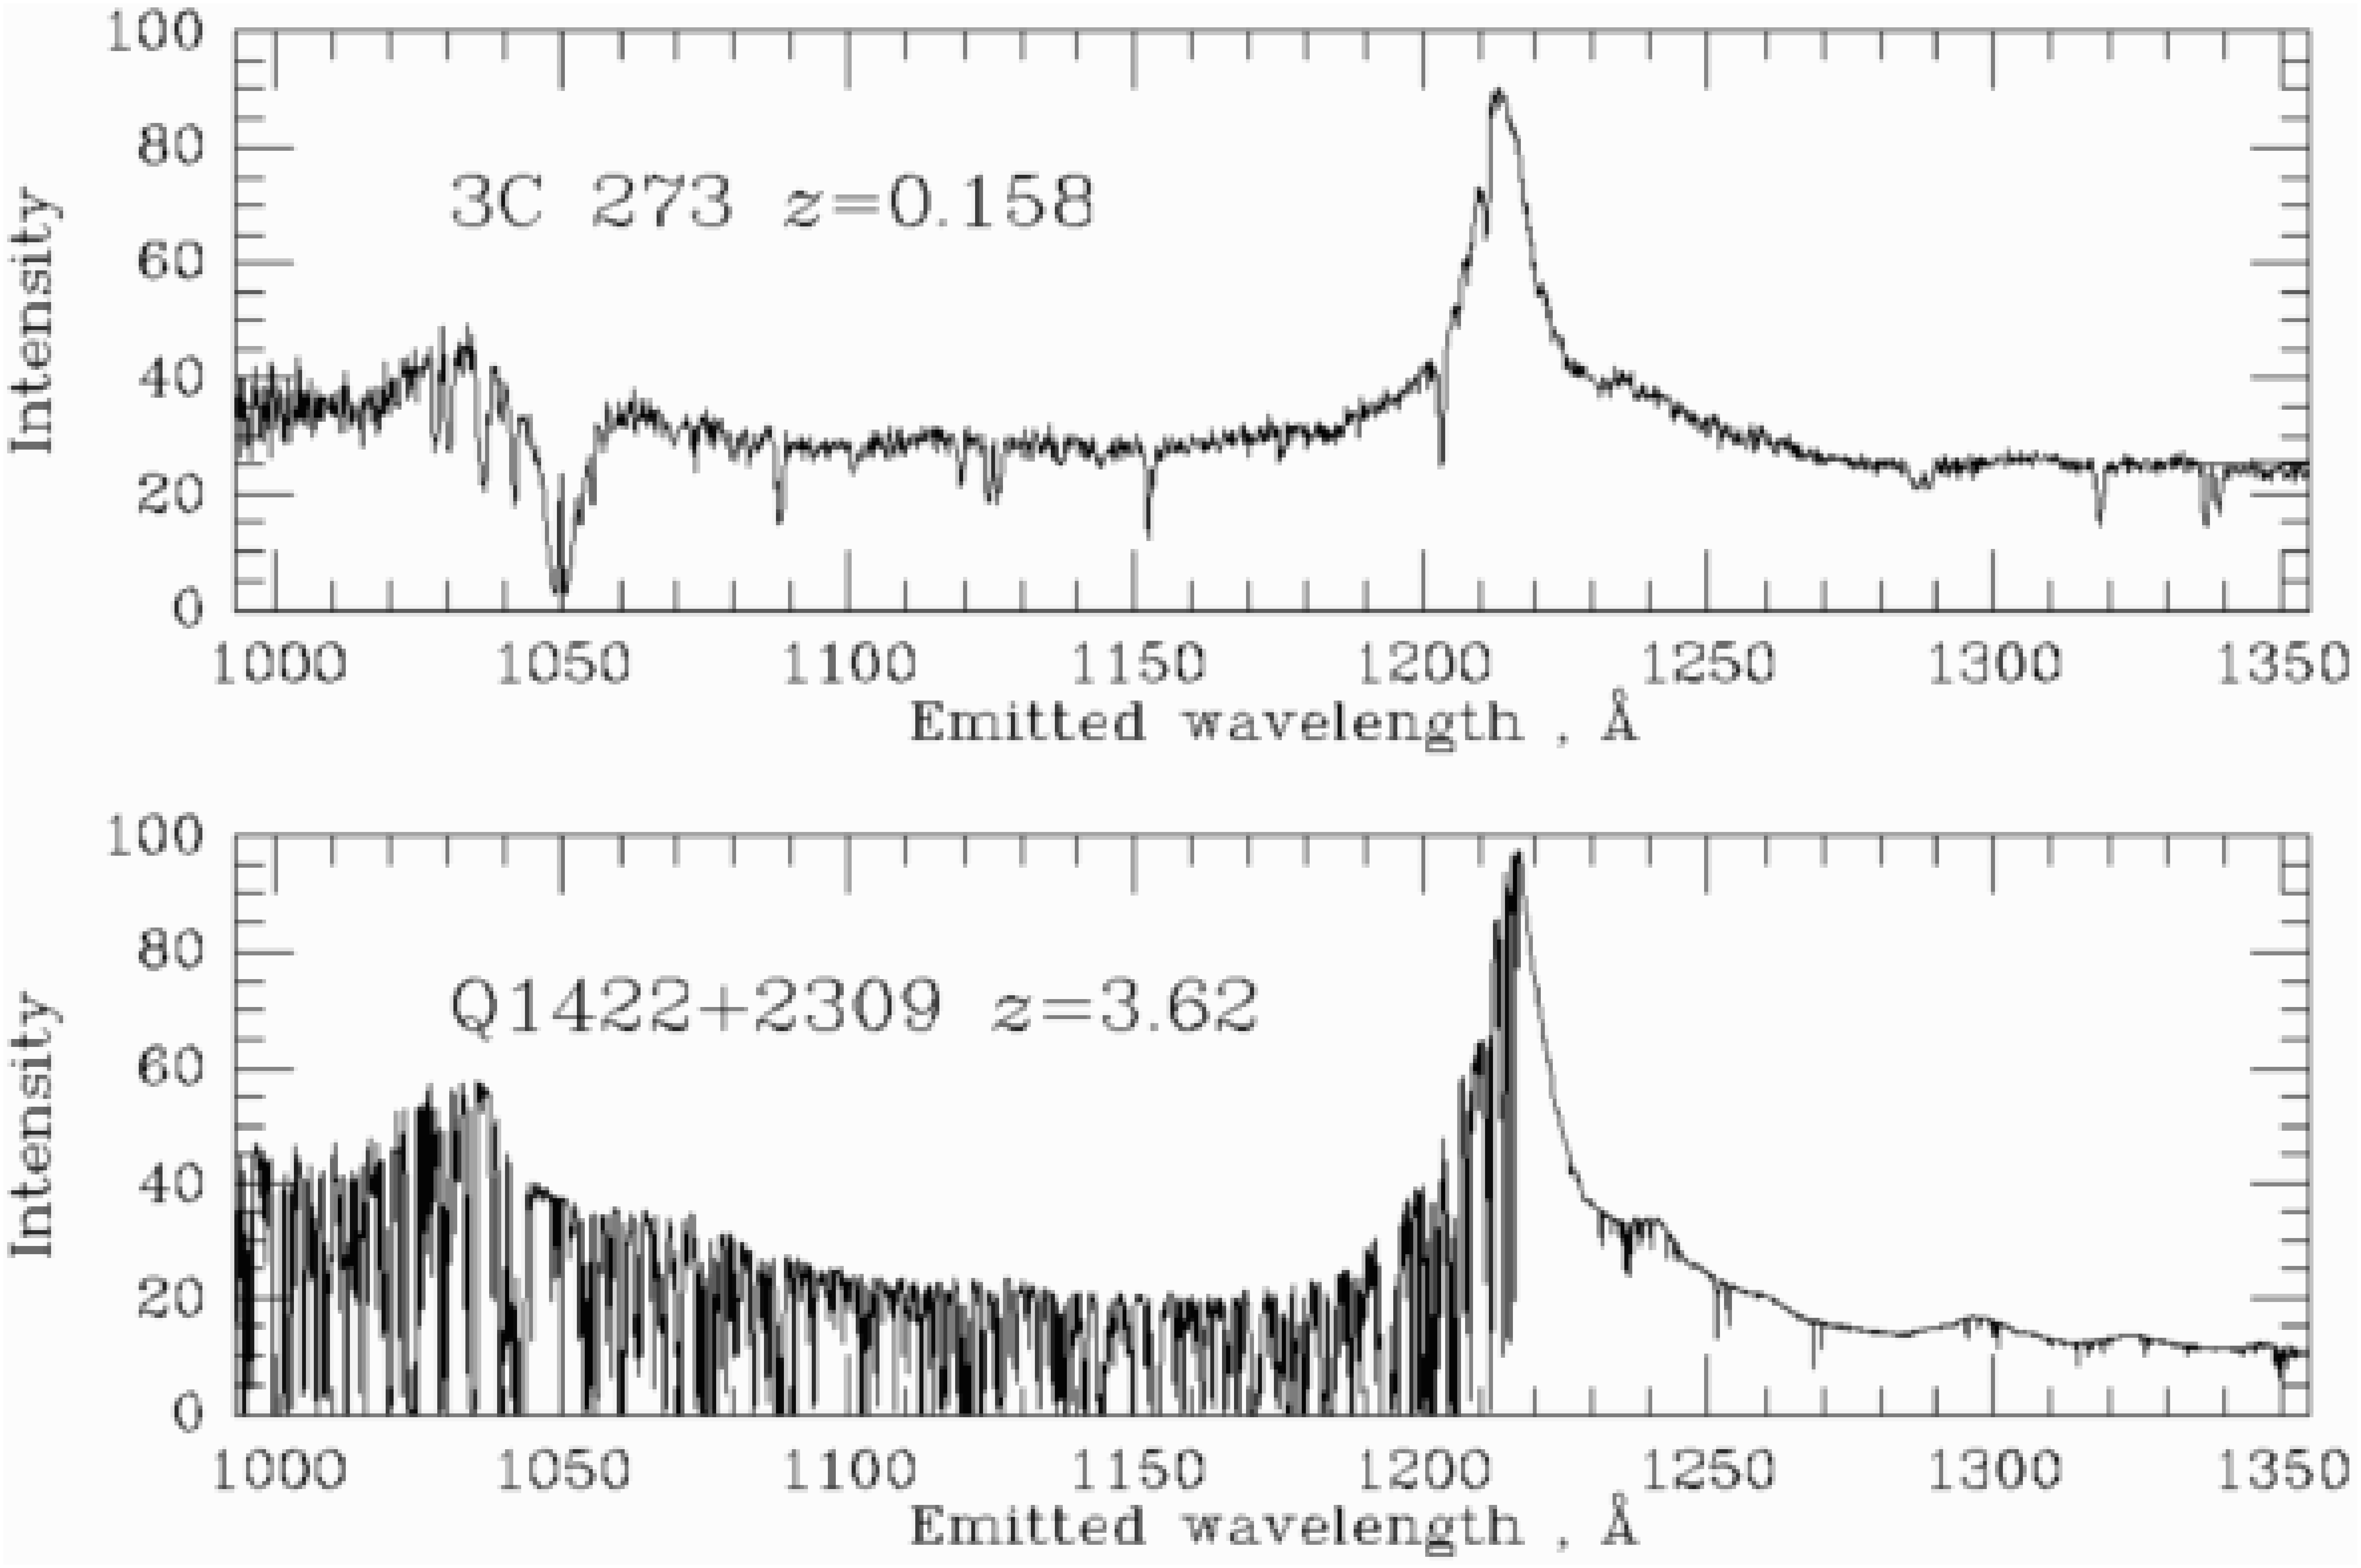
\includegraphics[width=12cm]{Lya-forest-60.eps}
  \caption{Flux as a function of rest-frame wavelength for a quasar at $z = 0.158$ (top) and $z = 3.62$ (bottom). The denser IGM at higher $z$ results in a dense ``forest" of absorption lines blueward of the rest-frame \lya\ line in the lower panel. (Image from {\tt http://www.astro.ucla.edu/})}
  \label{fig:LyaExample}
\end{figure}

At this point, the \lya\ forest should sound like a perfect tool: if we want to map the distribution of neutral hydrogen along the line of sight to a distant bright source, we can simply map each absorption line in the \lya\ forest to a parcel of neutral hydrogen. However, the story becomes complicated here due to the extremely large cross section for \lya\ absorption. Namely, the optical depth\nomenclature[Zp]{Optical Depth}{Optical depth, denoted by $\tau$, is a quantity that describes that likelihood for a photon to be absorbed, usually by a gas. The fraction of photons that will pass through the gas unabsorbed is $e^{-\tau}$.} for \lya\ absorption of a neutral hydrogen gas parcel is approximately

\begin{align}
\tau_{\alpha} &\approx 3.3 \times 10^{4} \xhi (1 + \delta) \left[\dfrac{1+z}{6.5}\right]^{3/2}. \label{eq:tauGP}
\end{align}

Using this expression, we can calculate the minimum neutral fraction needed for a gas parcel at mean density to allow 1\% transmission at $z = 5.5$:

\begin{align}
.01 &= e^{-\tau_{\text{min}}} \implies \tau_{\text{min}} \approx 4.6\\
4.6 &\approx \tau_{\alpha} x_{\text{HI,min}} \\
\implies x_{\text{HI,min}} &\approx 0.00014.
\end{align}


This reveals the fly in the ointment here: even a gas parcel that is 99.9\% ionized will allow less than 1\% transmission at the redshifts of interest for reionization. This allows absorption features to be caused by highly-ionized gas that happens to be over-dense. Therefore, we can not simply map absorption lines in the \lya\ forest to regions of significantly-neutral hydrogen. In fact, the second example quasar we see in Figure \ref{fig:LyaExample} shows significant \lya\ absorption and is located at $z = 3.62$, \textit{much later than the end of reionization}. At this point, the reader may ask what utility does the \lya\ forest have at all? Well, an enormous amount. To name a very few applications outside of reionization, since \lya\ absorption can be caused by matter overdensities, the \lya\ forest can be used to measure the matter power spectrum in the IGM. This, in turn, can be used to measure the baryon acoustic oscillations (BAO), provide lower limits on the mass of the dark matter (\citealt{Viel:2013fqw}), and constrain dark energy, for example. Additionally, absorption features due to damped \lya\ absorbers (DLAs) can be used to measure the primordial deuterium abundance as a test of big bang nucleosynthesis.\\
\textcolor{white}{suspense!}\\
\noindent But how to constrain the EoR?


\clearpage
\subsubsection{Evolution of $\tau_{\text{eff}}$}

% The Gunn-Peterson optical depth to \lya\ photons is \tau_{\text{GP}} = \dfrac{\pi e^2}{m_e c} f_{\alpha} \lambda_{\alpha} H^{-1}(z)n_{\text{HI}}

% Absorption is understood as being caused by the fluctuating Gunn-Peterson effect, low density regions in approximate thermal equilibrium between photoionization heating by the UV background and adiabatic cooling due to the Hubble expansion, rather than discrete \lya\ absorbers.

% By studying the evolution of the average transmitted flux or effective optical depth, one can trace the evolution in the 

% You probably want to re-read and refer to Lidz et al. that discuss that the evolution in the effective optical depth can be replicated by density fluctuations

Perhaps the most common analysis performed on high-redshift quasar spectra in the context of constraining the EoR is measurements of the effective Gunn-Peterson optical depth, defined as

\begin{align}
\langle F \rangle &\equiv e^{-\tau_{\text{eff}}}
\end{align}
\gloss{$\tau_{\text{eff}}$}{The effective Gunn-Peterson optical depth, which is the negative log of the mean transmission over a given redshift bin. Measurements of $\tau_{\text{eff}}$ are often converted into constraints on the photoionizaiton rate}where $\langle F \rangle$ is the averaged transmission fraction over a redshift bin in a quasar/GRB spectrum. Under the assumption of a uniform ionizing background and ionization equilibrium, where the rate that neutral hydrogen atoms are ionized is equal to the rate that ionized hydrogen atoms recombine, the effective optical depth encodes important information about the state of the IGM. In order to see this, we can take a few steps to express the optical depth in terms of the properties of the IGM.\footnote{The following discussion will borrow heavily from \cite{FaucherGiguere:2007jc} and \cite{fan2002evolution}.} First, the Gunn-Peterson optical depth can be expressed as

\begin{align}
\tau_{\text{GP}} &= \dfrac{\pi e^{2}}{m_{e} c} f_{\alpha}\lambda_{\alpha} \dfrac{n_{\text{HI}}}{H(z)}, \label{eq:tauGP}
\end{align}

where $H(z)$ is the Hubble parameter at redshift $z$, $e$ is the charge of the electron, $m_e$ is the electron mass, $c$ is the speed of light, $\lambda_{\alpha}$ is the \lya\ wavelength, $f_{\alpha}$ is the quantum mechanical oscillator strength, and $n_{\text{HI}}$ is the number density of neutral hydrogen atoms\gloss{HI}{Neutral hydrogen}\gloss{HII}{Ionized hydrogen}\gloss{HeI}{Neutral helium}\gloss{HeII}{Singly-ionized Helium}\gloss{HeIII}{Fully-ionized helium}\gloss{$f_{\alpha}$}{Quantum mechanical oscillator strength for the \lya\ transition}\gloss{$e$}{Charge of the electron}\gloss{$\lambda_{\alpha}$}{Wavelength of the \lya\ transition}\gloss{$m_e$}{Mass of the electron}. All of these quantities are known with the exception of the number density of neutral hydrogen atoms. To find this, we first utilize the statement of ionization equilibrium:

\begin{align}
\Gamma_{\text{HI}} n_{\text{HI}} &= R(T)n_{e}n_{\text{HII}} \label{eq:IonEquilibrium} \\
n_{\text{HI}} &= \dfrac{R(T) n_{e} n_{\text{HII}}}{\Gamma_{\text{HI}}} \label{eq:nH}\\
x_{\text{HI}} &= \dfrac{R(T)n_e}{\Gamma_{\text{HI}}} \label{eq:xHI}
\end{align}

where $\Gamma_{\text{HI}}$\gloss{$\Gamma_{\text{HI}}$}{Photoionization rate for hydrogen atoms. This depends on the number,  location, and properties of the ionizing sources.} is the photoionization rate due to the ionizing sources, $n_{e}$ is the number density of free electrons, $n_{\text{HII}}$ is the number density of ionized hydrogen atoms (protons), and $x_{\text{HI}}$ is the hydrogen neutral fraction. The left-hand side of Eq. \ref{eq:IonEquilibrium} represents the rate of photoionizations per volume and the right hand side represents the rate of hydrogen recombinations per volume. Under the assumption of ionization equilibrium with a uniform ionizing background, the presence of any transmission suggests $n_{\text{HII}} \approx n_{\text{HI}} + n_{\text{HII}} = n_{\text{H}}$ and 

\begin{align}
\bar{n}_{\text{H}} &= \frac{\rho_{c}(z)\Omega_{b}(z)X_{\text{H}}}{m_p} = \dfrac{3H^{2}(z)}{8\pi G} \dfrac{\Omega_{b}(z) X_{\text{H}}}{m_{p}} \\
&= \dfrac{3H_{0}^{2}\Omega_{b,0}}{8\pi G} \dfrac{X_{\text{H}}}{m_p}(1+z)^{3}\\
n_{\text{H}} &= (1+\delta) \bar{n}_{\text{H}}. \label{eq:ntot}
\end{align}

In this expression, $\rho_c$\gloss{$\rho_{c}$}{Critical energy density for a flat Universe} is the critical density for a flat Universe, $\Omega_{b}$\gloss{$\Omega_b$}{Baryon density in units of the critical density} is the baryon density in units of the critical density, $X_{\text{H}}$\gloss{$X_{\text{H}}$}{The fraction of baryonic mass in the form of hydrogen} is the fraction of baryonic mass in the form of hydrogen, $m_{p}$ is the mass of the proton which is effectively equal to the mass of the hydrogen atom, and $\delta \equiv (\rho-\bar{\rho})/\bar{\rho}$\gloss{$\delta$}{The local mass overdensity in units of the cosmic mean} is the local mass overdensity in units of the cosmic mean. A subscript of ``0" denotes that these are present-day values and $\bar{n}_{\text{H}}$ denotes the average of $n_{\text{H}}$. Thus, as we expect, this expression is essentially equal to the mass density of hydrogen atoms in the Universe divided by the mass per atom.\footnote{It may be interesting to note that this value corresponds to 0.2 hydrogen atoms per cubic meter today and roughly $\sim$50 hydrogen atoms per cubic meter at $z = 5.5$. It is very empty out there.}  The expression for the electron number density should be the same, since each ionized hydrogen atom releases one free electron. However, it is probably the case that helium is singly ionized along with hydrogen, so the number density will increase according to:

\begin{align}
\bar{n}_e &= \bar{n}_{\text{H}} + \bar{n}_{\text{He}} = \dfrac{3H^2}{8\pi G}\left( \dfrac{X_{\text{H}}}{m_{p}} + \dfrac{(1 - X_{\text{H}})}{4m_{p}} \right) \\
&\approx 1.08 \bar{n}_{\text{H}}. 
\end{align}

However, for simplicity here, let us approximate $n_{\text{tot}} \equiv n_{e} \approx n_{\text{H}}$. The quantity $R(T)$ in Eq. \ref{eq:IonEquilibrium} is the recombination rate, which is equal to (\citealt{Hui1997}):

\begin{align}
R(T) &\approx 4.2 \times 10^{-13}\left( \dfrac{T}{10^{4} K}\right)^{-0.7} \text{cm}^{3}\sec^{-1}. \label{eq:RecombinationRate}
\end{align}

For $\delta \lesssim 5$, \cite{Hui1997} showed that the temperature and density follow the relationship

\begin{align}
T &\approx T_{0}(1+\delta)^{\gamma - 1} \label{eq:Trelation}
\end{align}

where $T_0$ is the temperature of a parcel of gas at mean density, and $\gamma$ is the slope of the temperature-density relation. For compactness, let's define $R_{4} \equiv R(T=10^{4}K)$. At this point, we are ready to combine Eq. \ref{eq:Trelation}, \ref{eq:RecombinationRate}, \ref{eq:ntot}, \ref{eq:nH}, and \ref{eq:tauGP} to get an expression for $\tau_{\text{GP}}$:

\begin{align}
\tau_{\text{GP}} &= \dfrac{\pi e^2}{m_e c}\dfrac{f_{\alpha}\lambda_{\alpha}}{H(z)} \dfrac{R_{4}(1+\delta)^{-0.7(\gamma - 1)}\bar{n}_{\text{tot}}^{2}(z)(1+\delta)^2}{\Gamma_{\text{HI}}}\\
&= \dfrac{\pi e^2}{m_e c}\dfrac{f_{\alpha}\lambda_{\alpha}}{H(z)} \dfrac{R_4 \bar{n}_{\text{tot}}^{2}(z)}{\Gamma_{\text{HI}}} (1+\delta)^{2-0.7(\gamma-1)}. \label{eq:tauGPfinal}
\end{align}

Finally, we have an expression for the \lya\ optical depth in terms of several properties of the IGM. The primary unknown in the above expression is the photoionization rate, which is a very complicated parameter which depends on the number, intensity, spectrum, and proximity of ionizing sources among other things. A common assumption in these types of analyses is that the photoionization rate is approximately spatially uniform. This seems like a plausible assumption in a post-reionization Universe, when the mean free path of ionizing radiation is long allowing any given gas parcel can receive ionizing radiation from many sources. On the other hand, early in reionization, the Universe is opaque to ionizing radiation and gas parcels tend to only see sources within their own ionized regions. Regardless, with this approximation, the observed mean transmission in a region of the spectrum is akin to an average of Eq. \ref{eq:tauGPfinal} marginalizing over the density field:

\begin{align}
\left\langle F \right\rangle &= \int \dd \delta\ e^{-\tau(\delta)} P(\delta) \equiv e^{-\tau_{\text{eff}}}.
\end{align}


 As such, an intriguing question is, if you have a model for the probability distribution of the underlying density field, what (uniform) value of $\Gamma_{\text{HI}}$ will yield a value for $\left\langle F \right\rangle$ that is consistent with observations? This question has received a lot of attention ({\bf cites}) and has led to many measurements of the photoionization rate. With estimates of the photoionization rate in hand, we can utilize Eq. \ref{eq:xHI} in order to obtain measurements of the IGM neutral fraction in each redshift bin in the spectra in order to gauge the progress of the EoR. Results for measurements of $\Gamma_{\text{HI}}$ and $\axhi$ via this method, performed by \cite{Fan2006a}, are shown in Figure \ref{fig:tauEffResults}. This figure demonstrates that, using $\tau_{\text{eff}}$ and the assumption of ionization equilibrium, estimates of the neutral fraction are exceedingly small for $z \lesssim 6$. This argument has played a large part in forming the common knowledge that reionization has ended by $z = 6$. 

\begin{figure}[!p]
  \centering
  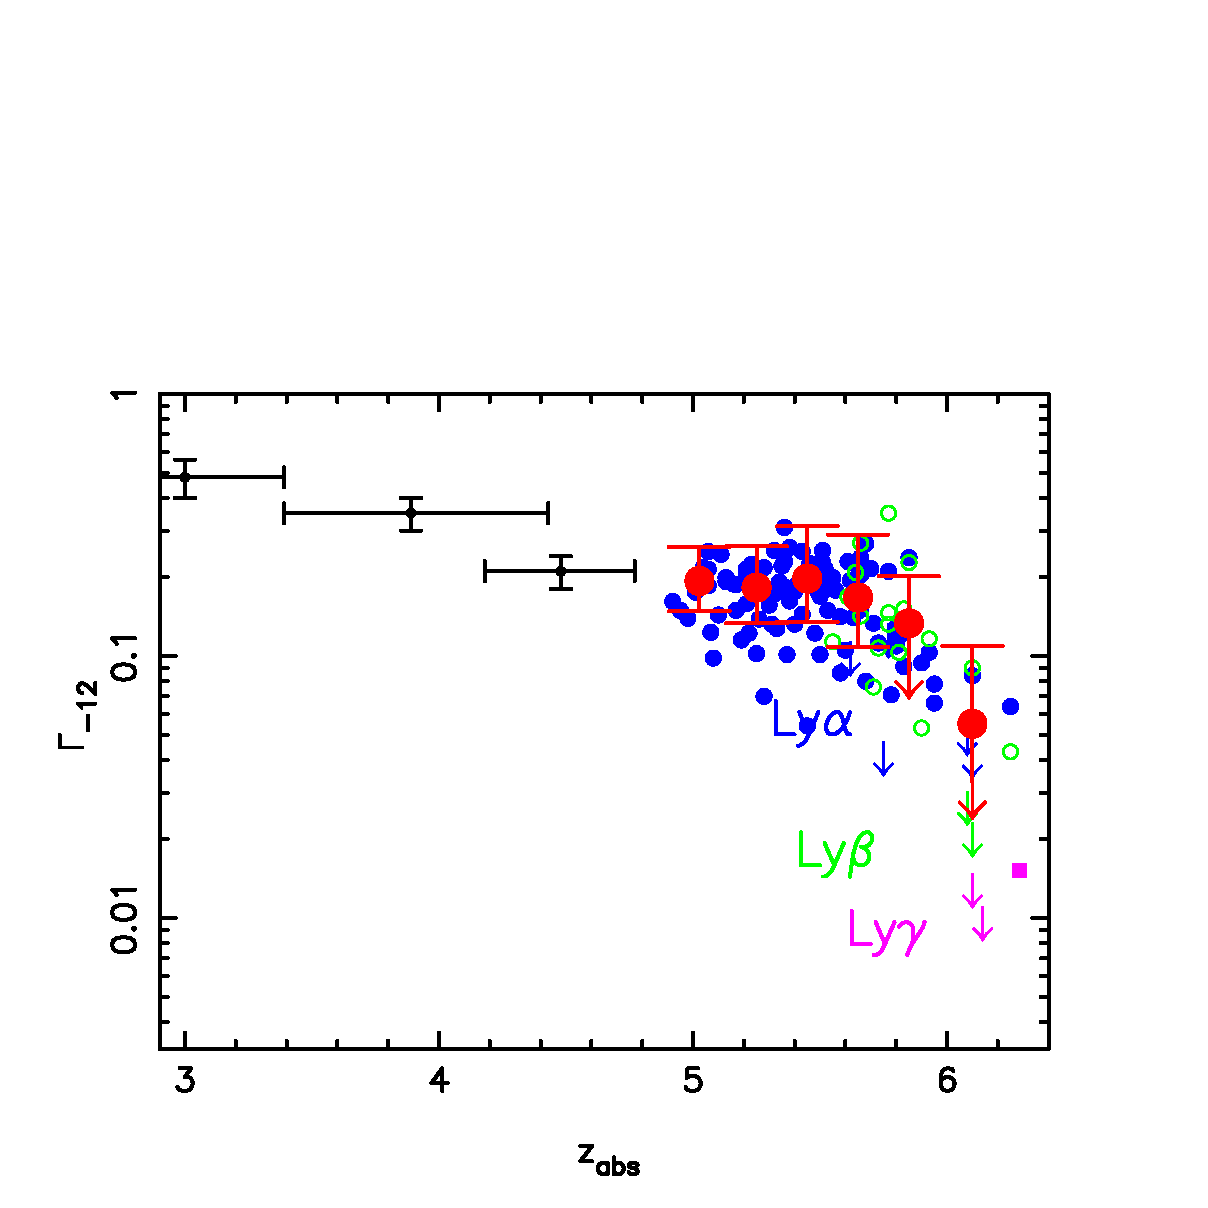
\includegraphics[width=8cm]{Fan.gamma.eps}
  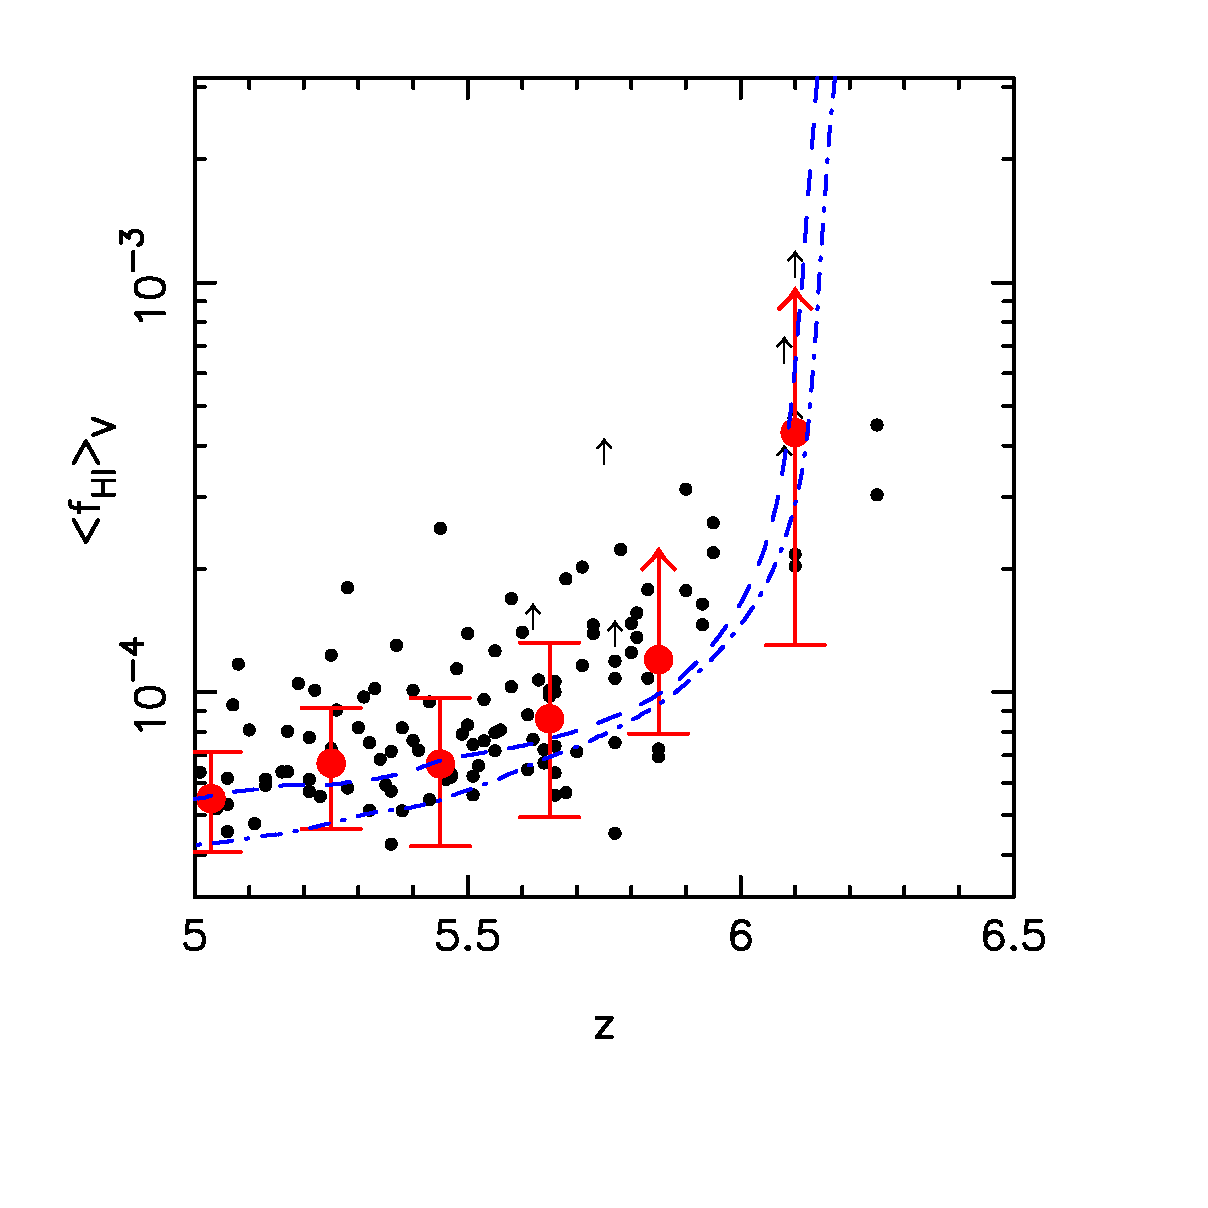
\includegraphics[width=8cm]{Fan.fHv.eps}
  \caption{Measurements of $\Gamma_{\text{HI}}$ (top) and $\axhi$ from \cite{Fan2006a} (bottom).}
  \label{fig:tauEffResults}
\end{figure}


Despite the widespread analysis of $\tau_{\text{eff}}$ in constraining the end of reionization, the interpretation of $\tau_{\text{eff}}$ is quite complicated.\footnote{For a more thorough discussion of controversial aspects of these constraints, see the intro for \cite{McGreer:2011dm}.} First, accepting the assumption of the IGM being in ionization equilibrium with a uniform $\Gamma_{\text{HI}}$ is tantamount to assuming that reionization has ended. Specifically, as discussed in \S \ref{sec:CosmicContext}, reionization is likely a highly inhomogeneous process with ionized bubbles forming around the brightest sources, growing, and eventually overlapping. During the period prior to complete overlap, regions of neutral hydrogen will be shielded from the ionizing radiation while ionized bubbles will experience a very large $\Gamma_{\text{HI}}$. This is not reflected in Eq. \ref{eq:IonEquilibrium} and so we expect conclusions derived from this method to be unreliable when we begin to push up against the end of reionization. Additionally, interpretation of the level of flux in quasar spectra in the context of reionization is further complicated by the fact that quasars likely reside in very atypical parts of the Universe. Specifically, \cite{Lidz:2007mz} show that it is likely that some quasar lines of sight will pass through mostly ionized gas even up to neutral fractions of $\axhi \sim 0.5$. 

%\subsubsection{Dark Gap Sizes}
%
%Yeah, so the main point we want to (briefly) drive home here is that previous constraints on $\axhi$ from the use of dark gap statistics probably assumed a uniform $\Gamma_{\text{HI}}$, which is equivalent to assuming reionization has already ended anyway. 
%
%Fan says imperfect sky subtraction in regions with strong OH lines can cause significant residuals resulting in an \textit{underestimate} in the dark gap size. Although, it seems like they don't allow any room for noise fluctuations in what they constitute a dark gap???

\clearpage
\subsubsection{Dark Pixel Covering Fraction}

As demonstrated in the previous section, interpreting measurements of the effective optical depth in the context of reionization is complicated and can rely on controversial assumptions. However, an alternative approach is to consider what constraints can be made without resorting to such assumptions. In this regard, an important method in estimating $\axhi$ from high-redshift quasar observations is the dark pixel covering fraction. This approach is rooted in the fact that neutral parcels of gas are certain to result in saturated absorption in quasar spectra due to their optical depths being $\tau_{\text{HI}} \gtrsim 10^4$ (Eq. \ref{eq:tauGP}). Therefore, a reliable upper bound on the neutral fraction at a given redshift can be estimated by the fraction of pixels in quasar spectra that are completely absorbed at that redshift. 

An obvious drawback of this method is that, at $z \sim 6$, overdense yet ionized regions will also result in saturated absorption and will significantly increase this upper bound on the neutral fraction. One approach to combat this effect is to incorporate the \lyb\ forest into the analysis. The optical depth for Lyman-series transitions scales as $f\lambda$, where $f$ is the oscillator strength of the transition and $\lambda$ is the corresponding wavelength. Therefore, the analogous expression of Eq. \ref{eq:tauGP} for \lyb\ is:

%Useful quantities:                                                                                                   
% Oscillator Strengths                                                                                                
% f_21 = 0.4162 (1s-2p)  lambda_21 = 1215.67 AA                                                                       
% f_31 = 0.0791 (1s-3p)  lambda_31 = 1025.72 AA                                                                       
% f_32 = 0.4349 (2s-3p)  lambda_32 = 6562.74 AA 
\begin{align}
\tau_{\beta} &= \tau_{\alpha} \times \dfrac{f_{\beta}\lambda_{\beta}}{f_{\alpha}\lambda_{\alpha}} \approx 5.3 \times 10^{3} \xhi (1 + \delta) \left[\dfrac{1+z}{6.5}\right]^{3/2}. \label{eq:tauGPB}
\end{align}

where $f_{\alpha} = 0.4162$, $\lambda_{\alpha} = 1216 \AA$, $f_{\beta} = 0.0791$, and $\lambda_{\beta} = 1026\AA$. From this expression, we can see that a mean-density parcel of neutral gas should cause saturated absorption in both the \lya\ and \lyb\ transitions. Meanwhile, ionized overdense regions are less likely to cause saturated absorption as their optical depth in \lyb\ is reduced by a factor of $f_{\beta}\lambda_{\beta}/f_{\alpha}\lambda_{\alpha} \approx 1/6$. Therefore, limits from the dark-pixel covering fraction may be improved by requiring simultaneous absorption in both \lya\ and \lyb\ as part of the definition of a dark pixel. Additionally, the \lyb\ dark pixel covering fraction on its own is a viable tool for establishing an upper bound on the neutral fraction, although foreground \lya\ absorption may undo some of the gains from the lower $\tau_{\beta}$ value. In practice, all three approaches (requiring \lya, \lyb, and \lya +\lyb\ absorption) are used. 

This procedure faces several complications when actually carried out, however. First, quasar observations are subject to the noise from the night sky which effectively adds mean-zero random noise to the spectra. The addition of this random noise can result in spurious transmission in pixels that otherwise would have been completely absorbed. Therefore, to measure the dark pixel fraction in quasar spectra, one first needs to create a suitable definition of what qualifies as a ``dark" pixel. One approach here is to define dark pixels as having transmission below some threshold defined in terms of the noise standard deviation, $\sigma_{\text{N}}$. This presents us with a tradeoff, however, since larger thresholds will reduce the number of neutral pixels we miss but also increase the number of ionized pixels that get incorporated into the dark pixel population. Alternatively, if we are presented with median-zero noise, then half of all truly-absorbed pixels will result in negative flux values, on average. This presents the possibility of using twice the negative-flux-pixel covering fraction as an estimate of the dark-pixel covering fraction (or four times, in the case of requiring \lya +\lyb\ absorption) (\citealt{McGreer:2014qwa}). 

A second complication is that, since pixels have a finite width, their transmission values effectively represent an average of the transmission over some region in the spectra. If the pixel width is large enough, then it is possible for a pixel to have non-zero transmission despite corresponding to a physical region that contains significantly-neutral gas. For example, if the physical region in space associated with the pixel is 80\% composed of completely-neutral gas and 20\% composed of completely ionized gas which allows full transmission, then the transmission of that pixel will be 20\% and will likely not qualify as a ``dark pixel" despite containing neutral gas. Thus, even in a measurement as seemingly-simple as the dark-pixel covering fraction, these details must be kept in mind when interpreting results. 

Regardless, \cite{McGreer:2011dm} and \cite{McGreer:2014qwa} apply the dark-pixel covering fraction approach to 22 high-redshift quasar spectra to produce the constraints on $\axhi$ shown in Figure \ref{fig:McGreer}. Dimly-colored points correspond to \cite{McGreer:2011dm} while bold-colored points correspond to \cite{McGreer:2014qwa}. These results present a very different interpretation than using $\tau_{\text{eff}}$ measurements while using the same data. Namely, that model-independent constraints have a hard time conclusively confirming the common knowledge that reionization has ended by $z \sim 6$.\footnote{The authors here do go on to focus on a high-resolution subset of their quasar observations presented in \cite{McGreer:2014qwa} in order to argue in favor of an end to the EoR by $z \sim 6$. However, the precise interpretation of the spectra is complex, as discussed herein.} 

\begin{figure}[!p]
  \centering
  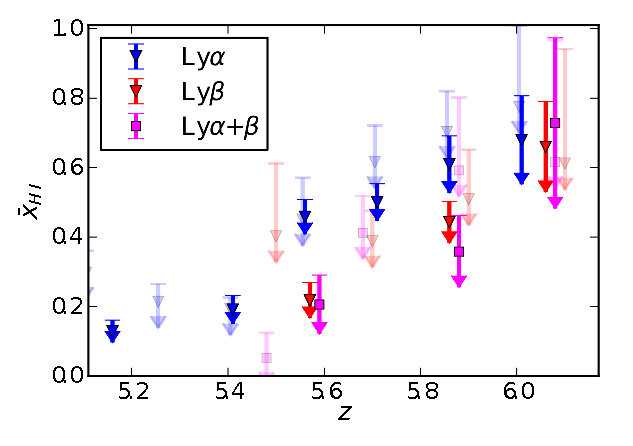
\includegraphics[width=8cm]{xhi_newdata.eps}
  \caption{Current limits on $\axhi$ derived from the dark-pixel covering fraction in \cite{McGreer:2014qwa}. Lightly-shaded points are older limits obtained in \cite{McGreer:2011dm}.}
  \label{fig:McGreer}
\end{figure}


\clearpage
\subsubsection{Damping Wing Redward of \lya}\label{sec:IntroDampingWing}

Much of the difficulties in using the \lya\ forest to constrain the timing of the EoR can be boiled down to the following problem: interpreting \lya\ absorption in high-redshift quasar spectra is difficult because both neutral and ionized gas can result in saturated absorption. Therefore, it is worth asking if there are any ways to break this degeneracy in \lya\ absorption in order to determine which absorption is likely due to neutral hydrogen. One potential approach toward this goal, which has received much attention (\citealt{Chornock:2013una}, \citealt{Chornock:2014fva}, \citealt{Mortlock2011}, \citealt{Bolton:2011vb}), is looking for the hydrogen damping wing redward of the \lya\ line. 


To understand this approach, let us first understand what the hydrogen damping wing is. For many applications, it is suitable to consider an atom's ability to absorb radiation as a series of delta functions in frequency: when incident radiation has a frequency exactly coinciding with the energy of the transition, then there is a non-zero probability for absorption and zero probability otherwise. In reality, the probability of absorbing a photon of a given frequency, e.g., the line profile, is a continuous distribution which, while small for frequencies $\nu \neq \nu_{0}$, is non-zero. 


The intrinsic line profile for the \lya\ transition in the hydrogen atom can be seen as arising from the time/energy uncertainty principle, $\Delta E \cdot \Delta t \gtrsim \hbar$. Specifically, the finite lifetime of the $n = 2$ excited state implies the existence of a range of energies that can excite, or result from, the transition. The distribution of this range of energies follows a Lorentzian distribution\gloss{Lorentzian Distribution}{Probability distribution for the ratio of two standard-normal-distributed variables. This distribution also describes the intrinsic line profile for absorption lines.}:\footnote{A quantum-mechanical discussion of this result can be found in \S 5.8 of \cite{sakurai2011modern}. A classical derivation can be found in \S 3.6 of \cite{rybicki1979radiative}.}

\begin{align}
\phi(\nu) &= \frac{1}{\pi} \dfrac{\Gamma/4\pi^{2}}{(\nu - \nu_{0})^{2} + (\Gamma/4\pi)^2}
\end{align}

with the corresponding absorption cross section

\begin{align}
\sigma_{\alpha}(\nu) &= \dfrac{\pi e^2}{m_{e}c} f_{\alpha} \phi(\nu). \label{eq:IntroLineProfile}
\end{align}

The ``damping wing" refers to the $\sigma \sim 1/(\nu-\nu_{0})^{2}$ behavior far from line center. This can be used to break the degeneracy between HII absorption and HI absorption because the optical depth is so much smaller in the damping wing that, without significantly-neutral gas (optical depth scales with neutral fraction), the optical depth at such frequency separations will not be sufficient to cause absorption. Furthermore, the damping wing has a distinct shape which can be fit for in order to infer the properties of the neutral gas which sources it. 


While the damping wing from an isolated neutral region in a sea of fully-ionized, $\tau = 0$ hydrogen would stand out like a sore thumb, in reality absorption from the surrounding dense, yet ionized, gas will punctuate the damping wing with additional absorption features and will make it harder to detect. This makes the prospect of looking for isolated damping wings in typical regions in quasar spectra unappealing. However, photons emitted slightly \textit{redward} of \lya\ cannot be absorbed by dense ionized gas since ionized gas has a negligible optical depth for $\nu \neq \nu_{\alpha}$. Neutral hydrogen, on the other hand, \textit{will} allow absorption to take place redward of \lya\ due to the significant optical depth in the damping wing. Because of this, searches for the damping wing slightly redward of the \lya\ line will be able to avoid nuisance absorption from neighboring ionized gas.


We show a famous example of a potential damping-wing detection in Figure \ref{fig:Mortlock}, taken from \cite{Mortlock2011}. This shows a region of the transmission spectrum for a quasar at redshift $z = 7.085$ (ULAS J1120+0641). The fractional transmission nearby the \lya\ line exhibits a gradual recovery from almost complete absorption at $\lambda < \lambda_{\alpha}$ to almost complete transmission at $\lambda > \lambda_{\alpha}$, occurring over a wavelength interval consistent with a hydrogen damping wing. The curves in blue show models for damping wing absorption associated with an IGM with neutral fraction $\axhi = 0.1$ (top), 0.5 (middle), and 1 (bottom) with a sharp ionization front at a distance of 2.2Mpc from the quasar. In green, a model for the absorption profile of a Damped \lya\ Absorber (DLA, see glossary for definition)\gloss{DLA}{Damped \lya\ Absorber. These are dense, isolated clouds of gas with extremely high column densities of neutral hydrogen, $N_{\text{HI}} \gtrsim 2\times10^{20}\cm^{-2}$ sufficient to exhibit damping-wing absorption. These are thought to source galaxy formation and are not part of the diffuse IGM which we want to study for reionization purposes.} with column density $N_{\text{HI}} = 4\times10^{20}\text{cm}^{-2}$ located 2.6 Mpc from the quasar is shown. Thus, the transmission profile appears consistent with both a significantly-neutral ($\axhi > 0.1$) IGM or a proximate DLA. However, \cite{Simcoe} perform a search for metal lines, which typically accompany DLA absorption, and find that the gas is extremely metal-poor. This bolsters the claim that the damping-wing absorption seen in this example is, in fact, due to diffuse neutral hydrogen in the IGM. 


\begin{figure}[!p]
  \centering
  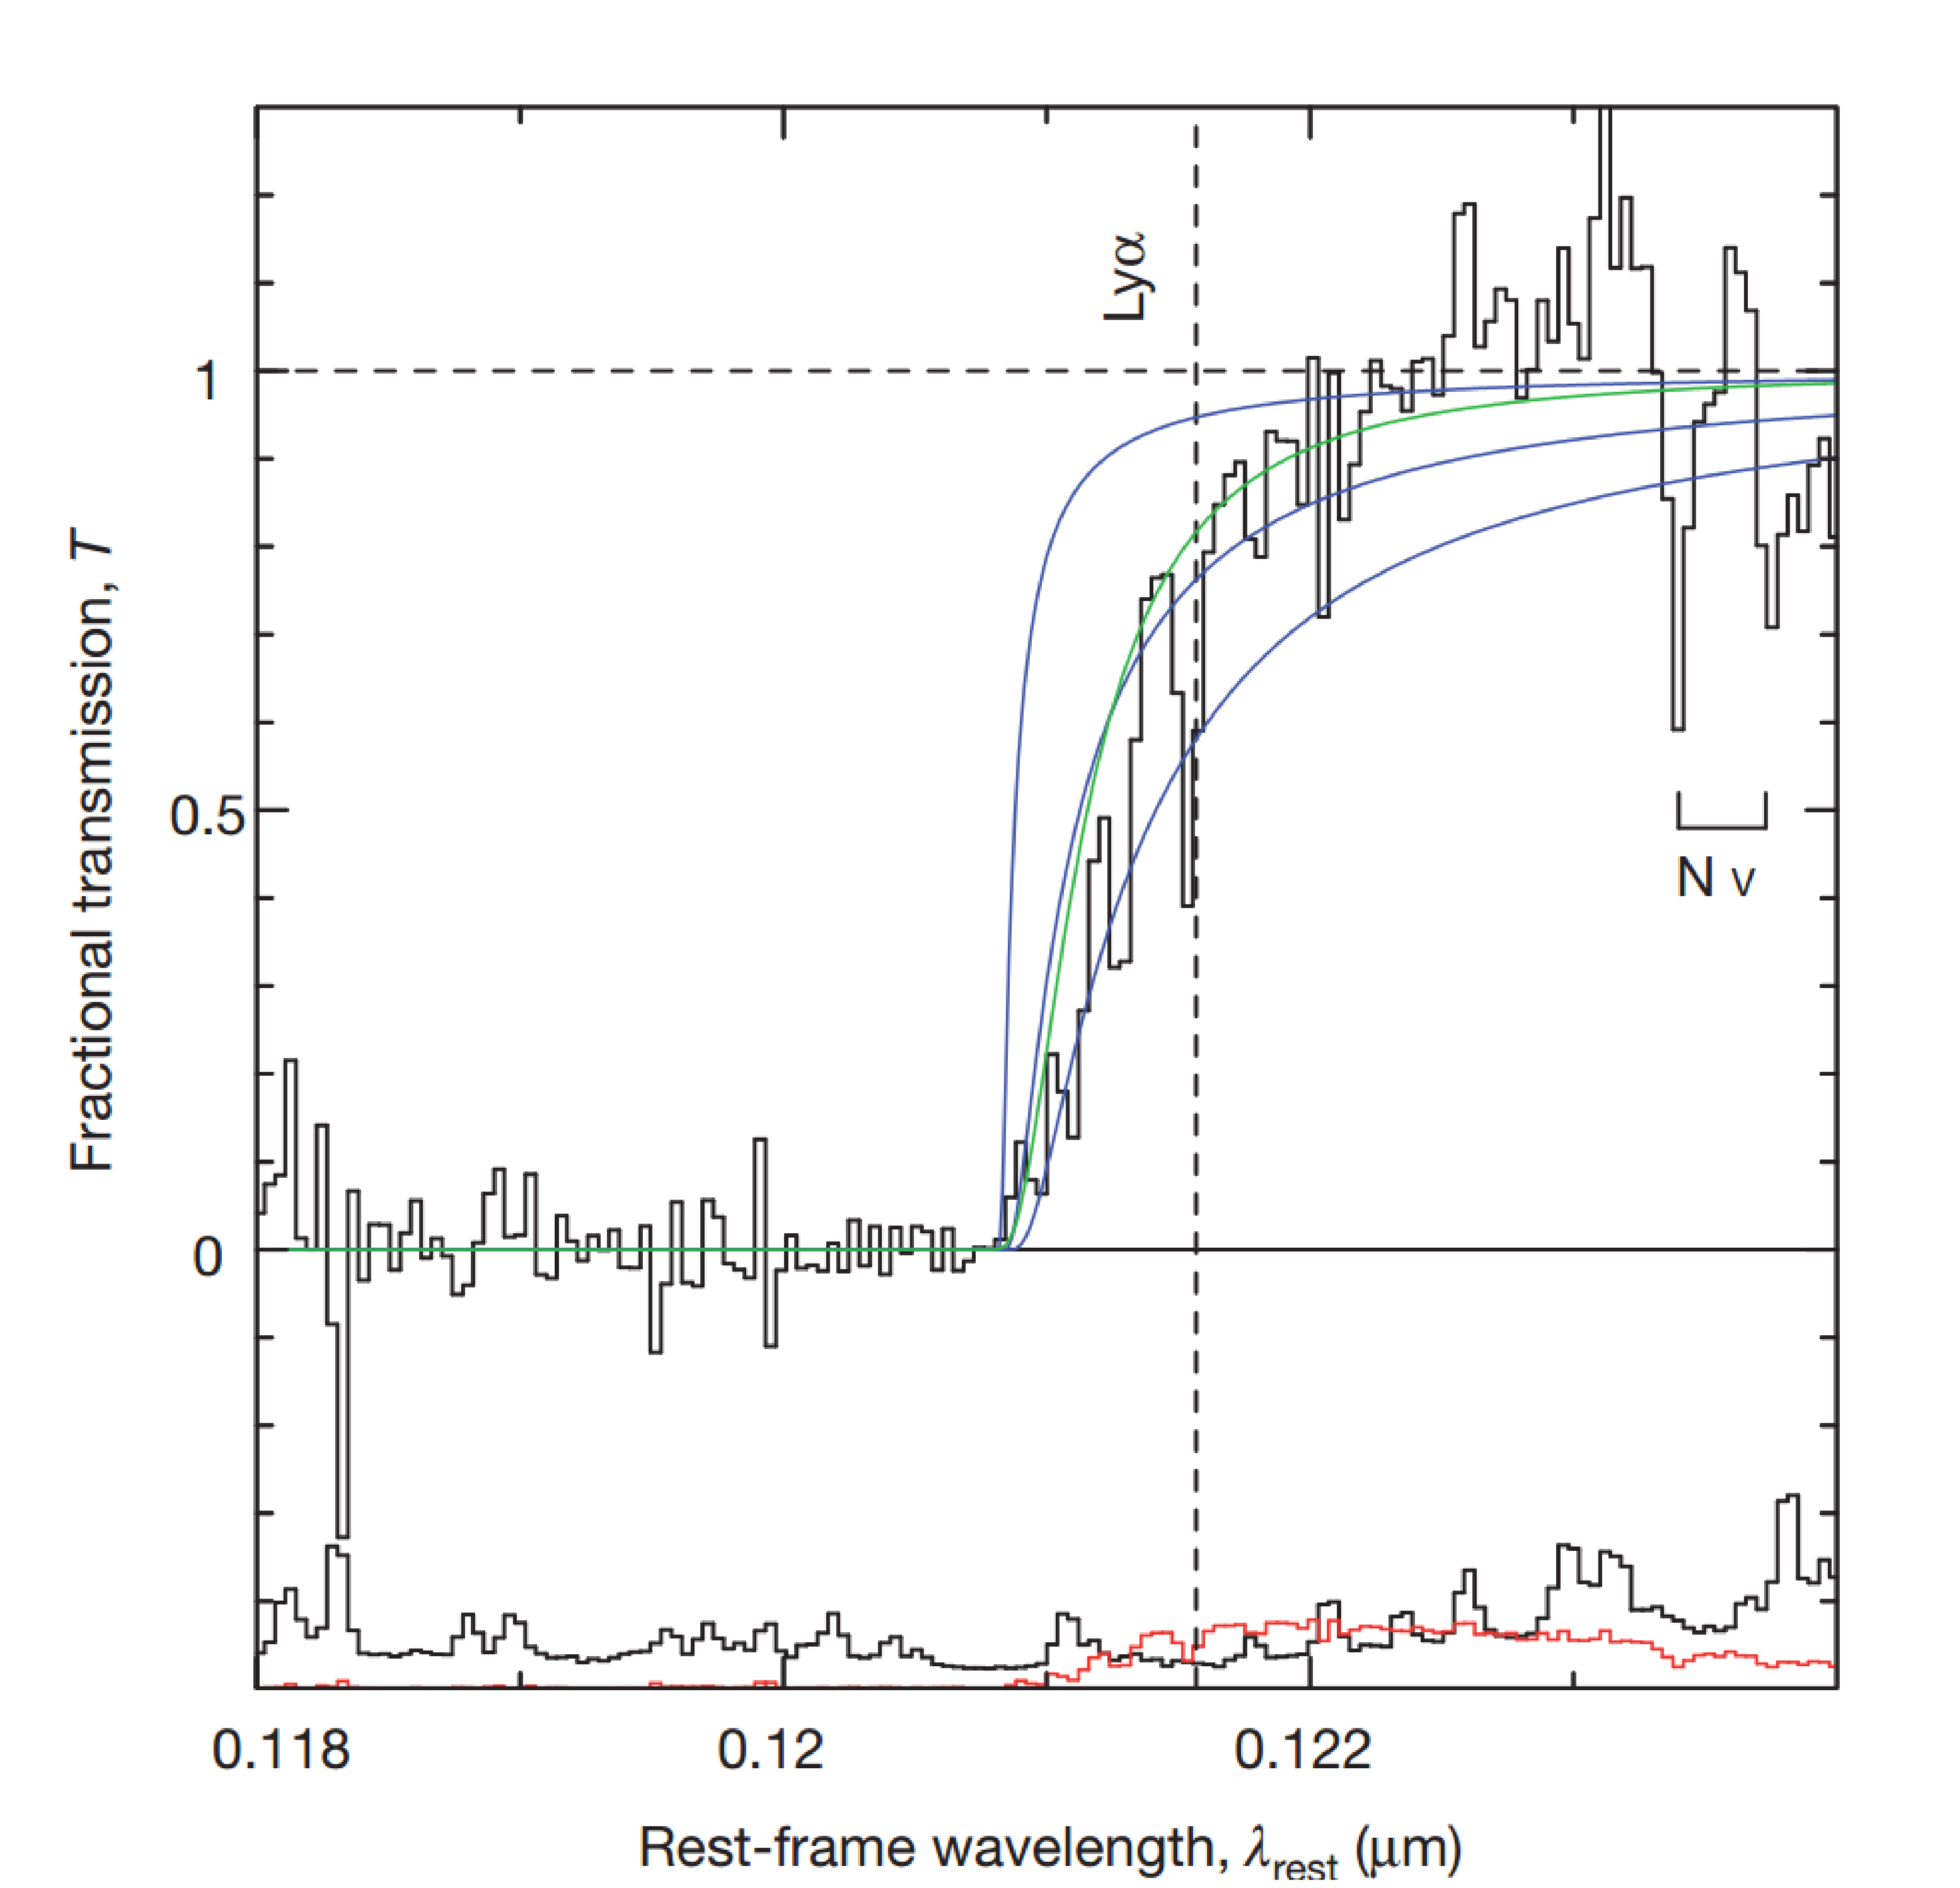
\includegraphics[width=8cm]{z7p085_DampingWing.eps}
  \caption{Quasar ULAS J1120+0641 identified at redshift $z = 7.085$ along with several fits for the damping wing.}
  \label{fig:Mortlock}
\end{figure}


Other searches for damping-wing absorption redward of \lya\ have been carried out on, for example, GRB 130606A (\citealt{Chornock:2013una}) and GRB 140515A (\citealt{Chornock:2014fva}). These authors looked for the damping wing in the spectra of GRB afterglows at redshift $z = 5.913$ and $z = 6.33$, respectively. A non-detection in the spectra of the $z = 5.913$ GRB allowed the authors to place a $2\sigma$ limit on the nearby IGM neutral fraction of $\axhi < 0.11$. Similarly, no strong evidence of a damping wing was found in the spectrum of GRB140515A, shown in Figure \ref{fig:GRB140515A}. The right-hand panel shows the transmission fraction nearby the \lya\ transition, which is equally-well fit by pure host absorption (blue, $N_{\text{HI}} = 10^{18.62}\text{cm}^{-2}$), pure IGM absorption from gas at $6.0 \leq z \leq 6.328$ with $\axhi = 0.056$ (red), and a hybrid model with a host absorber lying within an ionized bubble with $R = 10$ comoving Mpc met by an IGM with $\axhi = 0.12$ (green). As such, they argue against a significantly-neutral IGM at this redshift.  

\begin{figure}[!p]
  \centering
  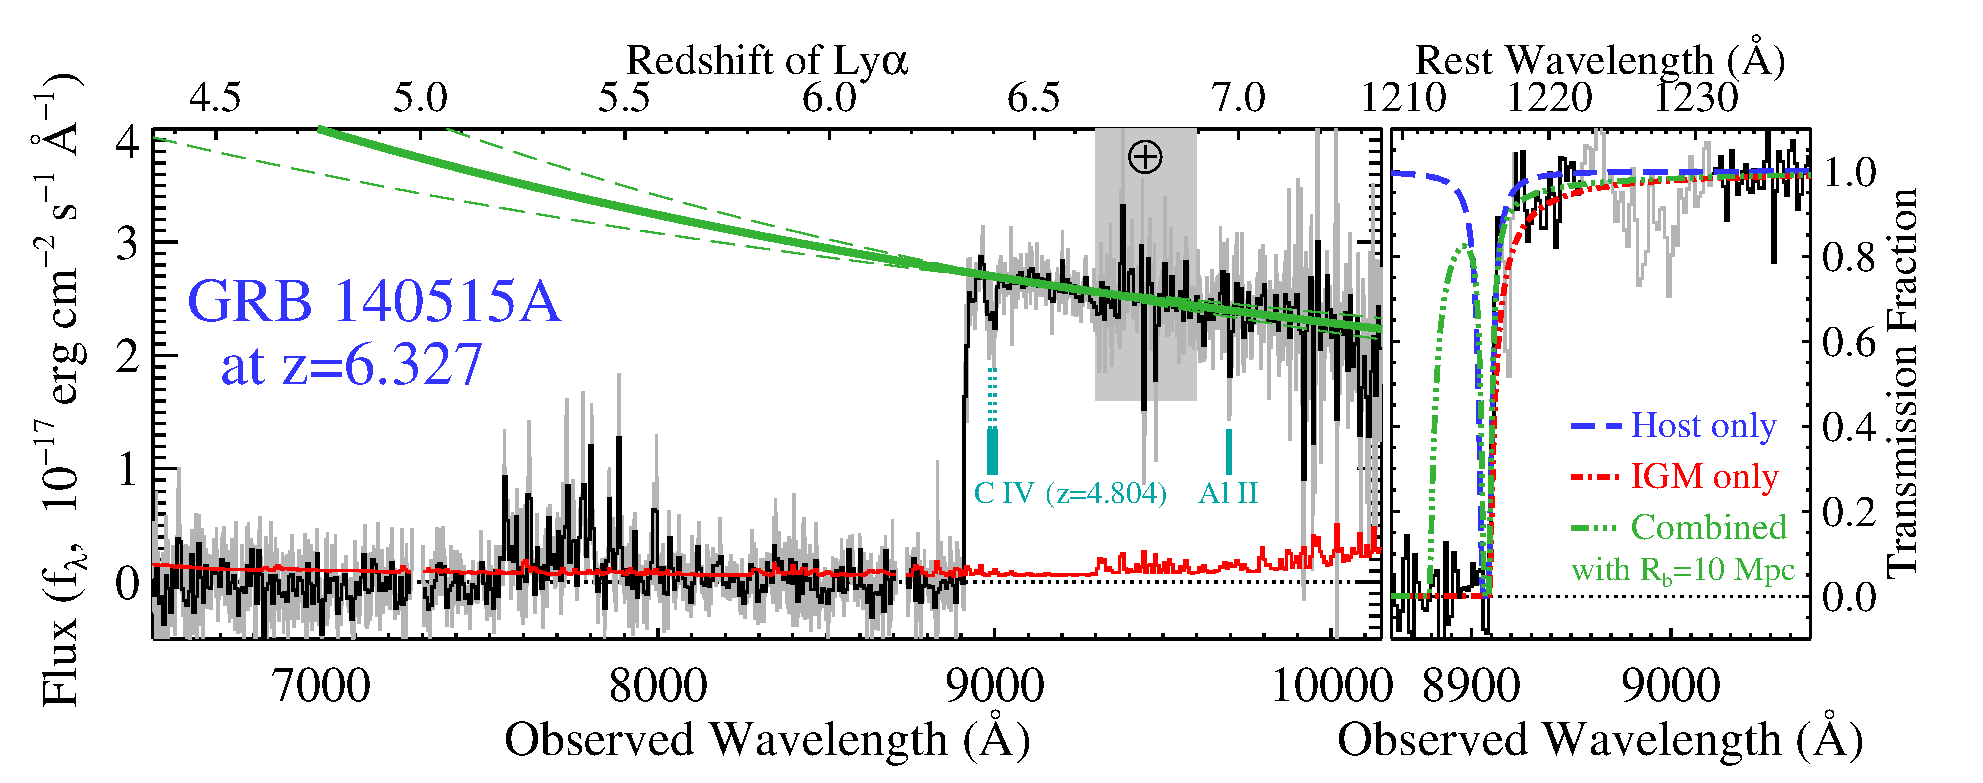
\includegraphics[width=14cm]{GRB140515A.eps}
  \caption{Spectrum of GRB140515A, a gamma-ray burst located at $z = 6.33$. The right-hand panel overlays damping wing models from a host absorber (blue), a pure IGM model with $\axhi = 0.056$ (red), and a combination model (green). The authors argue that, while each curve provides an equally-good fit to the data, the sharp rise in transmission shown is inconsistent with a significantly-neutral IGM. }
  \label{fig:GRB140515A}
\end{figure}


It is worth pointing out, however, that the method of searching for the damping wing redward of \lya\ is not without drawbacks. First, detecting the damping wing redward of \lya\ relies on your ability to understand what the quasar flux \textit{would have} been in the absence of the absorbing gas nearby the \lya\ line (this unabsorbed flux is referred to as the quasar \textit{continuum} and predicting the unabsorbed flux for a given quasar is called \textit{continuum fitting}). Predicting the \lya\ line properties in quasars is notoriously complicated and so modelling the precise fractional transmission must be done with care. Second, searching for the damping wing redward of \lya\ inherently involves measuring the gas properties nearby the quasar. However, quasars are extremely rare and special objects and it is not obvious that their surroundings are representative of the IGM on average. For example, \cite{Lidz:2007mz} found that quasars are likely born into large galaxy-generated ionized regions, suggesting that interpreting the \textit{lack} of a damping wing detection is not straightforward. Gamma-ray burst spectra are gaining attention in this regard (See \citealt{Salvaterra:2015gpa} for a review) as they tend to occupy more typical regions of space and have an easier-to-model continuum flux. The drawbacks of GRBs, though, is that they are often accompanied by a host absorber whose damping-wing absorption must be separated from that of the IGM. Third, even when provided with a clean detection of the damping wing redward of \lya, this will only tell you about one region of space and it will be difficult to use this single observation to extrapolate to the ionization state of the IGM as a whole. Later in this work, we propose a technique for searching for the hydrogen damping wing which, while faced with its own difficulties, is able to avoid the difficulties mentioned above. 

%Alternatively, the line profile for the hydrogen atom can be calculated classically by treating the electron as being harmonically-bound in the potential of the proton. The oscillations of the electron are intrinsically damped due to the fact that accelerating charges emit radiation. Furthermore, when we consider the probability of incident radiation being absorbed, the incident radiation can be seen as a driving force for the oscillator. 


% There is always a small damping of the oscillations by the radiation reaction force. I think this basically means that, since the charge is accelerating, it must be emitting radiation and losing energy and therefore its motion must be damped. Tau in this context is the time for radiation to cross a distance comparable to the size of the classical electron radius
\clearpage
\subsubsection{IGM Temperature}\label{sec:IntroIGMTemperature}

A detection of a damping wing redward of the \lya\ line in a quasar spectra would constitute a ``smoking gun" for significantly-neutral regions in the IGM, provided you could rule out the possibility of a DLA source. However, in the absence of a smoking gun, a \textit{warm} gun could be an indication of reionization having completed recently. Specifically, measurements of the IGM temperature can provide us with additional insights about the process of reionization. During reionization, patches of gas will be heated as they are ionized with their subsequent temperature only depending on the shape of the ionizing spectrum. Furthermore, once ionized, the thermal behavior of the gas is relatively simple: it will cool adiabatically as the Universe expands. Additional sources of heating, such as photo-heating from the ionization of the trace amounts of neutral hydrogen, and additional sources of cooling, such as Compton cooling off of CMB photons, will be insignificant. Because of this relatively simple cooling behavior, it should be possible to turn a measurement of the temperature of the IGM into a constraint on the timing of reionization. In order to do this, we need two main ingredients: a method of measuring the temperature of high-redshift gas and an understanding of how the temperature of the gas evolves with time after being ionized. 


One popular method for determining the temperature of the IGM utilizes the width of absorption lines in the \lya\ forest. In \S \ref{sec:IntroDampingWing}, we described the line profile for \lya\ absorption as obeying a Lorentzian distribution. While this is technically correct for any given atom, in reality, the atoms themselves have random thermal motions according to their temperature and will therefore see incident radiation as being redshifted or blueshifted accordingly.\footnote{The following discussion of Doppler broadening and the derivation of the Voigt profile closely follows notes taken from Masao Sako's ``Radiative Transfer" class offered in the Spring of 2010.}  As such, a hydrogen atom travelling \textit{toward} a photon with frequency just shy of the \lya\ frequency will see the light redshifted and can increase the chance of absorption. The effect of this is that the line profile for \lya\ absorption from a gas parcel gets smeared out, or, more precisely, gets convolved the with Maxwell-Boltzmann distribution. The greater the temperature, the greater the extent of this smearing. The Maxwell-Boltzmann distribution describes the velocities of particles in an ideal gas with a given temperature:


\begin{align}
W(\xi)\dd \xi &= \left( \dfrac{m_p}{2\pi k_{B}T} \right)^{1/2}e^{-m_p\xi^2/2 k_B T}\dd \xi \\
&= \left(\pi \xi_{0}^{2} \right)^{-1/2} e^{-\xi^{2}/\xi_{0}^{2}} \dd \xi \\
\xi_{0} &\equiv \sqrt{ \dfrac{2k_B T}{m_p}}
\end{align}


\begin{figure}[!p]
  \centering
  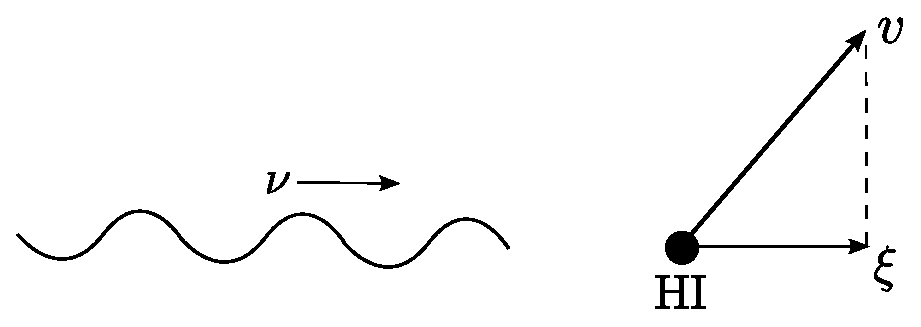
\includegraphics[width=8cm]{dopplerDiagram.eps}
  \caption{This diagram represents the process of Doppler broadening. The HI atom is moving away with velocity $v$ from incoming radiation with frequency $\nu$. The observed frequency of the radiation in the atom's rest frame is $\nu(1-\xi/c)$ where $\xi$ is the component of the velocity parallel with the incident radiation. }
  \label{fig:dopplerDiagram}
\end{figure}


where $T$ is the temperature of the gas, $\xi$ is the velocity and $k_{\text{B}}$ is the Boltzmann constant\gloss{$k_{\text{B}}$}{Boltzmann constant}Incident radiation will appear red/blueshifted in the frame of the absorbing atom with the shift being proportional to the atom's velocity \textit{parallel} to the incident radiation, as shown in Figure \ref{fig:dopplerDiagram}. Specifically, a photon with frequency $\nu$ will be observed by the atom to have frequency $\nu(1-\xi/c)$, where $\xi$ is the component of the atom's velocity \textit{away} from the incident radiation. Convolving our line profile with a Maxwell-Boltzmann distribution effectively involves replacing our expression in Eq. \ref{eq:IntroLineProfile} with

{\bf factors of $\lambda_{\alpha}??$}
\begin{align}
\sigma &\to \dfrac{\pi e^2}{m_e c}f_{\alpha}\lambda_{\alpha} \int_{-\infty}^{\infty} \dd \xi\ \phi(\nu(1-\xi/c)) W(\xi)\\
&= \dfrac{\pi e^2}{m_e c}f_{\alpha}\lambda_{\alpha} \int_{-\infty}^{\infty}\dd \xi\ \phi(\nu(1 - \xi/c)) \left(\pi \xi_{0}^{2} \right)^{-1/2} e^{-\xi^2/\xi_{0}^2} \\
&= \dfrac{\pi e^2}{m_e c} \frac{f_{\alpha}}{\pi} \left( \pi \xi_0^2 \right)^{-1/2} \int_{-\infty}^{\infty} \dd \xi \dfrac{(\Gamma/4\pi) e^{-\xi^2/\xi_{0}^{2}}}{(\nu-\nu_{0}(1-\xi/c))^2+(\Gamma/4\pi)^2}. \label{eq:IntroConvolution}
\end{align}

Here, we can make a couple substitutions and redefinitions:

\begin{align}
\Delta v_{\text{D}} &\equiv \nu_{0}\dfrac{\xi_{0}}{c} & y &\equiv -\xi/\xi_0 \\
v &\equiv \dfrac{\nu - \nu_{0}}{\Delta v_{\text{D}}} & a &\equiv \dfrac{\Gamma}{4\pi \Delta v_{\text{D}}}.
\end{align}

The quantity $\Delta v_{\text{D}}$ is known as the ``Doppler parameter" and is the red/blueshift in frequency space that the atom sees due to its thermal motion. The quantity $v$ is just the distance from line center in velocity space in units of the Doppler parameter. The quantity $a \equiv (\Gamma/4\pi)/\Delta v_{\text{D}}$ represents the ratio of the natural line width to the Doppler width. Rewriting our expression in Eq. \ref{eq:IntroConvolution}, we obtain

\begin{align}
\sigma(\nu) &= \dfrac{\pi e^2}{m_e c}f_{\alpha}\dfrac{1}{\sqrt{\pi}\Delta v_{\text{D}}} \dfrac{a}{\pi}\int_{-\infty}^{\infty}\dd y\ \dfrac{e^{-y^2}}{(v-y)^2+a^2}\\ 
&\equiv \dfrac{\sqrt{\pi} e^2}{m_e c} f_{\alpha}\dfrac{H(a,v)}{\Delta v_{\text{D}}}
\end{align}
where $H(a,v)$ is known as the Hjerting function \gloss{Hjerting Function}{Also known as the \textit{Voigt Function}, this function is commonly used in describing line profiles which incorporate Doppler broadening and the natural line width. This function is very relevant when studying the hydrogen damping wing.} or the Voigt function\gloss{Voigt Function}{Also known as the \textit{Hjerting Function}, this function is commonly used in describing line profiles which incorporate Doppler broadening and the natural line width. This function is very relevant when studying the hydrogen damping wing.}. So finally, we have obtained an expression for the \lya\ line profile incorporating the natural line width and Doppler broadening. Overall, the effect of the temperature acts to smear out the absorption line on scales of order $\sim 10\kms$ from line center. The greater the temperature, the larger the Doppler parameter and the greater the extent of the smearing. At scales $\gtrsim 100\kms$, the damping wing dominates the line profile. The profile is complex, but nonetheless, it encodes information about the underlying IGM temperature. Therefore, if simulations can generate accurate mock spectra for a variety of thermal histories, then comparisons between Voigt profile fits on the actual and mock spectra should be able to provide insight on the thermal properties of the IGM. 


This is the procedure undertaken by \cite{BoltonQuasar}. In Figure \ref{fig:QuasarProximityTemp}, they look for \lya\ absorption lines in the proximity zones of a high-redshift quasar in order to fit for the associated Doppler parameter and make inferences about the temperature. The top panel shows the fractional transmission for a mock quasar spectrum. The dashed curves indicate regions where absorption-line fitting was carried out and the vertical arrows indicate where the line centers were found from the fits. The second and third panel show the underlying temperature and density field, respectively. The bottom panel shows the true spectrum in question along with the same information regarding the line profile fits. These authors were able to use these fits to make inferences about the temperature of the IGM nearby the quasar. From these temperature measurements, and through comparison to mock spectra properties, these authors were able to place interesting limits on the ending of reionization ($z_{\text{H}} <  9$ assuming that the quasar reionizes its vicinity and Pop II stars drive reionization). This specific measurement is very difficult, however. The argument is essentially that the inferred temperature of the gas is too hot for reionization to have ended long before $z = 9$, otherwise the gas would have had more time to cool below the measured temperature. However, the regions nearby quasars should see a significantly-enhanced ionization field and all constraints made from measurements within this region hinge on ones ability to accurately account for such effects. 


The aforementioned technique for measuring the temperature is useful, but has the drawback that it requires the ability to detect \textit{individual absorption lines} in order to confidently fit a Voigt profile. However, at $z > 5$, it is no longer the case that absorption in the forest is due to isolated absorbers but is instead driven by density fluctuations in the diffuse IGM. As such, individual absorption features blend together and the forest becomes somewhat inverted where, instead of stretches of transmission being punctuated with absorption features, stretches of absorption are punctuated with transmission features. This renders the goal of fitting for individual Voigt profiles impossible in the IGM. This also explains why \cite{BoltonQuasar} analyze the IGM  nearby a high-redshift quasar, where the transmission is enhanced due to the strengthened ionization field. 


An alternative approach to fitting line profiles is to measure the small scale power of the flux fluctuations (e.g., \citealt{Lidz2010}, \citealt{Theuns2002a}, \citealt{zaldarriaga2002searching}). This involves applying a localized wavelet filter to measurements of the \lya\ forest in order to measure the level of small-scale fluctuations. As we mentioned, large temperatures will lead to a larger Doppler parameter which will smear out small-scale structure. Thus, a large response to a small-scale wavelet filter would indicate significant small-scale structure and suggest a lower temperature for the gas. This approach has the important advantage that it doesn't rely on individual absorption lines to be discernible in order to extract temperature measurements. In \S \ref{sec:IGMTemperature}, we show that this can be used to constrain the IGM temperature at $z > 5$, \textit{even in typical regions of the IGM}.

%% Maybe we can defer discussion of this equation to chapter 3?
%\begin{align}
%\dfrac{\dd T}{\dd t} &= -2HT + \dfrac{2T}{3(1+\delta)}\dfrac{\dd \delta}{\dd t} + \dfrac{T}{\mu} \dfrac{\dd \mu}{\dd t} + \dfrac{2\mu m_p}{3\rho k_B}(\mathcal{H} - \Lambda) \label{eq:dtdt}
%\end{align}

\begin{figure}[!p]
  \centering
  \includegraphics[width=11cm]{BoltonIGMTemperature_Fig2.ps}
  \includegraphics[width=11cm]{BoltonIGMTemperature_Fig2b.ps}
  \caption{This figure shows mock spectra, and corresponding simulated IGM properties, from \cite{BoltonQuasar} in the top four panels. The bottom panel shows the observed spectrum from SDSS J0818+1722, which \cite{BoltonQuasar} use in order to make temperature measurements inside the proximity zone. Dashed lines indicate regions where Voigt-profile fitting was performed and downward arrows indicate the detected centers of the Voigt profiles.}
  \label{fig:QuasarProximityTemp}
\end{figure}

\clearpage
\subsubsection{Motivation for this Work}

This discussion of the \lya\ forest as a tool for constraining the EoR highlights several of the current drawbacks of the approach. Among these, the largest is arguably the degeneracy between different sources of saturated absorption in the \lya\ forest. If one could find a way to determine if absorption in the \lya\ forest was certainly happening as a result of underlying neutral hydrogen, then it would be easier to interpret observations in terms of the overall neutral fraction of the Universe. We highlighted one example of how this has been done: the hydrogen damping wing redward of \lya. While a useful approach, this also suffers from drawbacks of its own, namely the limited number of high-redshift spectra suitable for damping-wing searches and the fact that regions surrounding quasars are not expected to be representative of the IGM as a whole. This helps motivate two approaches we consider in \S \ref{sec:NeutralIslands}. Namely, we identify the hydrogen damping wing and absorption due to deuterium as ``smoking gun" signals of underlying hydrogen and search for them in typical regions of the IGM. Obviously, it will become clear that this approach suffers from its own drawbacks but it does provide an independent measurement useful for constraining the ionization state of the high-redshift IGM.

Second, we have discussed some difficulty in making measurements of the temperature of the high-redshift IGM. Namely, due to the high levels of absorption in the \lya\ forest of quasar spectra at these redshifts, traditional methods of inferring the IGM temperature are inapplicable except in the highly-complex near-zones of quasars. This motivates the development of a temperature-measurement technique which is applicable to typical regions of the high-redshift IGM. Such a technique is proposed in {\bf cite} and discussed in \S \ref{sec:IGMTemperature}.

\clearpage
\subsection{The 21-cm Line}\label{sec:21cm}

The 21-cm line refers to the hyperfine splitting of the hydrogen atom where, due to the interaction between the magnetic dipole moments\gloss{Magnetic Dipole Moment}{The magnetic dipole moment of an object is related to the torque it would experience when placed in an external magnetic field. Magnetic moments are often relevant for bar magnets or loops of current. In the context of the hydrogen atom, the spin of the proton and electric render them as a sort of ``loop of current'' which gives them their own magnetic dipole moment.} of the electron and proton, a small energy difference exists between the configuration where the spins of the electron and proton are aligned versus where they are anti-aligned. The configuration where the spins are anti-aligned (and magnetic dipole moments are therefore aligned) is energetically favored and has a lower energy by $\Delta E \approx 6\times 10^{-6}$eV.\footnote{This is in contrast to a \lya\ photon which has energy $E \approx 10.2\text{eV}$, more than a million times greater.} Thus, spin-flip transitions will result in (from) the emission (absorption) of a photon with $\lambda \approx 21\cm$, $\nu \approx 1420\mhz$. This is shown schematically in Figure \ref{fig:21cmline}. 

%However, the 21-cm transition is a ``forbidden'' transition\gloss{Forbidden Transition}{This refers to atomic transitions which are not allowed under the quantum mechanical selection rules under the dipole approximation. Essentially, this means the transitions are relatively extremely rare compared to ``allowed'' transitions.}, meaning its rate of occurrence is extremely low. As a result,

As we discussed in \S \ref{sec:LyaForest}, the cross section or the \lya\ transition is extremely large, which presents us with a host of difficulties.  However, the Universe is essentially transparent to 21-cm photons, allowing them to travel unimpeded from distant neutral hydrogen to us. In principal, this allows us to observe the hydrogen density field directly up to redshifts of $z \sim 150$, \textit{far beyond the timescale of reionization} and far beyond the reach of the \lya\ forest. Measurements of the evolution of the 21-cm signal with redshift would allow us to construct something like a reionization ``movie'', which would constitute the ultimate constraint on reionization. 


Mapping the intensity of the 21-cm line during reionization avoids many other drawbacks of the \lya\ line as well. Namely, intensity mapping would provide us with a 3D volume of intensity values, as opposed to the \lya\ forest which is typically observed one sightline at a time. Also, since we are directly observing the hydrogen, interpretation of observations of the 21cm signal will be significantly simplified.

In this section, let us start with a overview of the physics of the 21-cm line and then continue by discussing a couple avenues by which the 21-cm signal could be utilized in order to constrain reionization. 

\clearpage
\subsubsection{The Intensity of the 21-cm Line}\label{sec:21cmPhysics}


Let us start by considering the brightness of 21-cm emission from a distant hydrogen gas cloud.\footnote{This discussion will closely follow \S 2.1 of \citealt{Furlanetto2006}, which is an excellent review of the 21-cm line.} This is usually described in terms of a \textit{specific intensity} and then in terms of a \textit{brightness temperature}\gloss{Brightness Temperature ($T_b(\nu)$)}{An object with a given specific intensity $I_{\nu}$ has a corresponding brightness temperature equal to the requisite temperature of a blackbody for its specific intensity to equal that of the object, $I_{\nu} = B_{\nu}(T_{b}(\nu))$.}\gloss{Specific Intensity ($I_{\nu}$)}{The specific intensity of light leaving a cloud of gas is the energy carried by the light per unit frequency, area, time, and solid angle.}. The specific intensity of light leaving our HI cloud is the amount of energy per unit frequency, time, area, and solid angle, denoted $I_{\nu}$. The brightness temperature is the required temperature of a blackbody to radiate with the same specific intensity at that frequency, i.e., $B_{\nu}(T_b) = I_{\nu}$, where $B_{\nu}$ denotes the blackbody spectrum. 


The light we observe from our HI cloud will be a combination of background light shining \textit{through} the cloud and light emitted by the cloud itself. This follows the radiative transfer equation (in the clouds frame)

\begin{align}
T_b(\nu) &= T_{\text{cloud}}(1-e^{-\tau_{\nu}}) + T_{\text{background}}e^{-\tau_{\nu}} \label{eq:cloudframe}
\end{align}
where the background light is from the CMB, such that $T_{\text{background}} = 2.73\text{K}(1+z)$, and $T_{\text{cloud}}$ is the \textit{spin temperature} of the cloud, defined below. The quantity $\tau_{\nu}$ is the frequency-dependent optical depth for absorption \textit{by} the HI cloud. This is equal to 

\begin{align}
\tau_{\nu} &= \int \dd s \sigma_{01}\left( 1 - e^{-E_{10}/k_{\text{B}}T_{\text{S}}} \right) \phi(\nu) n_{0} \label{eq:tau21}
\end{align}

where the integral is carried out along the line of sight through the cloud. In this expression, $E_{10} \approx 6\times 10^{-6}$eV is the energy of the transition, $\phi(\nu)$ is the line profile, $\sigma_{01}$ is the cross-section for 21-cm absorption by a hydrogen atom and $n_{0}$ is the number density of hydrogen atoms in the unexcited state. We follow the convention of \cite{Furlanetto2006} and denote the lower energy level by ``0'' and the higher energy level by ``1''. The ratio of the population of atoms in the excited state to the ground state is defined by the spin temperature and the degeneracy of the states:

\begin{align}
\dfrac{n_{1}}{n_{0}} &= \dfrac{g_1}{g_0}e^{-E_{10}/k_{\text{B}}T_{\text{S}}} = 3 e^{-E_{10}/k_{\text{B}}T_{\text{S}}}.
\end{align}

The excited state is the triplet state and has a three-fold degeneracy: $|\uparrow \uparrow \rangle$, $\dfrac{1}{\sqrt{2}}(|\uparrow \downarrow\rangle + |\downarrow \uparrow \rangle)$, $|\downarrow \downarrow\rangle$, and the lower-energy state is the singlet state: $\dfrac{1}{\sqrt{2}}( |\uparrow \downarrow\rangle - |\downarrow \uparrow \rangle)$, where arrows denote the spin. $T_{\text{S}}$ is the spin temperature and is defined via this equation. For our purposes, $T_{\text{S}} \gg E_{10}/k_{\text{B}}$, so we have $n_{1}/n_{0} = 3$ and

\begin{align}
1 - e^{-E_{10}/k_{\text{B}}T_{\text{S}}} &\approx \dfrac{E_{10}}{k_{\text{B}}T_{\text{S}}}.
\end{align}


 Furthermore, the integral along the line of sight of the number density of hydrogen atoms in the hyperfine ground state will simply be the column density of hydrogen atoms multiplied by 1/4, $N_{\text{HI}}/4$. Here, the factor of $\frac14$ accounts for the fact that only one out of four hydrogen atoms will be in the singlet state on average. Putting this together, Eq. \ref{eq:tau21} becomes
 
\begin{align}
\tau_{\nu} &\approx \sigma_{01} \dfrac{N_{\text{HI}}}{4} \dfrac{E_{\text{10}}}{k_{\text{B}}T_{\text{S}}} \phi(\nu)
\end{align}
where 
\begin{align}
\sigma_{01} &\equiv \dfrac{3c^2 A_{10}}{8\pi\nu^{2}}
\end{align}

is the cross section for 21-cm absorption and $A_{10} = 2.85 \times 10^{-15}\sec^{-1}$ is the spontaneous emission coefficient for the transition and $\phi(\nu)$ is the 21-cm line profile. As we discussed in \S \ref{sec:IntroIGMTemperature}, line profiles depend on several properties of the gas, however, here it is the case that Doppler broadening due to the expansion of the Universe dominates the line profile, such that

\begin{align}
\phi(\nu) \approx \dfrac{c}{s H(z) \nu}
\end{align}

where $s$ is the proper distance between two points expanding away from each other. Putting these pieces together, our expression for the optical depth becomes:

\begin{align}
\tau_{\nu} &\approx \dfrac{3c^2 A_{10}}{8\pi \nu^{2}} \dfrac{h \nu}{k_{\text{B}}T_{\text{S}}} \dfrac{c}{s H(z) \nu} \dfrac{n_{\text{HI}}\langle x_{\text{HI}}\rangle s}{4} \tag{$N_{\text{HI}} = s n_{\text{HI}}\axhi$}\\
&\approx \dfrac{3hc^3 A_{10}}{32\pi \nu^2 k_{\text{B}}T_{\text{S}}} \dfrac{n_{\text{HI}}\axhi}{H(z)}
\end{align}
plugging in values and evaluating at line center, \cite{Furlanetto2006} obtain

\begin{align}
\tau_{\nu_{0}} &\approx 0.0092 (1+\delta)(1+z)^{3/2}\dfrac{\axhi}{T_{\text{S}}}\left[ \dfrac{H(z)/(1+z)}{\dd v_{\parallel}/\dd r_{\parallel}} \right] 
\end{align}

where $\dd v_{\parallel}/\dd r_{\parallel}$ is the gradient in the line-of-sight velocity (peculiar velocity and velocity due to Hubble expansion) and the ratio of that with $H(z)/(1+z)$ represents the deviation from pure-Hubble expansion. For the purposes of the 21-cm probes we will discuss, we actually care about the \textit{contrast} between the 21-cm signal and the background CMB signal. Thus, the relevant brightness temperature contrast, in our frame, is 

\begin{align}
\delta T_{b} &= \dfrac{1}{1+z}\left[ T_{\text{S}}(1-e^{-\tau_{\nu_{0}}}) + T_{\text{CMB}}e^{-\tau_{\nu_{0}}} - T_{\text{CMB}} \right] \\
&= \dfrac{T_{\text{S}}-T_{\text{CMB}}}{1+z} (1 - e^{-\tau_{\nu_{0}}}) \\
&\approx \dfrac{T_{\text{S}}-T_{\text{CMB}}}{1+z} \tau_{\nu_{0}} \\ 
&\approx 9\text{mK}\cdot x_{\text{HI}}(1+\delta)(1+z)^{1/2}\left[ 1 - \dfrac{T_{\text{CMB}}}{T_{\text{S}}} \right] \left[ \dfrac{H(z)/(1+z)}{\dd v_{\parallel}/ \dd r_{\parallel}} \right] \\ 
&\approx 24 \text{mK}\cdot x_{\text{HI}}(1+\delta)\left(\frac{1+z}{7}\right)^{1/2}\left[ 1 - \dfrac{T_{\text{CMB}}}{T_{\text{S}}} \right] \left[ \dfrac{H(z)/(1+z)}{\dd v_{\parallel}/ \dd r_{\parallel}} \right]. \label{eq:dTb}
\end{align}

Thus, we see that a neutral parcel of hydrogen at mean density and $z = 6$ and $T_{\text{S}} \gg T_{\text{CMB}}$, the brightness temperature contrast is $\sim 24\text{mK}$. 


\begin{figure}[!p]
  \centering
  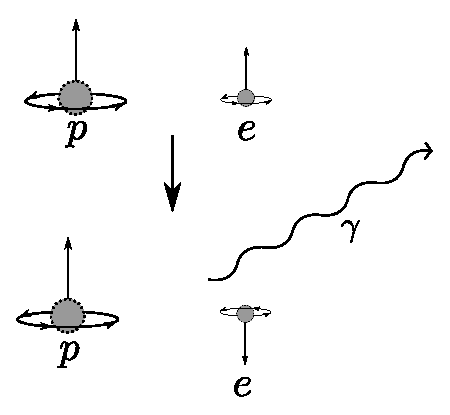
\includegraphics[width=8cm]{21cmline.eps}
  \caption{Schematic representation of the 21-cm transition where the transition between aligned spins of the proton and electron to anti-aligned spins results in the emission of a photon with $\lambda \approx 21$cm. }
  \label{fig:21cmline}
\end{figure}

\begin{figure}[!p]
  \centering
  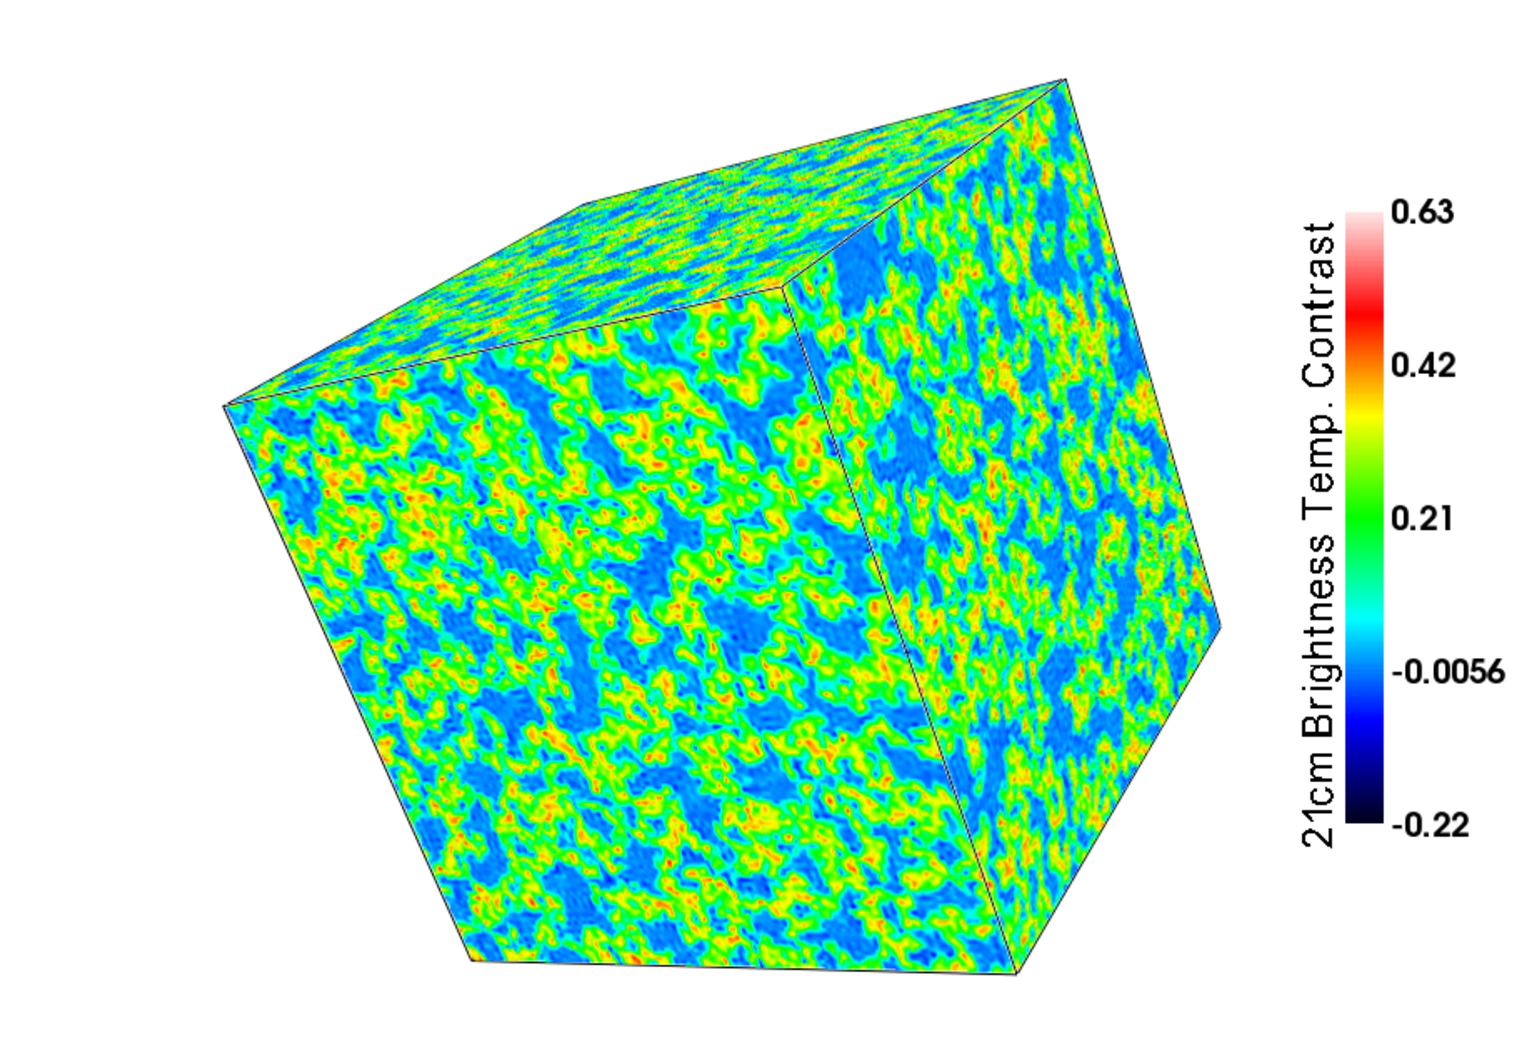
\includegraphics[width=8cm]{TalkSignal.eps}
  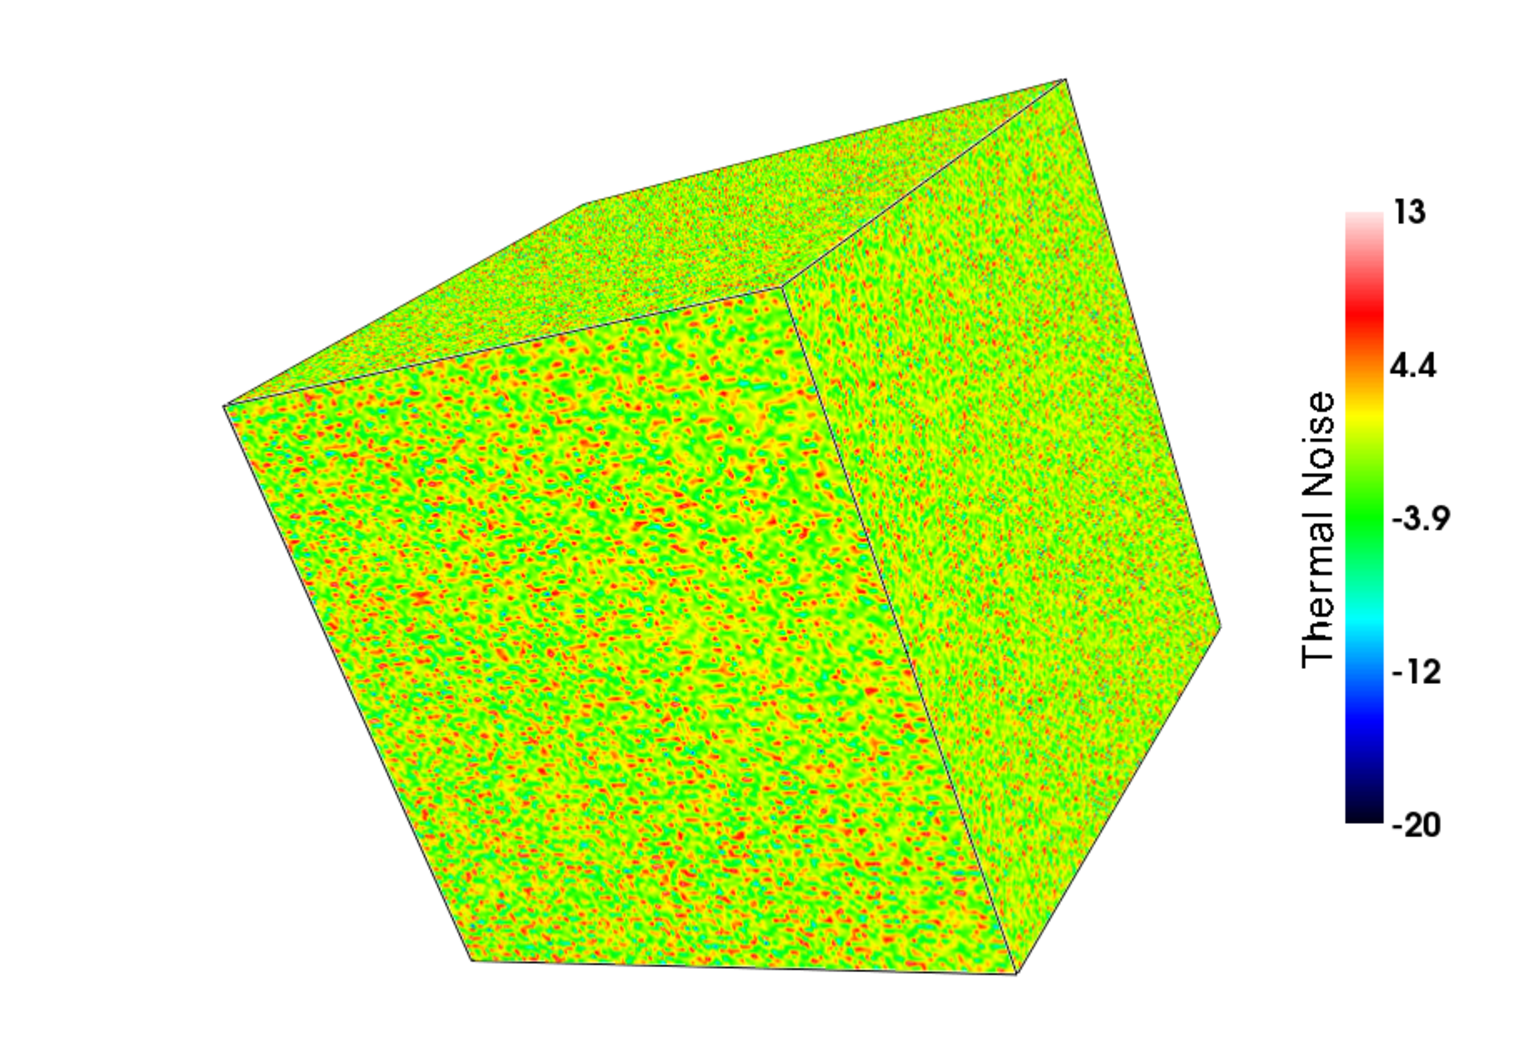
\includegraphics[width=8cm]{TalkNoise.eps}
  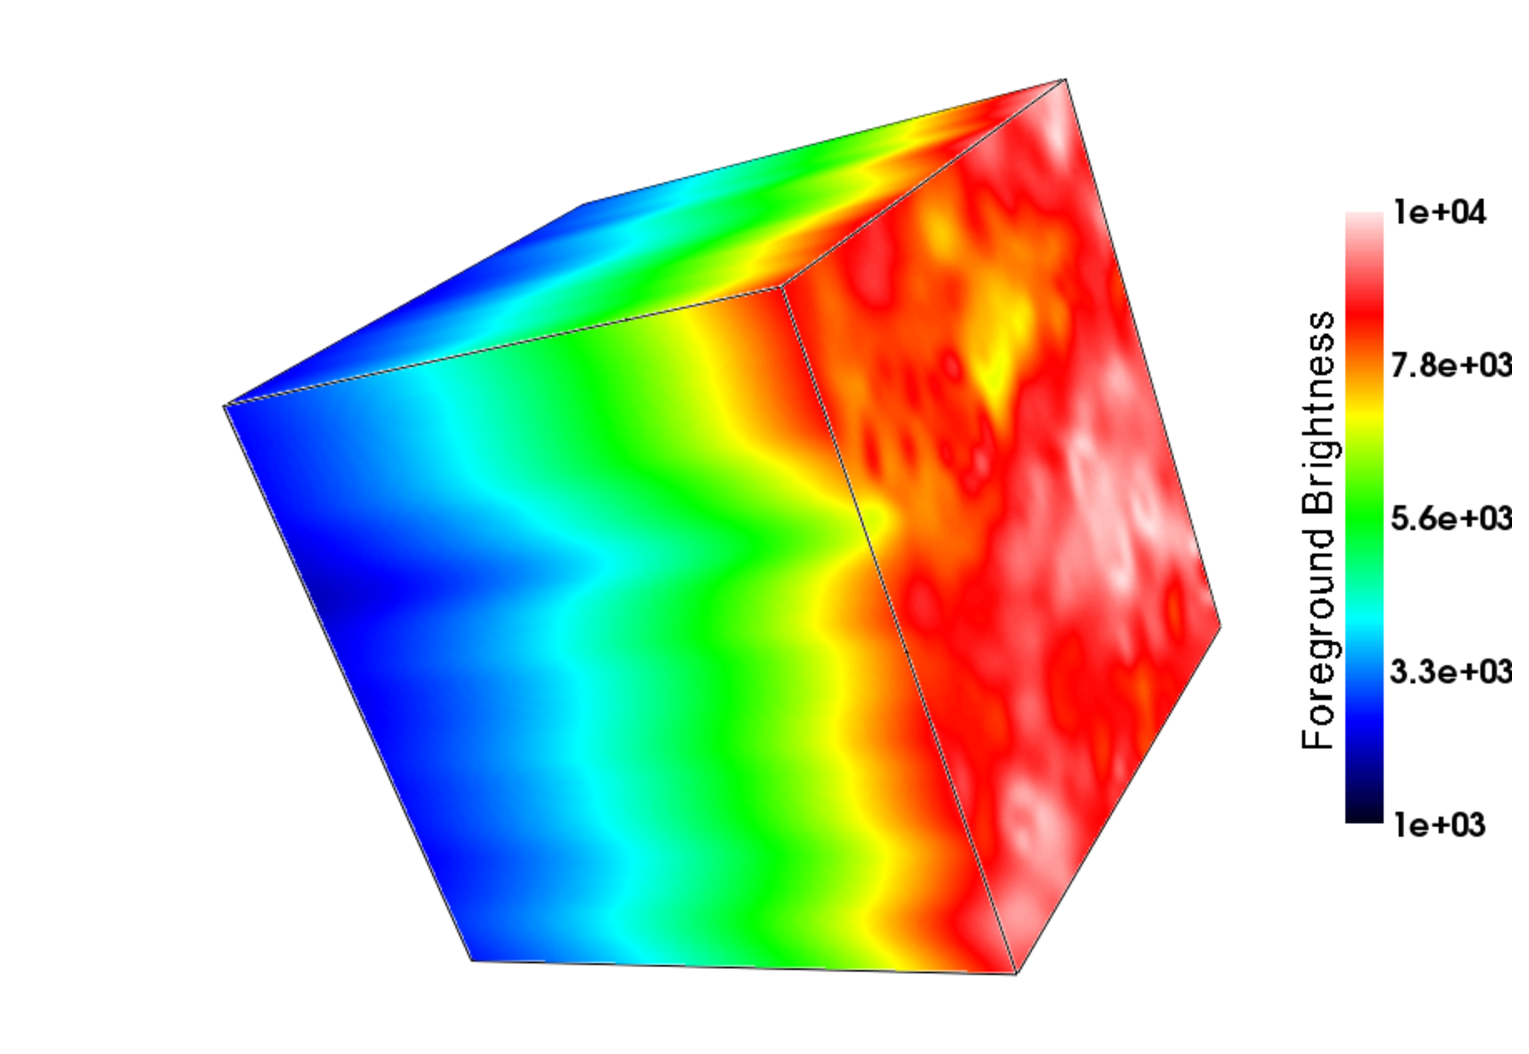
\includegraphics[width=8cm]{TalkFG.eps}
  \caption{Simulation cube of the 21-cm signal during reionization (top) along with simulated noise for an interferometer (middle) and the galactic foregrounds (bottom). This figure demonstrates that, while the sources of noise are several orders of magnitude larger than the signal, these three contributions to observations are dominant of different scales. The volume of each cube is 1 $(\text{Gpc}/h)^{3}$. In this figure, the line of sight direction away from the observer is to the right and slightly out of the page. }
  \label{fig:21cmCube}
\end{figure}

\clearpage
\subsubsection{21-cm Fluctuations with Interferometers}\label{sec:21cmFluctuations}


The first approach for utilizing the 21-cm line in order to learn about reionization that we will discuss is through the use of 21-cm fluctuations. The ultimate goal for the 21-cm line for people interested in reionization is to image the 21-cm intensity field for the duration of reionization. Since the 21-cm radiation of interest is emitted at $z \approx 10$, by the time it arrives to us, its wavelength will have redshifted to $\sim 2\meter$. Thus, observations of 21-cm fluctuations must be made with large interferometers, consisting of tens to thousands of antennae, and maximum separations (baselines) of the order 1 km. 

Before continuing, it may be helpful to provide a brief description of what interferometry is, for which we will follow \cite{morales2009reionization}. Interferometers are built of many antennae which observe the electric field at their location and correlate those measurements to image the sky. Let us consider a single antenna which observes a time-and-angle-dependent electric field, defined $E(\theta,t)$. A nearby antenna, separated from the first by the vector $\vec{r}$, will observe a similar electric field, but the field will have a phase shift owing to the difference in path length that the radiation had to travel between going to the first and the second antennae. If we are observing directly overhead, then light will have to travel an equal distance to reach either antenna. Conversely, if we are observing at the horizon along the line connecting the antennae, then it will take light extra time to reach one of the antenna opposed to the other ($\Delta t = |\vec{r}|/c$). This is illustrated in Figure \ref{fig:interferometry}. Based on this figure, we can see that the extra path length for the light will be 

\begin{align}
\Delta \ell &= \vec{r}\cdot\hat{\theta}
\end{align}

resulting in a \textit{phase difference} of 

\begin{align}
\Delta \phi &= 2\pi \frac{\vec{r}\cdot\hat{\theta}}{\lambda}.
\end{align}


Therefore, if the first antenna sees an electric field $E(\theta,t)$, then the second antenna will see $E_2(\theta,t) = E(\theta,t)e^{-2\pi i (\vec{r}\cdot{\theta}/\lambda)}$. Therefore, the observed electric field at any position, $\vec{r}$, is related to that at the first antenna by

\begin{align}
E(\vec{r},\theta,t) &= E(\theta,t)e^{-2\pi i (\vec{r} \cdot \hat{\theta}/\lambda)}.
\end{align}

If we integrate over the entire sky, we find

\begin{align}
E(\vec{r},t) &= \int \dd^{2} \theta E(\theta,t) e^{-2\pi i (\vec{r}\cdot \hat{\theta}/\lambda)}.
\end{align}

However, the expression on the right appears very familiar to us since it is simply a Fourier transform. Therefore, we see that the observed electric field on the surface of the Earth is actually just a Fourier transform\gloss{Fourier Transform}{A Fourier transform essentially describes a function as a weighted sum of infinitely many sine waves with different frequencies. The Fourier transform describes the weights of the different sine curves and therefore gives information about the relevant distances scales in your function.} of the electric field on the surface of the sky. This is basically what allows measurements at many locations on the ground to be converted into measurements of the 21-cm signal across the sky. Furthermore, each pair of antenna essentially measure a particular Fourier \textit{mode}, $k$, on the sky:

\begin{align}
{\bf k} &= \frac{2\pi {\bf u}}{D}\label{eq:modes}
\end{align}

where ${\bf u}$ denotes the separation of a pair of antenna in units of the observed wavelength, $D$ is the co-moving distance to the source of the emission, and ${\bf k}$ is akin to a spatial frequency at the location of the emission. Thus, this demonstrates that many measurements on the ground can give us information of the 21-cm signal as a function of position on the sky, with widely-separated antenna providing information on \textit{small scales} and closely-separated antenna providing information on the large scales. Several experiments are currently planned or underway with the goal of measuring this signal. These include the Precision Array for Probing the Epoch of Reionization (PAPER, \citealt{Parsons2012}, underway), the Murchison Widefield Array (MWA, \citealt{Tingay2012}, underway), the Hydrogen Epoch of Reionization Array (HERA\footnote{{\tt http://reionization.org/}}, planned), the Square Kilometer Array (SKA\footnote{{\tt https://www.skatelescope.org/}}, scheduled construction 2018), the Low Frequency Array (LOFAR, \citealt{2013A&A...550A.136Y}, underway), and the Giant Metrewave Radio Telescope (GMRT, \citealt{Paciga2011}, underway). These experiments are further discussed in \S \ref{sec:21cmExperiments}.


However, before these experiments can uncover the cosmological 21-cm signal, they must first overcome several formidable sources of noise. Synchrotron emission\gloss{Synchrotron Radiation}{Radiation emitted by charged particles undergoing radial acceleration, such as in synchrotron particle accelerators. This constitutes a significant source of noise for 21-cm observations.}, free-free emission\gloss{Free-Free Emission}{Emission from a charged particle that is free both before and after the interaction. Examples include electrons in an ionized hydrogen cloud interacting with protons without being captured.}, and Bremsstrahlung radiation\gloss{Bremsstrahlung Radiation}{Emission from charged particles undergoing acceleration due to interactions with other charged particles. Literally translates to ``braking radiation''.} from our own galaxy constitute the largest nuisance at the frequencies of interest ($\nu \approx 140\mhz$) in sheer magnitude. In a relatively ``cold'' spot on the sky, \cite{Furlanetto2006} state that the intensity of this radiation obeys the following scaling relation:

\begin{align}
T_{\text{sky}} \sim 180 \left( \dfrac{\nu}{180\mhz} \right)^{-2.6}\kelvin, \label{eq:Tsky}
\end{align}

which scales to $T_{\text{sky}} \sim 130\kelvin$ at $z = 6$. Thus, we see in this specific example, the intensity of the foreground emission from our galaxy should be $\gtrsim 5000$ times greater than the 21-cm signal itself. Furthermore, while it is often the case that sources of noise can be beaten down with increased observation time, these galactic foregrounds are a permanent feature of the sky.  While this presents an enormous challenge for observing the 21-cm signal from the EoR, not all hope is lost. 


We can see from Eq. \ref{eq:Tsky} that the foreground noise from the galaxy should vary very \textit{smoothly} with frequency. Meanwhile, for the 21-cm signal, slight decreases in observed frequency are equivalent to observing the 21-cm signal from a more distant point in space. For example, in the case of ionized bubbles of size $\ell \approx 10\mpch$, we would expect fluctuations of 100\% in the 21-cm signal over this distance. However, this distance at a redshift of $z \approx 7$ corresponds to a frequency change of $\Delta \nu \approx 1\mhz$ and a  (relatively predictable) change in the amplitude of the foreground signal of only $\lesssim3\%$. This is further demonstrated by Figure \ref{fig:21cmCube}. The top cube shows what the 21-cm signal would look (in arbitrary units) like for a 1Gpc/$h$ cube of the Universe from a reionization simulation. We can see bubbles of size $\sim10\mpch$ and therefore fluctuations in the 21-cm signal on that scale. In the bottom panel, we show a simulation of the galactic foregrounds (provided by Piyanat Kittiwisit at ASU) corresponding to the same physical region in space. In this case, the dimension of the cube that goes to the right and slightly out of the page is the line of sight direction away from us. We see that, along this direction, the foreground emission varies very smoothly, as expected from Eq. \ref{eq:Tsky}. Thus, in principle, the contributions to the observed signal from the EoR and from the galaxy should separable. This is essentially done by removing large-scale modes from the observed signal, as briefly discussed in \S \ref{sec:Bubbleforegrounds}.



\begin{figure}[!p]
  \centering
  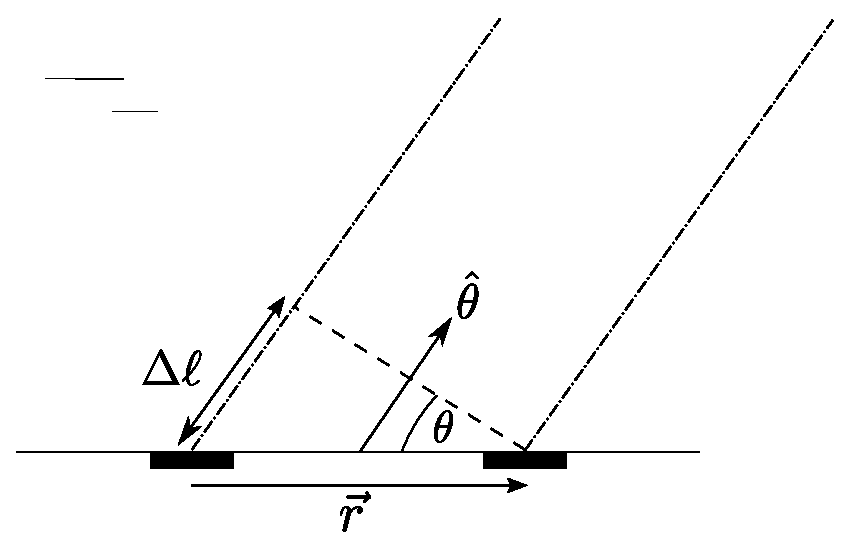
\includegraphics[width=8cm]{interferometry.eps}
  \caption{This figure depicts the extra path length, $\Delta \ell$, of radiation (dot-dashed lines) incident on two elements (solid black rectangles) in an array separated by $\vec{r}$ when considering a position on the sky $\hat{\theta}$.}
  \label{fig:interferometry}
\end{figure}


A second significant source of noise is thermal noise from the experiment itself. This is discussed in more detail in \S \ref{sec:Bubblenoise}, but the power spectrum for the noise should follow (\citealt{McQuinn2006},\citealt{Furlanetto2006})

\begin{align}
P_{\text{N}} &= \dfrac{T_{\text{sky}}^{2}}{B\ t_{\text{int}}} \dfrac{D^{2}\Delta D}{n(k_{\perp})}\left( \dfrac{\lambda^{2}}{A_{\text{e}}} \right)^{2}.
\end{align}

Here, $k_{\perp}$ is the component of ${\bf k}$ transverse to the line of sight, $B$ is the bandwidth of the observation, $t_{\text{int}}$ is the integration time for the experiment, $n(k_{\perp})$ is the number density of baselines observing the specific wavemode, $\Delta D$ is the depth of the observation field, and $A_{\text{e}}$ is the effective collecting area per tile. With the exception of $T_{\text{sky}}$ and $\lambda$ and $D$, these are controllable parameters of the experiment. This allows for several avenues toward beating down the thermal noise, the most popular of which are through increasing observation time, re-arranging tiles in order to alter $n(k_{\perp})$, and increasing collecting area. Thus, unlike the galactic foregrounds, the thermal noise is a nuisance which will become less and less important as experiments evolve. 


For the first generation of experiments, however, the levels of thermal noise should prevent the 21-cm signal from being mapped and prevent any reionization ``movies'' from being made. This is discussed in \cite{McQuinn2006} and shown in Figure \ref{fig:McQuinnSNR}. Specifically, this figure shows the fraction of pixels at each $k$ which will be imaged (have $\text{SNR} \geq 1$) for MWA (dashed), LOFAR (dot-dashed), and SKA (solid) assuming galactic foregrounds can be subtracted. With regard to foregrounds, though, it is likely that any $k$ modes below the vertical hatched line will be inaccessible due to residuals from the foreground subtraction. This demonstrates that, due to thermal noise, first-generation interferometers like the MWA and LOFAR will image a small fraction of the pixels at the $k$ modes unspoiled by foregrounds and will therefore be unable to make maps of the 21-cm sky during reionization.\footnote{This estimate is done assuming that fluctuations in the 21-cm signal are caused by density fluctuations rather than by fluctuations in the ionization field. The latter should lead to a larger signal and so, in this sense, this estimate is somewhat pessimistic. The general point still holds, however.} 

\begin{figure}[!p]
  \centering
  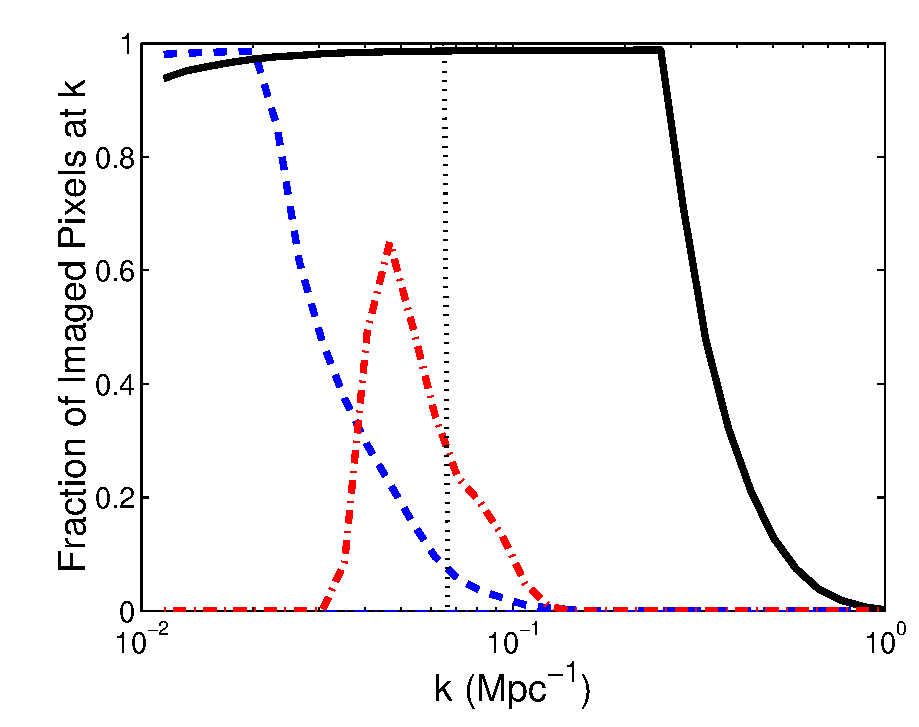
\includegraphics[width=8cm]{McQuinnSNR.eps}
  \caption{This figure shows the percentage of pixels ``imaged'' ($\text{SNR} > 1$) as a function of wavemode, $k$ for the MWA (dashed), LOFAR (dot-dashed), and the SKA (solid). The vertical hatched line shows the distance scale above with (smaller $k$) the residuals from foreground subtraction are expected to dominate the 21-cm signal. This demonstrates that, for first-generation 21-cm experiments, a very small fraction of pixels with $k > k_{\text{hatched}}$ will be ``imaged''. This estimate assumes that fluctuations in the 21-cm signal are driven from density fluctuations rather than fluctuations in the ionization field, so it is somewhat conservative. Taken from \cite{McQuinn2006}. }
  \label{fig:McQuinnSNR}
\end{figure}


In Figure \ref{fig:21cmCube} we show a random, qualitatively-representative simulated realization of thermal noise. While this panel indeed does demonstrate that thermal noise should dominate the 21-cm signal (top) in sheer magnitude, it also demonstrates that the fluctuations in the thermal noise are expected to happen on scales \textit{smaller} than those in the 21-cm signal. While galactic foregrounds ruin large-scale modes, and thermal noise ruin small-scale modes, an intermediate region of $k$-space should remain accessible to the interferometers. It will not be the case that first-generation interferometers can image or make movies of the 21-cm signal, but they still may learn about how the signal behaves on different physical scales, i.e. the \textit{power spectrum}, and how that behavior evolves with redshift. 


In fact, \cite{Lidz2008} investigate the evolution of the power spectrum throughout reionization under several simulated reionization scenarios. They find that a generic result to all the models is that the \textit{slope} of the power spectrum, in the accessible $k$-mode range ($0.1\ h/\text{Mpc} \leq k \leq 1\ h/\text{Mpc}$) should \textit{decrease} as reionization evolves. Meanwhile, the \textit{amplitude} of the power spectrum in this $k$-mode range should rise until reionization reaches its midpoint and then fall. Thus, measuring the 21-cm power spectrum at several redshifts and confirming this behavior can, first, increase our confidence that we are in fact observing the 21-cm signal from reionization and, second, help us learn about the reionization process itself. 

\begin{figure}[!p]
  \centering
  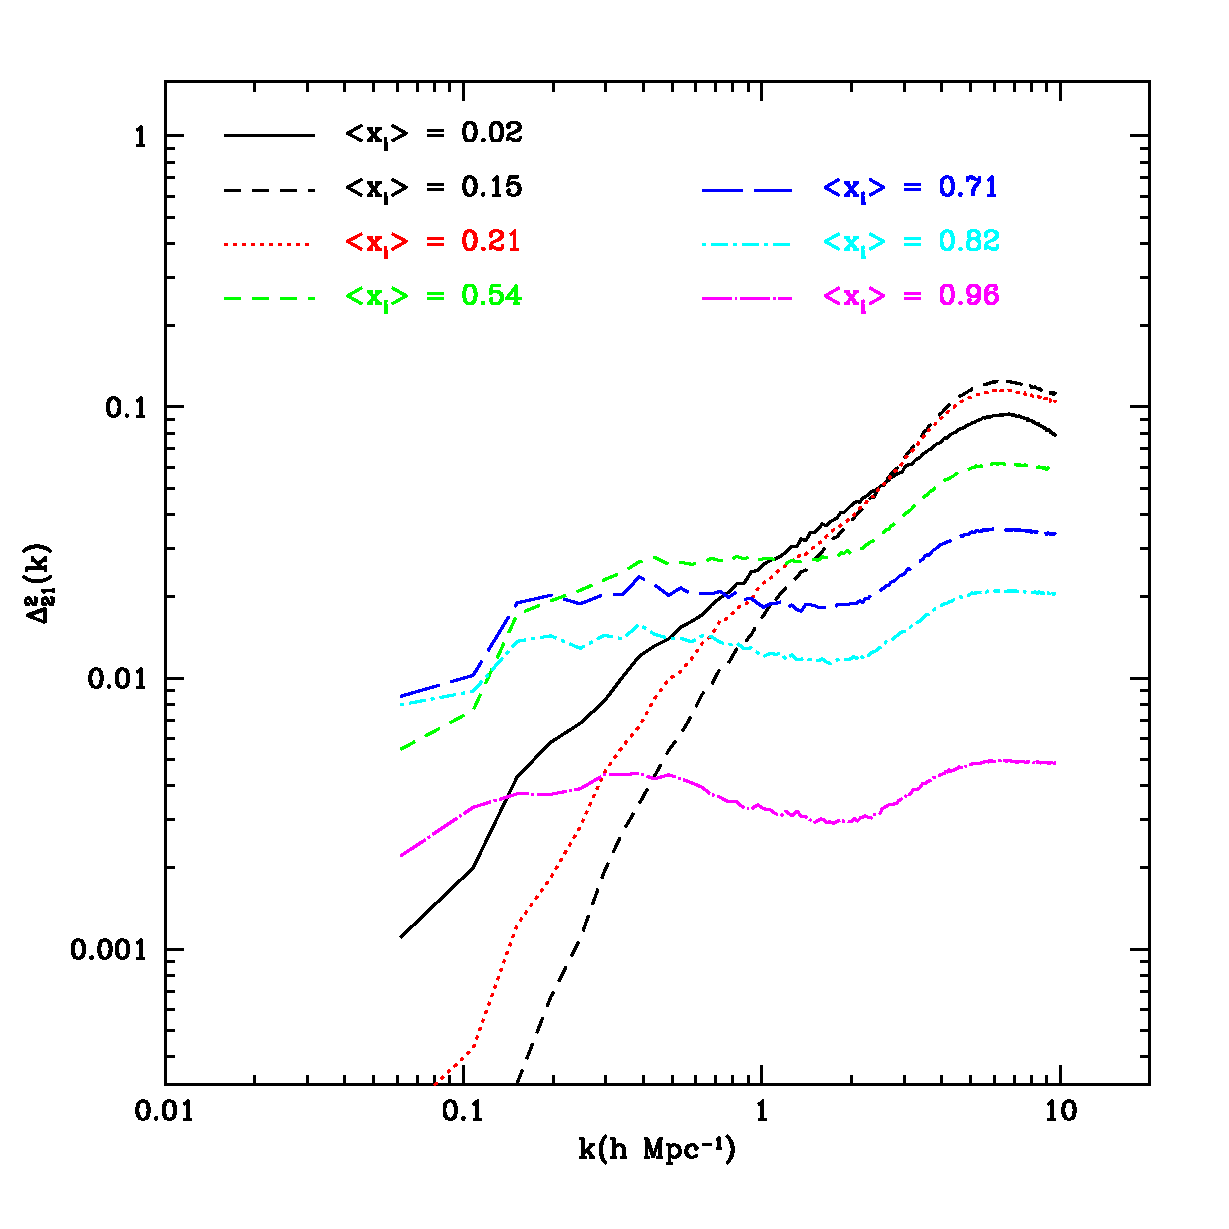
\includegraphics[width=7cm]{LidzPSEvolution.eps}
  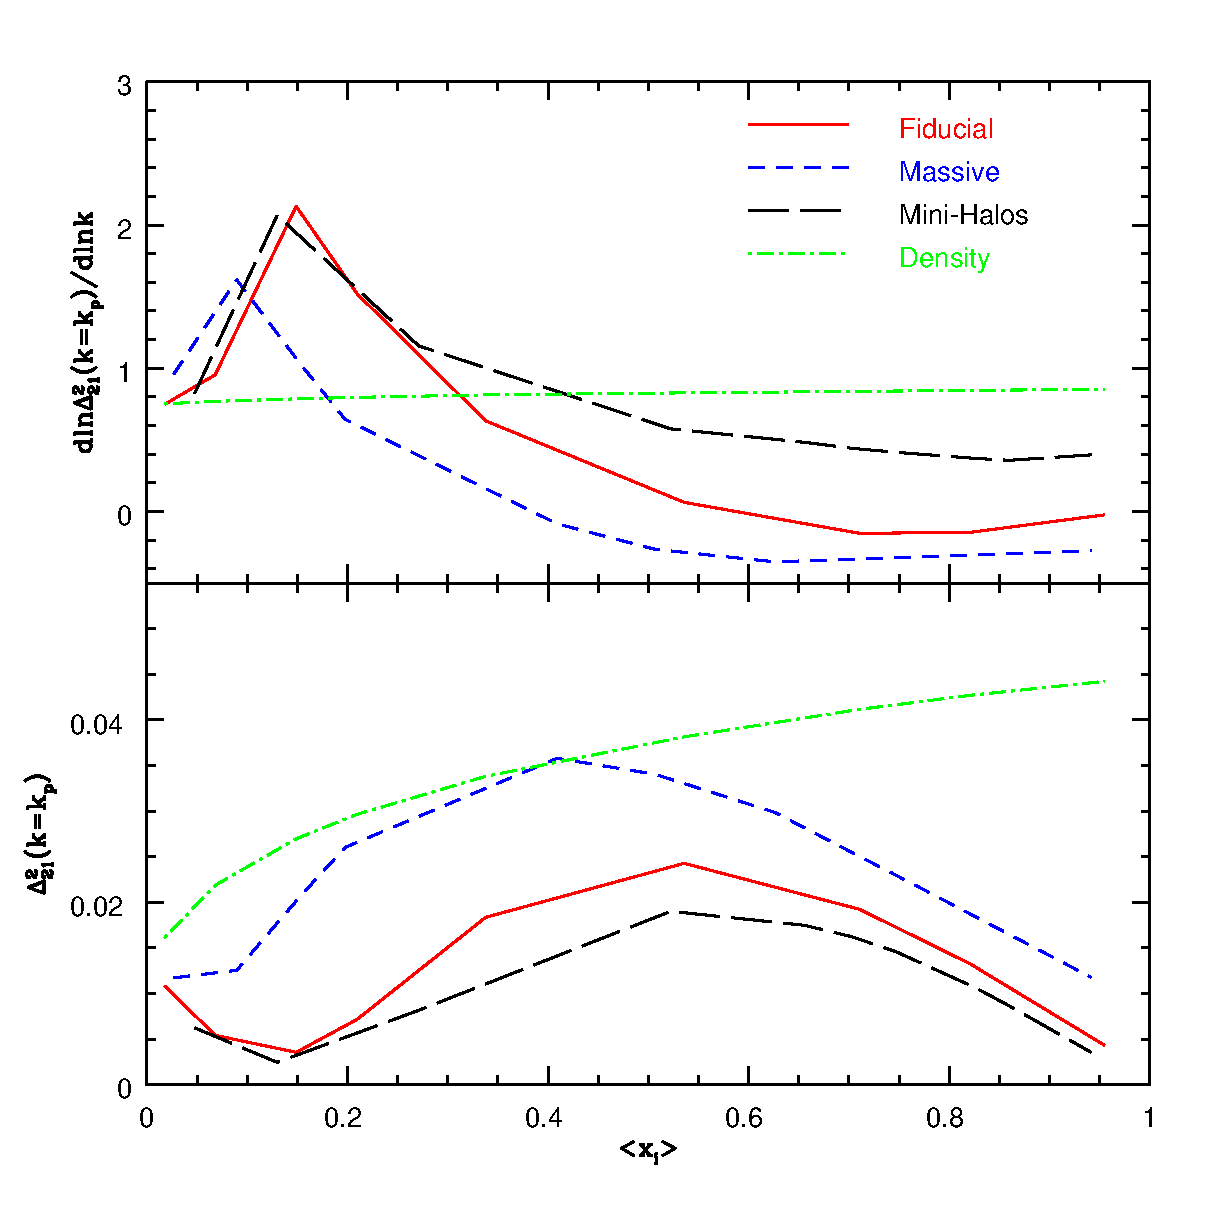
\includegraphics[width=7cm]{LidzSlopeAndAmpEvolution.eps}
  \caption{The left panel shows the evolution of the power spectrum during reionization for the fiducial reionization model in \cite{Lidz2008}. We can see that, as reionization progresses, the slope of the power spectrum in the $k$-mode range accessible to interferometers ($0.1\ h/\text{Mpc} \leq k \leq 1\ h/\text{Mpc}$) declines. The \textit{amplitude} of this part of the power spectrum peaks around $\axhi = 0.5$. The right-hand panel shows the evolution of the power spectrum slope (top) and magnitude (bottom) during reionization for a few different reionization models. This demonstrates that the general power-spectrum evolution described is generic to many reionization models. Both figures are taken from \cite{Lidz2008}.}
  \label{fig:todo}
\end{figure}


Constraints have already been placed on the nature of the EoR using this approach by, for example, the PAPER collaboration. In \cite{ali2015paper} and \cite{pober2015paper}, upper limits on the amplitude of the 21-cm power spectrum at $z = 8.4$ are converted to constraints on the IGM properties. Specifically, we see in Eq. \ref{eq:dTb} that, if $T_{\text{S}} \ll T_{\text{CMB}}$, then the amplitude of the 21-cm signal can become arbitrarily large. As we will touch on in \S \ref{sec:Global21cm}, for redshifts relevant to reionization, the spin temperature is tied to the gas temperature. As such, upper limits on the 21-cm power spectrum amplitude can be converted to lower limits on the spin temperature and therefore also lower limits on the gas temperature. These authors use the upper limits to rule out a very cold reionization scenario. 


Measurements of the 21-cm power spectrum and its evolution are powerful probes of the Epoch of Reionization, but they are inherently indirect. Making detailed maps of the 21-cm radiation field would be much more direct, but will likely be out of reach for first and second generation experiments. However, the presence of an intermediate range in $k$ space which remains relatively un-spoiled by noise could provide us with the ability to make \textit{crude} maps of the 21-cm field and/or directly image individual large ionized regions. Direct observations of individual ionized regions would provide unambiguous evidence that reionization is ongoing and could also provide hints as to the sources of the ionizing photons and the volume-averaged neutral fraction. Such proposed approaches generally attempt to reconstruct the underlying signal by downweighting the $k$ modes of the observed signal which are expected to be dominated by noise. While these techniques are out of reach for first-generation experiments like PAPER, they may very well be suitable for successor experiments, such as HERA. We develop some of these filtering approaches in \S \ref{sec:Bubble} and explore their utility for a variety of plausible experiments.


\clearpage 
\subsubsection{Brief Description of 21-cm Interferometric Experiments}\label{sec:21cmExperiments}


In this section, we provide a brief description of the aforementioned interferometers aimed at detecting the 21-cm signal from the Epoch of Reionization. Much of the descriptions will closely follow information on their respective websites, which are also provided.


The Giant Metrewave Radio Telescope (GMRT\footnote{{\tt http://gmrt.ncra.tifr.res.in/}}) is a collection of 30 very large steerable antennae with a diameter of 45m and is located 80km north of Pune, India. Approximately half of the antennae are configured in a dense central core, with the remaining antennae forming a very extended ``Y'' shape, with the largest baseline being 25km. This multi-purpose experiment has been operating since 1995 and is interested in investigating 21-cm emission from the formation of the first galaxies and reionization, learning about pulsars and neutron stars, and studying properties of the Milky Way, among many other topics. As such, the configuration is not optimized for studying the 21-cm emission from the EoR. A picture of a few of the antennae are shown in Figure \ref{fig:GMRT}.

\begin{figure}[h]
  \centering
  \includegraphics[width=12cm]{GMRT.eps}
  \caption{{\tt http://www.mso.anu.edu.au}}
  \label{fig:GMRT}
\end{figure}


The Donald C. Backer Precision Array to Probe the Epoch of Reionization (PAPER) is a radio interferometer built to detect the power spectrum from 21-cm emission during the EoR. The primary science array is located in the Karoo desert of the Northern Cape in South Africa. The experiment initially deployed 16 antennae in 2009 with the intention of increasing the number of array elements with time. Their most recent constraints (\citealt{pober2015paper}) on the EoR were made using a 64-element configuration, which is currently being expanded to 128 elements. Some of the elements of the array are shown in Figure \ref{fig:PAPER}, which demonstrates one of the the highly-redundant configurations, with many baselines observing the same $k$-mode, optimized for power-spectra measurements.

\begin{figure}[h]
  \centering
  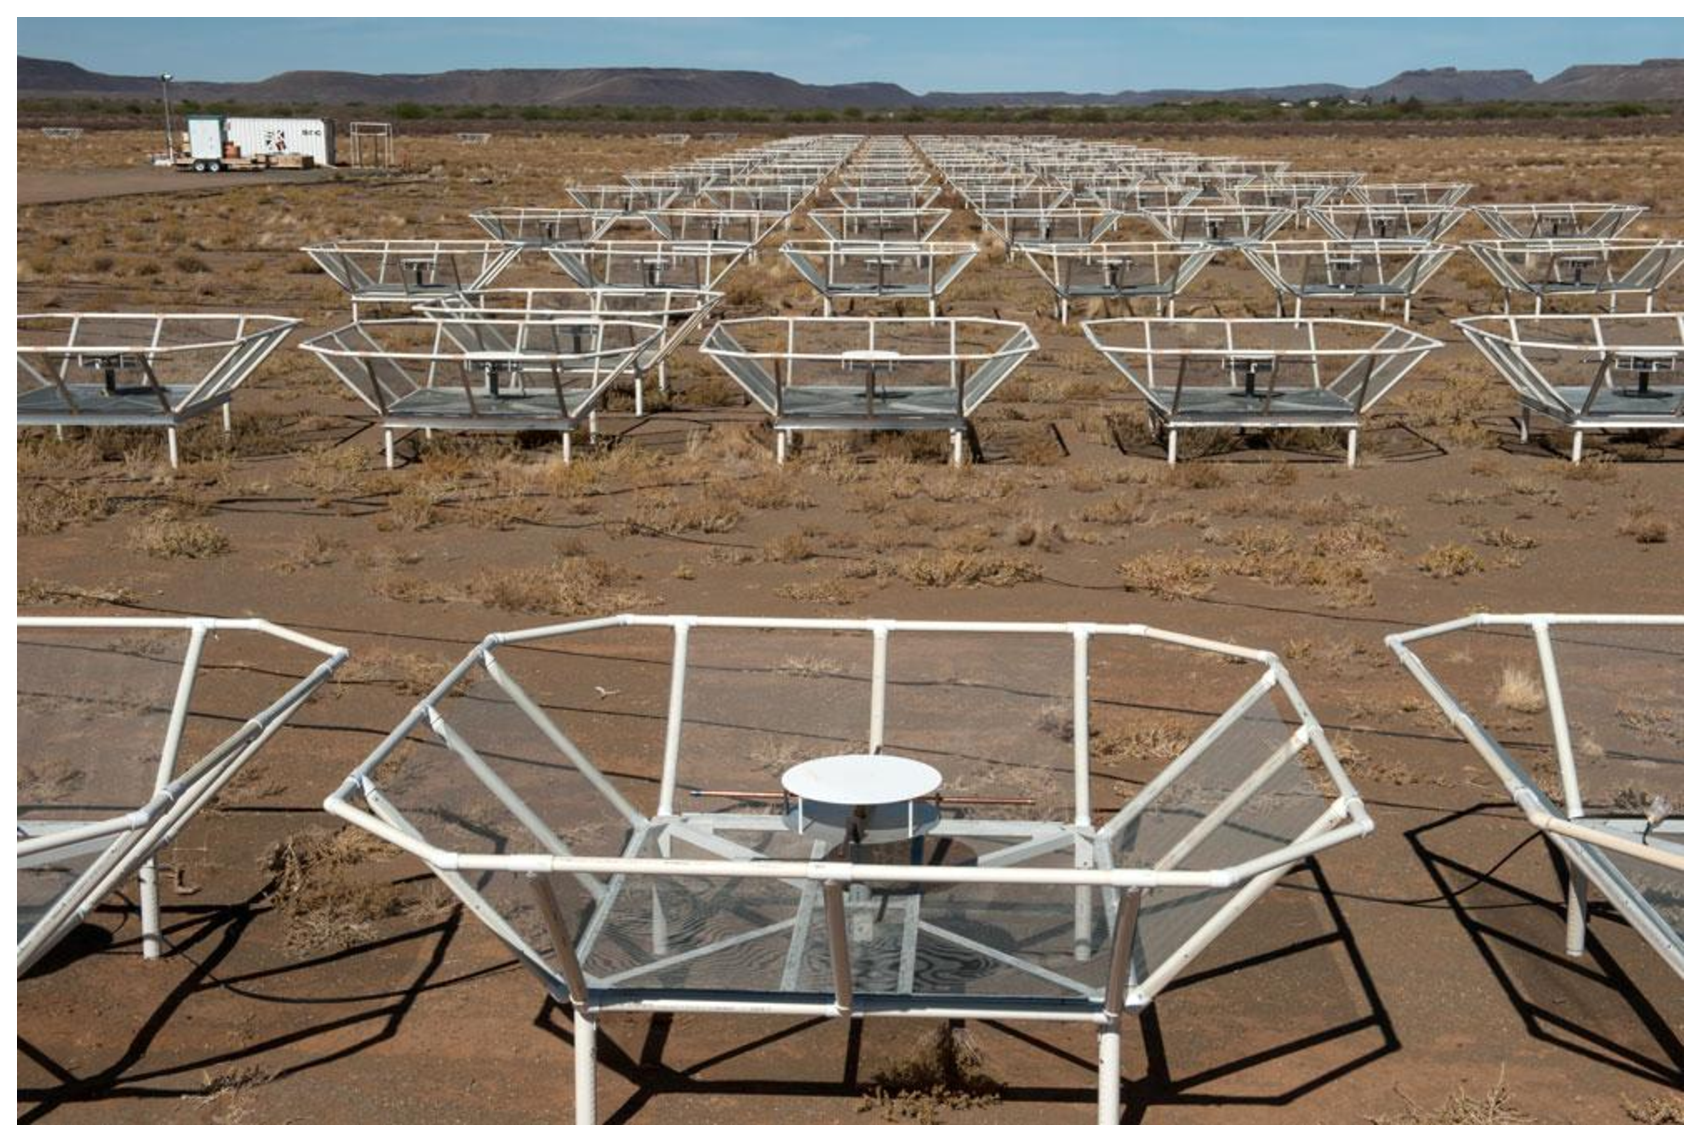
\includegraphics[width=10cm]{PAPER.eps}
  \caption{Picture from {\tt http://discovermagazine.com}}
  \label{fig:PAPER}
\end{figure}


The Murchison Widefield Array (MWA\footnote{{\tt http://www.mwatelescope.org/}}) is a radio interferometer located in the Shire of Murchison in Western Australia. This is a multi-purpose experiment aimed at investigating the EoR, galactic science, transient sources, and space weather. It is composed of 128 antenna tiles, which are each composed of 16 dipole antennae. The majority (112) of the tiles are located within a 1.5km region, with the remaining tiles at larger separations in order to facilitate calibration and to pursue other science goals. The MWA began science observations in 2013. An image of some of the antenna tiles which compose the central core is shown in Figure \ref{fig:MWA}. The array configuration shows much less redundancy compared with PAPER, with tiles placed seemingly-randomly in a configuration more favorable for imaging. The MWA, together with PAPER, is a pathfinder for HERA and is also referred to as HERA Phase I. 

\begin{figure}[h]
  \centering
  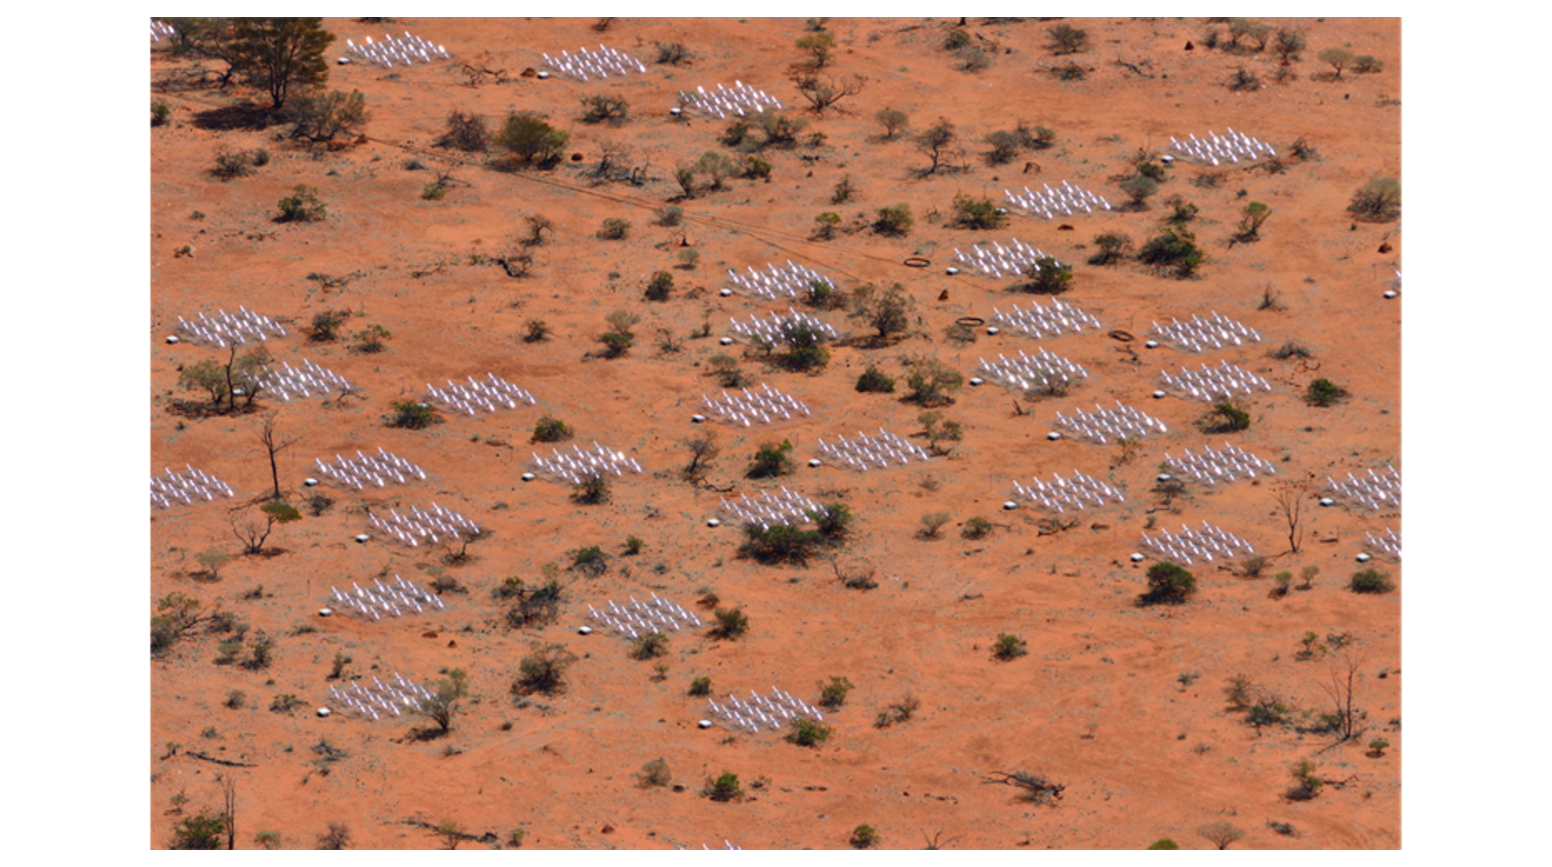
\includegraphics[width=10cm]{MWA.eps}
  \caption{Image taken from {\tt http://www.mwatelescope.org/multimedia} }
  \label{fig:MWA}
\end{figure}


The Hydrogen Epoch of Reionization Array (HERA\footnote{{\tt www.reionization.org}} is an array in preparation which will use understanding gained from both PAPER and MWA in order to make statistical detections and images of the Epoch of Reionization. A potential layout of the HERA experiment is shown in Figure \ref{fig:HERA}, displaying a hexagonal arrangement of 547 elements, each with a 14-meter diameter. As such, this represents an order of magnitude increase in collecting area compared to first-generation experiments.

\begin{figure}[h]
  \centering
  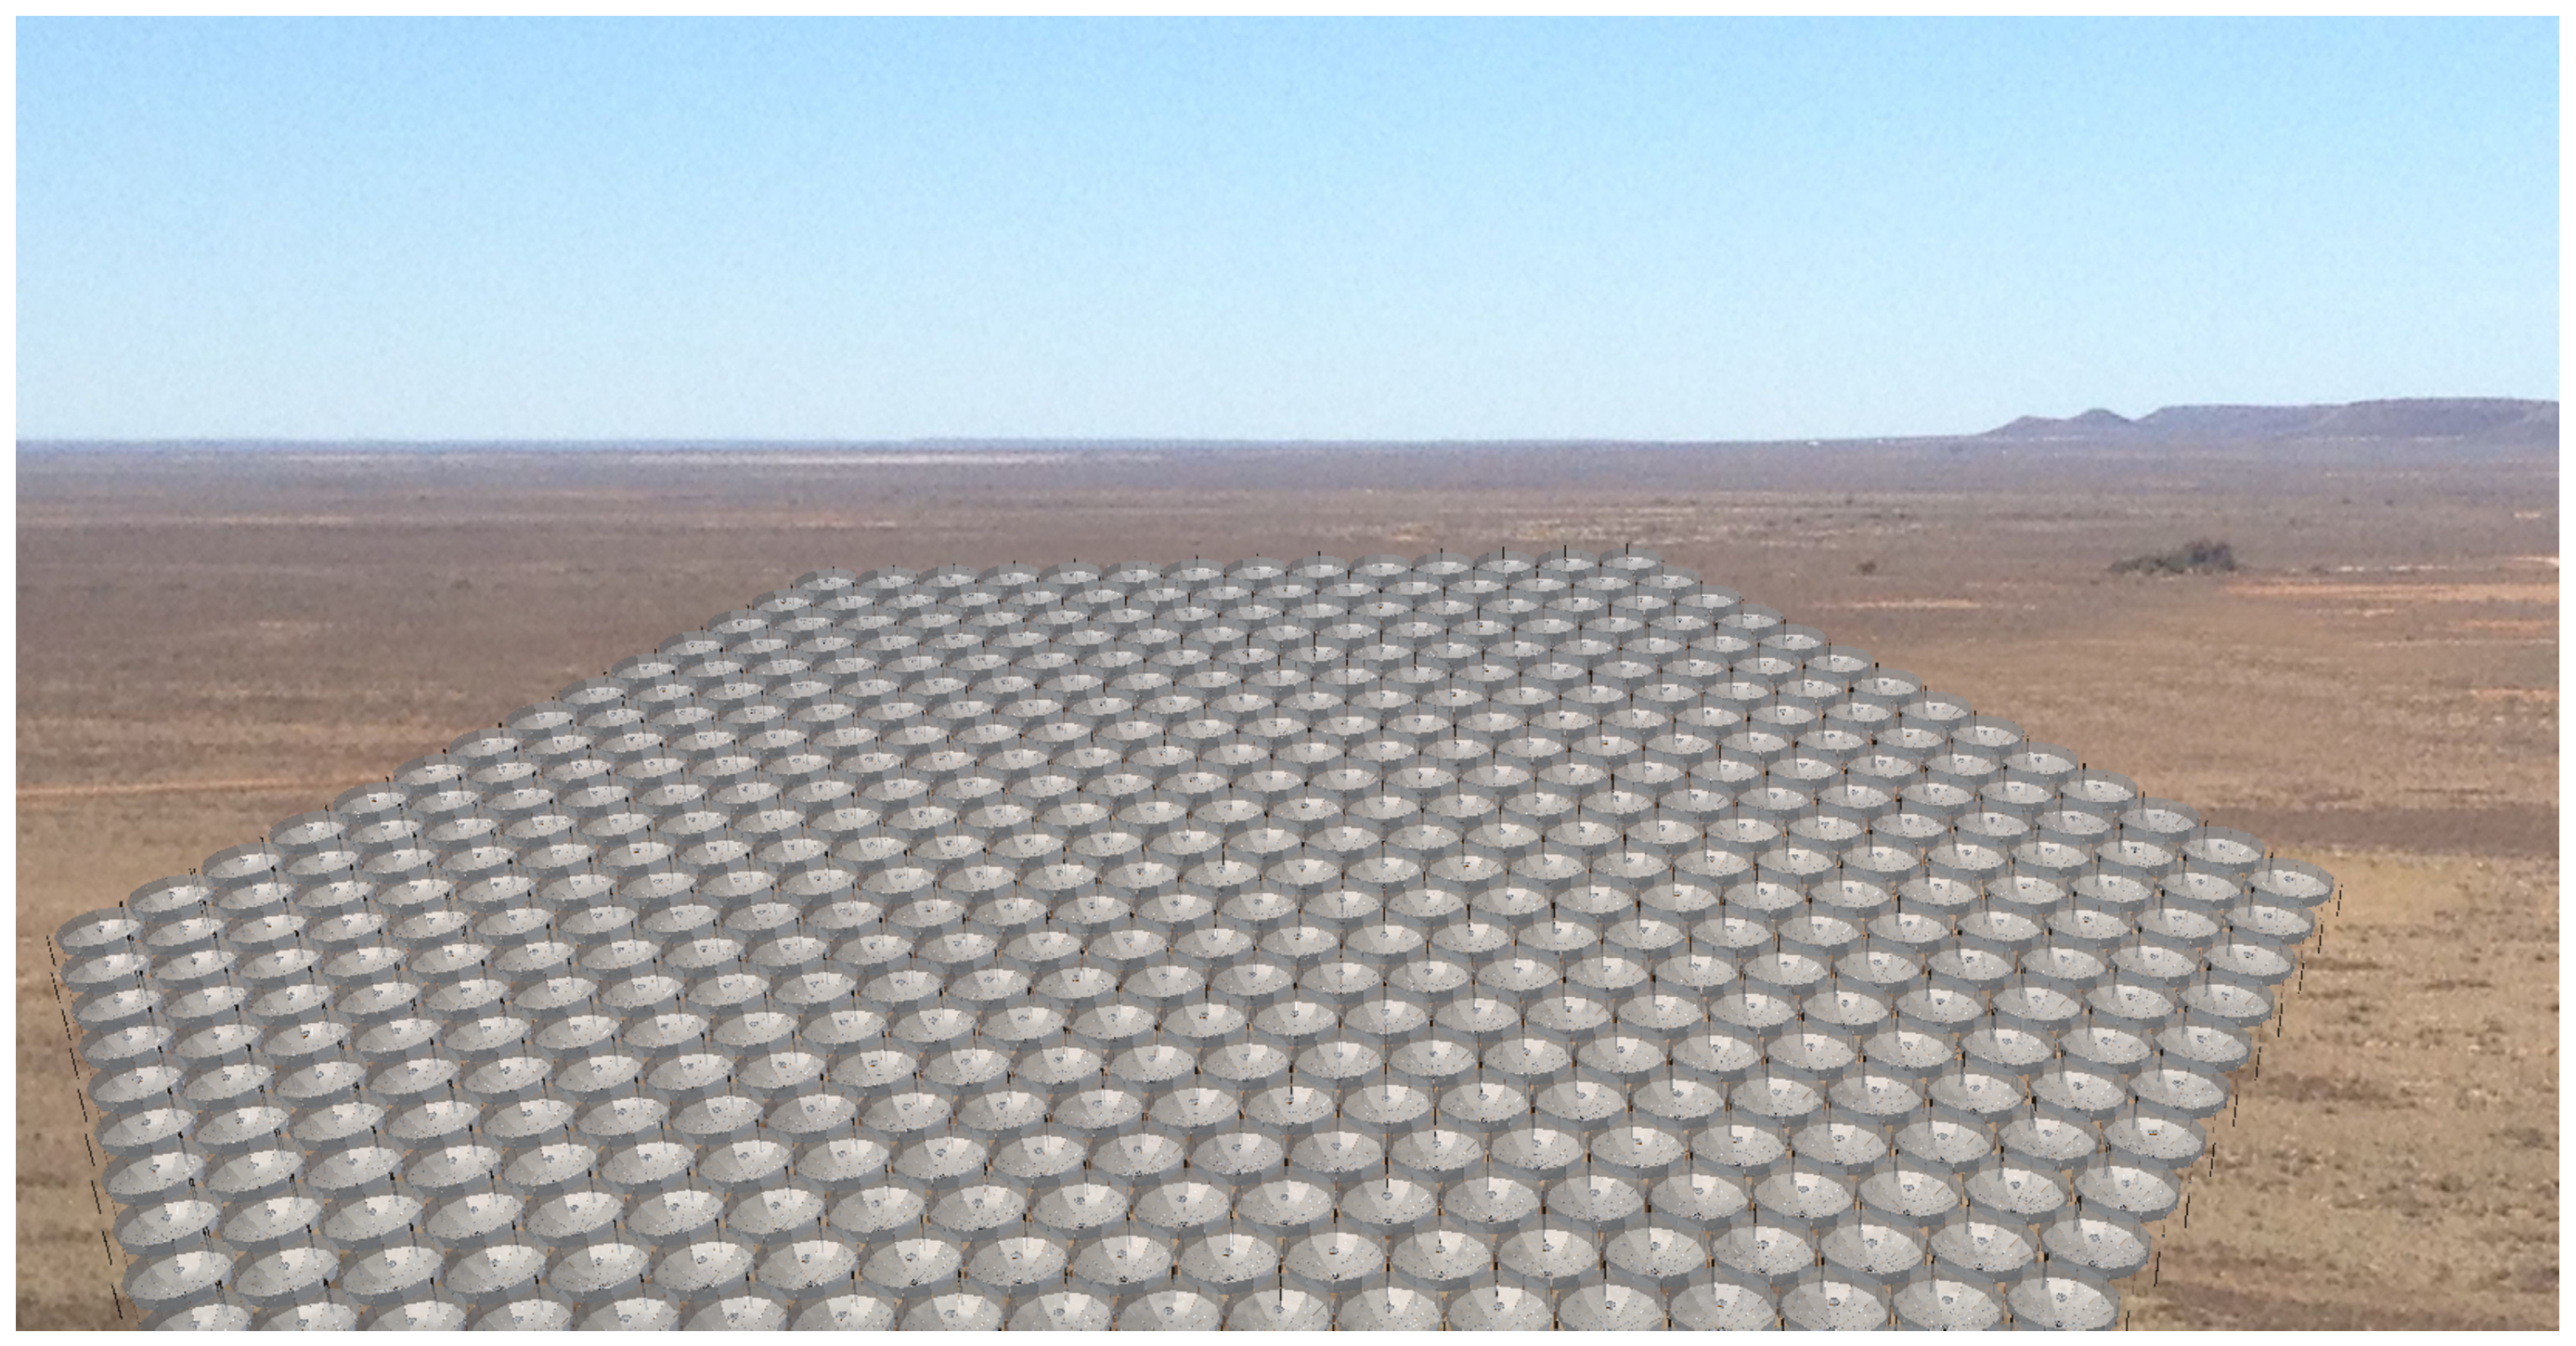
\includegraphics[width=10cm]{HERA.eps}
  \caption{Image taken from {\tt www.reionization.org}.}
  \label{fig:HERA}
\end{figure}

The Low-Frequency Array (LOFAR\footnote{{\tt www.lofar.org}}) is another currently-operational multi-purpose interferometer taking strides toward making a statistical detection of the EoR. In addition to the EoR, the array is also aimed at making deep extragalactic surveys, studying transit radio phenomena, high energy cosmic rays, cosmic magnetism and space weather.\footnote{{\tt http://en.wikipedia.org/wiki/LOFAR\# Key\_projects}} The core of the array is located in the Netherlands but stations of the array are also located in Germany, Great Britain, France, and Sweden. The instrument began observations in late 2012. An image of the central antenna stations is shown in Figure \ref{fig:LOFAR}. Compared to the other arrays discussed thus far, we see LOFAR has larger individual tiles, in a non-redundant configuration, with a significantly larger minimum separation. As such, it will be less sensitive to small $k$-modes, according to Eq. \ref{eq:modes}. Together with the MWA, LOFAR is a pathfinder experiment for the Square Kilometer Array.


\begin{figure}[h]
  \centering
  \includegraphics[width=8cm]{LOFAR.eps}
  \caption{Image taken from {\tt www. astron.nl}.}
  \label{fig:LOFAR}
\end{figure}


Lastly, the Square Kilometer Array (SKA\footnote{{\tt https://www.skatelescope.org/}}) is another later-generation interferometer. Construction is currently expected to begin in 2018, with a planned first light of 2020. The antenna stations will be located in South Africa and Australia. It is another multi-purpose experiment, but the reionization component of the array is expected to be composed of 90 elements, each with a diameter of 100m and is planned to be in Australia. It will make observations of the frequency interval $\text{50MHz} \leq \nu \leq 350\text{MHz}$, corresponding to $3 \leq z \lesssim 30$, in principal allowing for observations prior to the Epoch of Reionization. An artist's impression of what the low-frequency reionization-focused component of the experiment might look like is shown in Figure \ref{fig:SKA}.

\begin{figure}[h]
  \centering
  \includegraphics[width=8cm]{SKA.eps}
  \caption{An aritist's impression of what the reionization-focused element of the SKA might look like. "SKA sparse array big" by SKA Project Development Office and Swinburne Astronomy Productions - Swinburne Astronomy Productions for SKA Project Development Office. Licensed under CC BY-SA 3.0 via Wikimedia Commons.}
  \label{fig:todo}
\end{figure}



\clearpage
\subsubsection{The Global 21-cm Signal}\label{sec:Global21cm}

An alternative method of extracting information from the 21-cm line is to use the \textit{sky-averaged} 21-cm signal. In the previous section, we discussed the difficulties faced in obtaining the necessary resolution to map out fluctuations in the 21-cm radiation field. However, Equation \ref{eq:dTb} is rich with astrophysical information on its own without even considering spatial fluctuations. Therefore, natural questions to ask would be if it is easier to simply measure the average signal rather than map the fluctuations and what astrophysical information can be obtained in that way? For convenience, the brightness temperature contrast for the 21-cm signal from \S \ref{sec:21cmPhysics} is:


\begin{align}
\delta T_{b} &\approx 24 \text{mK}\cdot x_{\text{HI}}(1+\delta)\left(\frac{1+z}{7}\right)^{1/2}\left[ 1 - \dfrac{T_{\text{CMB}}}{T_{\text{S}}} \right] \left[ \dfrac{H(z)/(1+z)}{\dd v_{\parallel}/ \dd r_{\parallel}} \right].
\end{align}


As mentioned earlier, for the end of reionization, it is true that $T_{\text{S}} \gg T_{\text{CMB}}$ such that the dependence on spin temperature drops out. The result is that the amplitude of a sky-averaged signal is most sensitive to the neutral faction, with ionized regions emitting no 21-cm signal and neutral regions emitting 21-cm radiation with brightness temperature of tens of mK.  Thus, one could imagine plotting the sky-averaged 21-cm signal throughout the EoR against redshift and observing a shrinking signal toward lower redshifts coinciding with a larger fraction of the volume of the Universe being ionized.


However, the utility of the global 21-cm signal is not limited to the Epoch of Reionization. Specifically, prior to reionization, $\axhi$ will be fixed at 1 and the spin temperature is expected to drop to the point where $1 - T_{\text{CMB}}/T_{\text{S}} \not\approx 1$. Therefore, the strength of the 21-cm radiation field will be tied to the spin temperature instead of the neutral fraction. Furthermore, the 21-cm signal will only be observable if $T_{\text{S}} \neq T_{\text{CMB}}$ and will appear in emission if $T_{\text{S}} > T_{\text{CMB}}$ and will appear in absorption otherwise. This is interesting because the spin temperature itself depends on several astrophysical processes. A very high-level description of this is shown in Figure \ref{fig:TsEvolution}.\footnote{This figure and much of the following discussion is taken from notes from Adam Lidz's ``Topics in Cosmology'' class, taught in the Fall of 2011.} The precise evolution of the spin temperature is not well known, but a reasonable approximate description could be as follows:

\begin{enumerate}
\item [] \underline{$z > 150$:} Collisions within the gas are frequent enough to fix the spin temperature to the gas temperature, $T_{\text{S}} = T_{\text{K}}$. However, the gas temperature is equal to the CMB temperature, so the 21-cm signal is \textit{unobservable}.
\item [] \underline{$30 < z < 150$:} Collisions are efficient at coupling the gas temperature to the spin temperature. Furthermore, the gas cools to below the CMB temperature, making the 21-cm signal \textit{obervable}. The physics during this time, prior to the formation of the first galaxies, is relatively simple and so this portion of the signal is expected to be well-understood already. 
\item [] \underline{$20 < z < 30$:} The gas density drops enough so that collisions are not efficient at coupling the spin temperature to the gas temperature. As a result, the spin temperature approaches the CMB temperature and the 21-cm signal is \textit{unobservable}. 
\item [] \underline{$15 < z < 20:$} Wouthuysen field effect re-couples the spin temperature to the gas temperature, which is still below the CMB temperature. This renders the 21-cm signal \textit{observable in absorption}. 
\item [] \underline{$ z < 15:$} The first X-ray sources form and heat the gas well above the CMB temperature. As a result, the 21-cm signal becomes \textit{observable in emission}.
\item [] \underline{$ z \lesssim 5.5:$} The completion of reionization effectively eliminates the 21-cm signal from the IGM all together. The 21-cm signal is still observable in pockets of neutral gas surrounding galaxies. 
\end{enumerate}


\begin{figure}[!p]
  \centering
  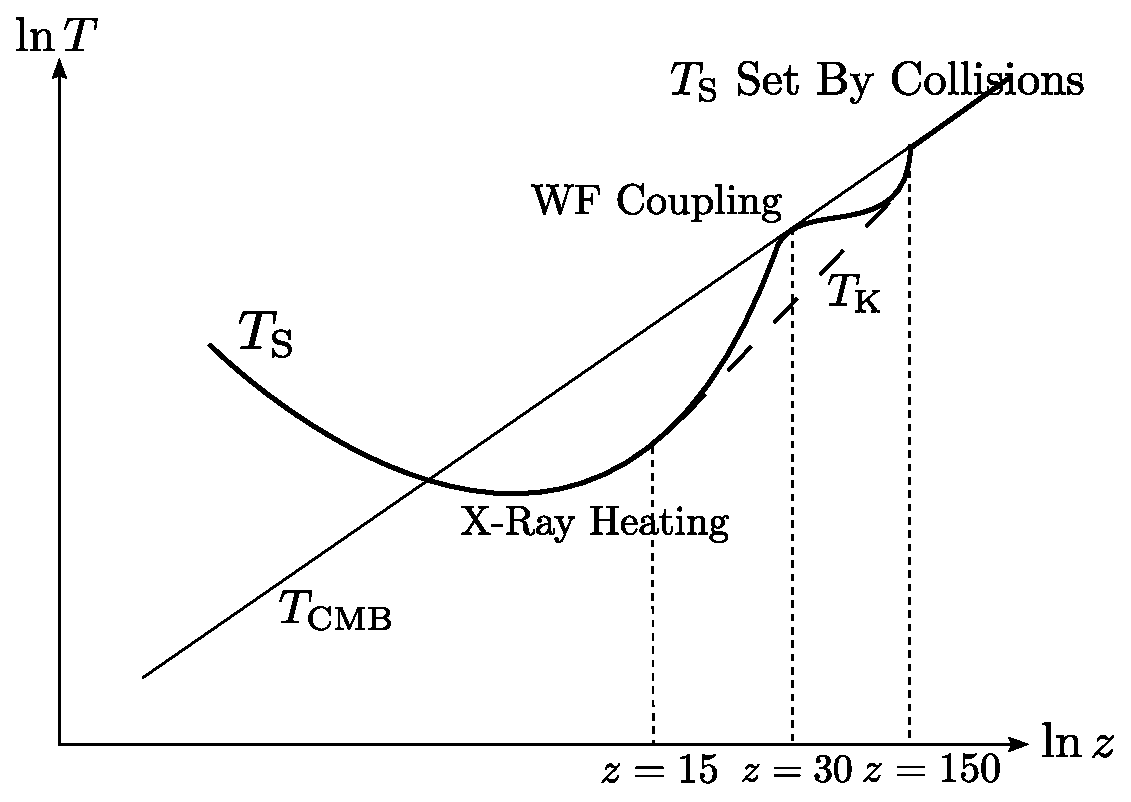
\includegraphics[width=12cm]{TsEvolution.eps}
  \caption{Schematic representation of a plausible $T_{\text{S}}$ signal including a few landmarks. This is adapted from notes taken in the course ``Topics in Cosmology''.}
  \label{fig:TsEvolution}
\end{figure}


While the expected globally-averaged 21-cm signal during $z > 30$ (and $z < 5$) is well-understood, much of the rest of the signal is very uncertain. Therefore, we could imagine measuring $\delta \bar{T}_{b}(z)$ in order to constrain some of the underlying astrophysics during this time period. However, as we discussed in \S \ref{sec:21cmFluctuations}, the foreground noise is several orders of magnitude larger than the 21-cm signal during the EoR and varies \textit{smoothly} with frequency. When considering 21cm fluctuations, we were saved by the fact that the signal fluctuated rapidly along any individual line of sight. However, when considering the \textit{average} 21-cm signal, fluctuations should be very smooth along the line of sight. 


Specifically, from the end of reionization to the beginning, the global 21-cm signal should increase from $\delta \bar{T}_{b} = 0$ to $\delta \bar{T}_{b} \gtrsim 30$mK. As such, a drawn-out and extended reionization scenario will be relatively difficult to detect. However, in the case of a rapid reionization of the Universe, it is conceivable that this evolution could be quite steep. \cite{bowman2010lower} measured the global 21-cm signal for three months in the frequency range $100\text{MHz} \leq \nu \leq 200\text{MHz}$, corresponding to $6 < z < 13$, and found the evolution in the signal to be sufficiently smooth as to constrain $\Delta z_{r} > 0.06$ with 95\% confidence. 


Another experiment which has gained some attention in this sector is the Dark Ages Radio Explorer (DARE, \citealt{burns2012probing}) which aims to measure the turning points and slope of the 21-cm signal (shown in Figure \ref{fig:TsEvolution}) over the redshift range $11 \leq z \leq 35$ in order to constrain the formation of the first stars, galaxies, accreting black holes along with the amount subsequent X-ray heating, and constrain the beginning of the EoR.\footnote{This information about DARE was obtained from {\tt http://lunar.colorado.edu/}} This will be done by placing a 21-cm antenna in lunar orbit. It is interesting to note that, even at this seemingly-ideal observation location, much effort will be needed to isolate nuisance contributions to the 21-cm signal, such as those from foreground emission from our own galaxy, the Sun, thermal emission from the Moon, and reflected galactic foregrounds off of the surface of the Moon (\citealt{harker2012mcmc}).

\clearpage
\subsection{The Cosmic Microwave Background}\label{sec:CMB}


The Cosmic Microwave Background (CMB) is the earliest accessible picture we have of the Universe. It is composed of photons which have travelled, largely uninterrupted, from when the Universe was $\sim380,000$ years old\footnote{This is $\sim3\times 10^{-3}\%$ of its current age. If the Universe were an 80-year-old human, then the CMB would provide a picture of him/her when they were less than a day old.} to us today. Before this time, the Universe was hot enough that collisions between its constituent parts prevented the formation of neutral atoms (mostly hydrogen and helium). As a result, photons had an extremely short mean free path between collisions with free electrons. This makes this period of time completely opaque and impenetrable by observations. However, at $\sim380,000$ years, the Universe cooled to the point where neutral hydrogen could form (neutral helium having formed slightly earlier) and capture almost all of the remaining free electrons. Without a substantial number of free electrons, the mean free path of photons increased to the point where they could reach us today. Because of this, this CMB is also referred to as the ``surface of last-scattering''.


Therefore, the CMB is essentially a picture of the Universe at the time when photons decoupled from matter. As a result, it provides us with a picture of the matter distribution at this time and its value to cosmology cannot be overstated. While this is wonderful, in this thesis we are interested in the evolution of the Universe when it was $\sim500$ million years old, not $\sim380,000$, so how can the CMB help us? 


Well, similarly to how bright light from distant quasars/GRBs can give us information on the intervening gas, light from the CMB can do the same. While $\gtrsim90\%$ of photons will travel from the surface of last scattering to us without interacting, the other $\lesssim10\%$ of the photons will scatter off of free electrons that have been released as a result of reionization. Therefore, an interesting question is if this level of interaction can create an observable imprint in the CMB itself. In this section, we briefly discuss two such methods for searching for these imprints and their progress toward constraining the EoR.


\subsubsection{Thompson Scattering Optical Depth, $\tau_{e}$}


The first observable that we discuss is the CMB optical depth to Thompson scattering. As mentioned earlier, after the time of the surface of last-scattering, the density of free electrons drops low enough to allow photons to travel unimpeded. However, once reionization is underway, free electrons will be introduced into the IGM and will scatter a significant number of the CMB photons. The precise fraction of CMB photons that scatter in this way depends on the integrated electron density along the line of sight to the CMB. This is sensitive to the timing of reionization since CMB photons will have the opportunity to scatter off of electrons over a larger path length if reionization happens earlier. The percentage of CMB photons which scatter in this way is quantified through the Thompson scattering optical depth, $\tau_{e}$, where

\begin{align}
f_{\text{scattered}} &\approx 1-e^{-\tau_{e}} \approx \tau_{e}
\end{align}

for small $\tau_{e}$. This is related to the density of electrons along the line of sight via\footnote{We have neglected the contribution to $n_e$ from singly-ionized helium in this expression for simplicity.}

\begin{align}
\tau_{e} &= \int \dfrac{\dd z\ c}{(1+z)H(z)}n_{e}(z)\sigma_{\text{Thom}}\\
&\approx \int \dfrac{\dd z\ c}{(1+z)H(z)} \bar{n}_{\text{H}}(z)(1 - \langle x_{\text{HI}}(z)\rangle) \sigma_{\text{Thom}} \label{eq:taue}
\end{align}

where 

\begin{align}
\sigma_{\text{Thom}} &= \dfrac{8\pi}{3}\left(\dfrac{\alpha \hbar}{m_ec}\right)^2 \approx 6.65\times 10^{-25}\cm^{2}
\end{align}

is the frequency-independent cross section for Thompson scattering, $\alpha \approx 1/137$ is the fine structure constant\gloss{$\alpha$}{Fine structure constant, $\alpha \approx 1/137$, related to the strength of electromagnetic interactions.}, $\hbar$ is the reduced Planck's constant\gloss{$\hbar$}{Reduced Planck's constant, $\hbar = h/2\pi$, the quantum of angular momentum.}, and $m_e$ is the mass of the electron. The integral is carried out from $z = 0$ to the surface of last scattering ($z \approx 1080$). Thus, we see that a measurement of the optical depth for CMB photons Thompson scattering off of electrons released during reionization would be an integral constraint on $\langle x_{\text{HI}}(z)\rangle$. Typically, such measurements of $\tau_{e}$ are converted into a redshift of ``instantaneous reionization'', $z_{r}$, by performing the integral assuming $\axhi = 0$ for $z < z_{r}$ and $\axhi = 1$ for $z > z_r$ and finding which value of $z_{r}$ produces the same $\tau_{e}$. The model of an instantaneous reionization is not to be taken seriously, but this quantity provides a rough upper bound on the half-point of reionization.\footnote{It is not an exact half point because free electrons at higher $z$ will have a larger contribution to the optical depth due to the increased density of the Universe at that time.} 


In order to measure $\tau_{e}$ we can take advantage of the tendency for photons to have their polarization altered when they undergo Thompson scattering. Specifically, photons propagate such that their E-field and B-field oscillate in directions perpendicular to their direction of travel. When a photon gets scattered into our line of sight, it maintains its original polarization in the plane perpendicular to the line of sight. As such, the net polarization from a point on the sky depends on the anisotropies in the radiation field present in that point of the sky. This is illustrated in a diagram by Wayne Hu in Figure \ref{fig:tauEPolarization}. This shows that, due to the intensity of radiation incident on an electron from the left and right being greater than the intensity of radiation incident on the electron from above and below, a net \textit{vertical} polarization signal is generated from repeated Thompson scatterings off of this electron. 


The electrons sourcing the polarization signal will see radiation from the quadrupole isotropy on scales of the horizon size at the time of the scattering. Therefore, fluctuations in the observed polarization signal will occur on spatial scales equal to the horizon size at the time of reionization. This allows measurements of the polarization power spectrum to be translated into a measurement of $\tau_{e}$.   Current measurements from \cite{planck2015planck} determine $\tau_{e} = 0.066 \pm 0.0121$, which translates to $z_{r} = 8.8^{+1.2}_{-1.1}$. Interestingly enough, this is a substantial shift from the first-year WMAP measurement of $\tau_{e} = 0.166^{+0.076}_{-0.071}$, $z_{r} = 17\pm 4$, and even a substantial shift from the nine-year WMAP results of $\tau_{e} = 0.089\pm 0.014$, $z_{r} = 10.6\pm 1.1$ (	\citealt{Bennett2013}). This contributes to some of the accumulating evidence that reionization may have occurred later (lower $z$) than was originally believed and makes measurement techniques applicable to $z \lesssim 6$ more interesting.

\begin{figure}[!p]
  \centering
  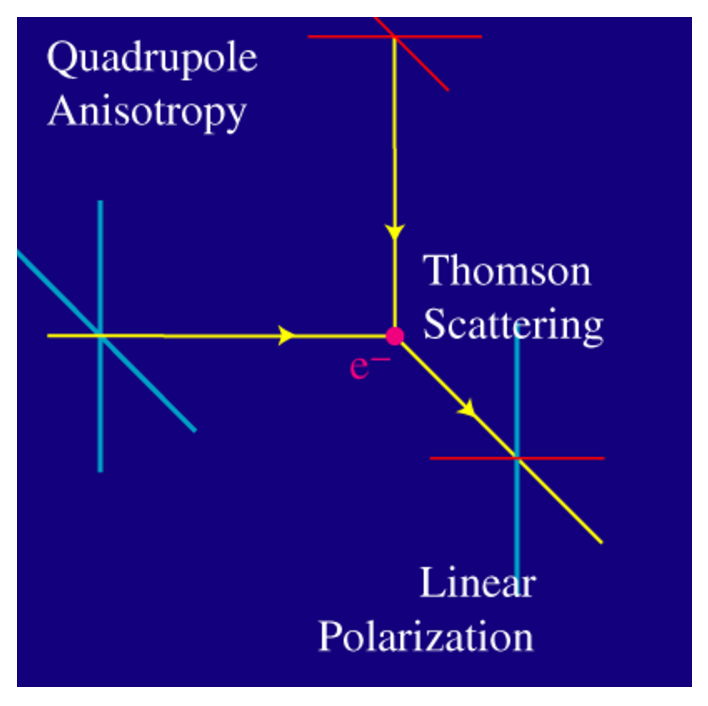
\includegraphics[width=8cm]{tauEPolarization.eps}
  \caption{An illustration (Wayne Hu, {\tt http://background.uchicago.edu/~whu/}) of how a net polarization signal is generated from Thompson scattering due to the presence of a quadrupole anisotropy. The blue cross and red cross show relatively strong and weak incident radiation, respectively, on an electron at the origin. The red/blue cross indicates the average polarization of scattered light and demonstrates that it obtains a net vertical polarization.			}
  \label{fig:tauEPolarization}
\end{figure}




\clearpage
\subsubsection{Kinetic Sunyaev-Zel'dovich Effect}

The second method of utilizing the CMB to constrain reionization that we discuss is the kinetic Sunyaev Zel'dovich effect (kSZ)\gloss{kSZ Effect}{Kinetic Sunyaev Zel'dovich effect. This describes secondary anisotropy in the CMB produced by the bulk velocities of free electrons during and after reionization which impart a Doppler shift on CMB photons.}. This refers to the secondary CMB anisotropies imprinted on the CMB by the bulk velocities of clouds of free electrons which impart a Doppler shift on the CMB photons. 


The kSZ signal is generally broken down into two contributions: the Doppler shift caused by bulk motions of free electrons \textit{after} reionization completes, and the Doppler shift due to the bulk motions of free electrons in ionized bubbles \textit{during} reionization. As such, the former contribution is known as the ``homogeneous'' (or, alternatively, Ostricker-Vishniac [OV]) kSZ signal and the latter is referred to the ``patchy'' kSZ signal. The homogeneous kSZ signal is sourced by density inhomogeneities on relatively linear scales and should be able to be modelled well (\citealt{mesinger2012kinetic}), allowing the isolation of the patchy contribution.


The patchy kSZ signal is actually sensitive to several parameters of reionization. First, unlike with $\tau_{e}$ measurements, the patchy kSZ contribution only arises \textit{during} reionization. Therefore, the magnitude of the signal itself is related to the duration of reionization since, for a longer reionization, CMB photons will have an opportunity to be Doppler shifted by ionized bubbles over a larger path length. Second, since the patchy kSZ signal is sourced by ionized bubbles, it will important at these bubbles' size scales and the strength of the signal will increase with patchier models of reionization. As such, a detection of a \textit{small} kSZ signal could also be indicative of a more homogeneous reionization, possibly with significant contributions from X-rays (\citealt{visbal2012gauging}).

The South Pole Telescope (SPT) attempted a measurement of this effect (\citealt{Zahn2012}) and interpreted the results in terms of a constraint on the duration of reionization, $\Delta z \equiv z_{\axhi=1} - z_{\axhi = 0.2}$. They were not able to make a detection of the effect but were able to place upper bounds on it, suggesting that $\Delta z < 7.9$ at 95\% confidence.\footnote{Technically, this constraint allows for a free parameter describing the level of correlation between the thermal SZ effect and the Cosmic Infrared Background. Without allowing for this free parameter, their constraint is $\Delta z < 4.4$ at 95\% confidence.}

\clearpage
\subsection{\lya\ Emitters}

\lya\ emitters (LAEs)\gloss{LAE}{\lya\ Emitter. These are galaxies which emit a significant fraction of their energy in the \lya\ line. This line is produced when hydrogen atoms within the galaxy recombine after being ionized by the galaxy. Roughly 2/3 of recombinations result in a \lya\ photon.} are galaxies which emit strongly in the \lya\ line. This \lya\ emission results from hydrogen atoms within the galaxy recombining after being ionized by the galaxy's UV radiation. During $\sim2/3$ of hydrogen recombinations, a \lya\ photon will be emitted. Therefore,  enough ionizations will result in a strong \lya\ line being emitted from the galaxy. 


However, whether or not that \lya\ line is observable to us depends on the intervening gas. Specifically, \lya\ photons produced within the galaxy will repeatedly be absorbed and re-emitted by hydrogen in the galaxy's interstellar medium until it reaches the IGM. At this point, if the IGM is ionized the \lya\ photon will escape. However, if the IGM is significantly neutral, then the \lya\ photon will be scattered into a low-surface-brightness halo, rendering the \lya\ line unobservable (\citealt{finlator2012recent}). This provides us with an observable which depends on the ionization state of the IGM! In this section, we briefly discuss two methods of utilizing this behavior in order to constrain $\axhi$.

%at \axhi = 0.5, LAEs residing in HII regions will typically be one of thousands that contribution to ionizing the HII regions. These regions can be \sim 10 Mpc. However, lya photons only need to travel 1 Mpc in order to redshift out of resonance and escape. 

\subsubsection{Clustering of \lya\ Emitters}

One approach for utilizing LAEs to constrain $\axhi$ is to look at their measured clustering. When the IGM is fully-ionized, the \lya\ lines of all observed galaxies should be visible to us. When the Universe is fully-neutral, then all observed galaxies should lack a strong \lya\ emission line. However, when reionization has progressed such that $\axhi \approx 0.5$, the Universe should represent a two-phase medium consisting of large ($\sim 10\mpch$) ionized regions maintained by thousands of galaxies (\citealt{McQuinn:2007dy}), and significantly-neutral regions which are shielded from the ionizing radiation. The \lya\ line from LAEs located within the large ionized regions should remain intact, as the photons will redshift out of \lya\ resonance after travelling only $\sim 1\mpch$ without encountering significantly-neutral hydrogen (\citealt{finlator2012recent}). Therefore, the LAEs observable when the Universe is 50\% ionized should more often reside in these ionized bubbles with many other sources, resulting in their observed distribution being \textit{highly clustered}. Meanwhile, at lower redshift, all LAEs should be observable (with regard to HI attenuation), resulting in a more uniform distribution.

In Figure \ref{fig:McQuinnLAEClustering}, \cite{McQuinn:2007dy} demonstrate this effect. The top row shows the ionization field (black is neutral, white is ionized) at three different neutral fractions: $\axhi = 0.7$ (left), 0.5 (middle), and 0.3 (right). The second row shows the true underlying LAE locations and the bottom row shows the observed LAEs. Since LAEs should only be observable within ionized regions, we see that the sources in the bottom row must coincide with white regions in the top row, resulting in enhanced clustering of the observed sources.

In \cite{Ouchi2010}, the authors analyze 207 LAEs at $z \sim 6-7$ and compare their clustering with those measured at $z = 5.7$. They find no detection of an enhancement in the observed LAE clustering, suggesting that the bulk of reionization occurred at $z > 6.6$. 



\begin{figure}[!p]
  \centering
  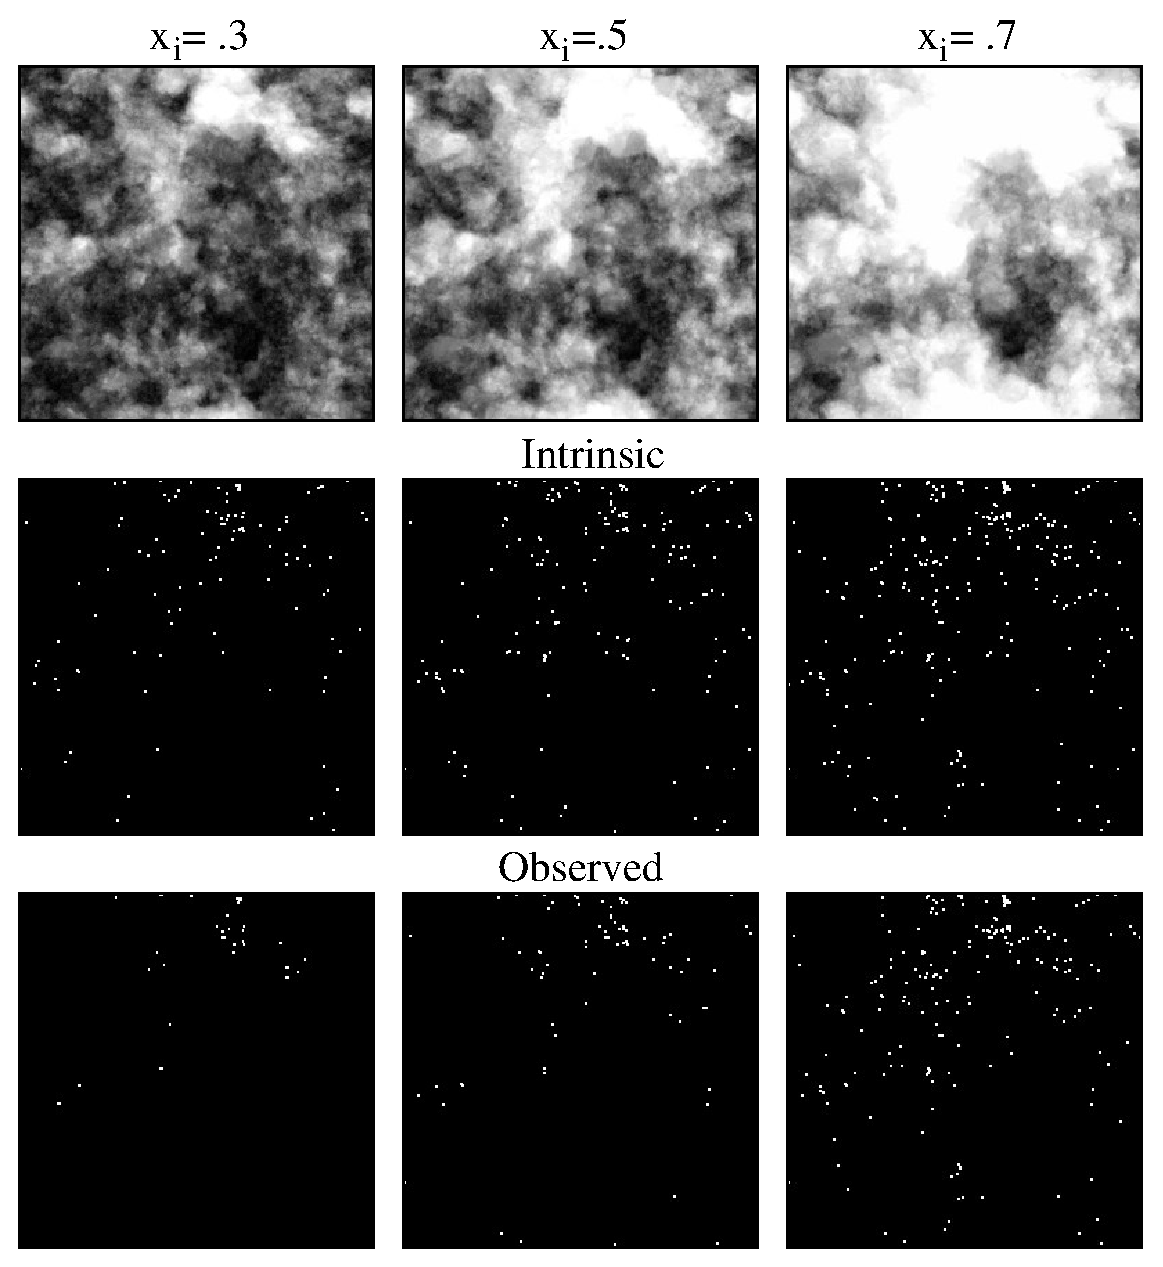
\includegraphics[width=13cm]{McQuinnLAEClusteringLarge.eps}
  \caption{The (simulated) effect of the neutral fraction on the observed clustering of LAEs (taken from \citealt{McQuinn:2007dy}). The top panels show the underlying ionization fields, the middle row shows the true location of LAEs in the simulation, and the bottom panel shows the detectable LAEs in the simulation. This shows that, LAEs which occupy the same ionized bubble will be observable, resulting in a less homogeneous field of observable LAEs. Each panel is 94 Mpc across. }
  \label{fig:McQuinnLAEClustering}
\end{figure}

\clearpage
\subsubsection{\lya\ Emitter Fraction}

As discussed in the previous section, as we move further back in redshift and deep into the reionization process, galaxies that intrinsically have a significant \lya\ line will not be observed as having one. However, the galaxies themselves will still be detectable via the drop-out technique, which searches for sources with significant emission at energies below the Lyman limit\gloss{Lyman Limit}{This refers to the most energetic transition in the Lyman series corresponding to ionizing a hydrogen atom in the ground state. This has wavelength $\lambda = 912$\AA and $E_{\gamma} = 13.6$eV.} and significantly less emission at greater energies. 


As we move further back in redshift, we expect the fraction of detected galaxies which \textit{would} have a \lya\ line but do not, due to a significantly-neutral IGM, will increase. While we do not have access to this exact measurement of this fraction, we \textit{can} measure the \textit{overall} fraction of detected galaxies which exhibit a strong \lya\ line, which should reflect the aforementioned trend. This has motivated the study of the evolution of the so-called ``\lya\ fraction'', denoted $f_{\text{\lya}}$ (\citealt{Schenker2012,pentericci2011spectroscopic,Pentericci:2014nia,caruana2012no,caruana2014spectroscopy}). This method has the benefit compared to some others, such as measuring the LAE luminosity function evolution, that some uncertainties due to the overall redshift evolution of observable galaxies, unrelated to the EoR, will drop out. 


Interestingly enough, some of these authors' analyses claim to support a surprisingly-neutral IGM. Specifically, work by \cite{caruana2014spectroscopy}, \cite{Pentericci:2014nia}, \cite{pentericci2011spectroscopic}, and \cite{Schenker2012} all suggest a neutral fraction of $\langle x_{\text{HI}}(z \sim 7) \rangle \sim 0.5$. This seems to be in tension with other constraints on the reionization process. Namely, in \S \ref{sec:CMB}, we discussed constraints on the redshift of ``instantaneous reionization'', which can be interpreted as an upper bound on the mid-point of reionization, of $z_{r} = 8.8^{+1.3}_{-1.2}$ (\cite{planck2015planck}). Additionally, analysis by \cite{Bolton:2007b} suggests that reionization is a rather extended process. Assuming this $f_{\text{Ly}\alpha}$ constraint is correct, this would allow only $\Delta z \sim 1$ for the second half of reionization to complete. 


One plausible way to reconcile these observations is presented by \cite{2013MNRAS.429.1695B} who suggest that the rise in the prevalence of dense absorbers at high $z$, rather than a rise in the neutral fraction of the diffuse IGM, could contribute to a surprisingly-small $f_{\text{Ly}\alpha}$ without requiring changes in the neutral fraction of tens of per cent over $z \sim 6-7$. Furthermore, \cite{Taylor:2013qia} argue that, due to the expected large-scale inhomogeneity of reionization, LAE surveys which sample relatively small regions of the sky are subject to sample variance which can mitigate the high-neutral-fraction requirements. However, their analysis still suggests that $\axhi > 0.05$ at 95\% confidence. Thus, while the precise amount of neutral hydrogen required to explain the $f_{\text{Ly}\alpha}$ observations is controversial, it is exciting that the conclusion we are observing some phase of reionization is rather robust. 

% papers to cite
% detect something
% \cite{Schenker2012}
% \cite{pentericci2011spectroscopic}
% \cite{Pentericci:2014nia}
% \cite{Pentericci:2014nia}
% \cite{caruana2012no}
% \cite{caruana2014spectroscopy}
% don't
% 


\subsection{Luminosity Function Measurements}

One last method that we will discuss for constraining the Epoch of Reionization is through luminosity function\gloss{Luminosity Function}{This function describes the luminosity distribution of sources, usually stars or galaxies.} measurements. Luminosity functions describe the abundance of sources, in this case galaxies, as a function of luminosity. With knowledge of the luminosity function, the ionizing luminosity of galaxies within a given luminosity bin, and of the escape fraction of ionizing photons over a range of redshifts, it should be possible to effectively count the number of ionizing photons that are injected into the IGM at different redshifts. From this, one can determine if enough ionizing photons were produced by a given redshift in order to ionize the Universe and keep it that way. 


As such, the authors in \cite{Robertson2013} and \cite{robertson2015cosmic} use measurements of the number, luminosity, and spectral properties of galaxies observed by the 2012 Hubble Ultra Deep Field Campaign in order to make estimates of the time-dependent cosmic ionization rate:

\begin{align}
\dot{n}_{\text{ion}} &= f_{\text{esc}} \xi_{\text{ion}} \rho_{\text{UV}}
\end{align}

where $\dot{n}_{\text{ion}}$ is the number of ionizing photons per unit volume per unit time, $f_{\text{esc}}$ is the fraction of ionizing photons that escape their host galaxy,\footnote{It is worth pointing out that this quantity is poorly constrained. The work of \cite{Robertson2013} and \cite{robertson2015cosmic} assume $f_{\text{esc}} = 0.2$, but it may very well be significantly lower than this. \cite{robertson2015cosmic} find that their measurements strengthen the hypothesis that galaxies drove reionization, but with lower values of $f_{\text{esc}}$ this scenario may become less comfortable.} $\xi_{\text{ion}}$ is the number of ionizing photons emitted per time per unit luminosity, and $\rho_{\text{UV}}$ is the UV luminosity density. With an estimate of $\dot{n}_{\text{ion}}$ in hand, one can calculate the ionization history using

\begin{align}
\dfrac{\dd \langle x_{i}\rangle}{\dd t} &= \dfrac{\dot{n}_{\text{ion}}}{n_{\text{H}}} - \dfrac{\langle x_i \rangle}{t_{\text{rec}}}.
\end{align}

In this expression, the right hand side incorporates the rate of ionizations on the left and the rate of recombinations on the right, where $t_{\text{rec}}$ is the recombination time (discussed in \S \ref{sec:IGMTemperaturereion_hist}). Armed with estimates of the ionization history, the authors are then able to use Eq. \ref{eq:taue} to find the corresponding value for the optical depth of CMB photons to Thompson scattering. 
 

Such analyses come to the conclusion that, if star-forming galaxies drive reionization, then there must be a significant population of galaxies below the luminosity detection threshold in order to provide enough ionizing photons to ionize the Universe by $z \sim 6$. Furthermore, they find that, in order to match WMAP constraints on $\tau_{e}$, low levels of star formation are required at $z \gtrsim 15-25$ (\citealt{Robertson2013}). However, recent optical depth measurements from Planck result in a substantially lower $\tau_{e}$ which \cite{robertson2015cosmic} find reduces the requirement of a significant population of star-forming galaxies at $z \gg 10$. 


In Figure \ref{fig:Robertson2015} (taken from \citealt{robertson2015cosmic}) we see several claimed constraints on $\axhi$ during the Epoch of Reionization (markers), most of which we touch on in \S \ref{sec:Probes}, along with best fit curves calculated using luminosity functions. The red shaded curve shows the maximum-likelihood model of the neutral fraction (white) with $1\sigma$ errors and is consistent with Planck $\tau_{\text{e}}$ measurements. The analogous curve for \cite{Robertson2013} is shown in blue, but is in conflict with the WMAP $\tau_{\text{e}}$ constraints. A model that forces the blue curve to satisfy the WMAP $\tau_{\text{e}}$ constraint is shown in yellow. This figure demonstrates that, under some assumptions, the scenario where galaxies dominate reionization is not in conflict with the constraints on the timing of the EoR to date. As such, these analyses claim to strengthen the case that star-forming galaxies played a dominant role in the reionization of the Universe. 

\begin{figure}[!p]
  \centering
  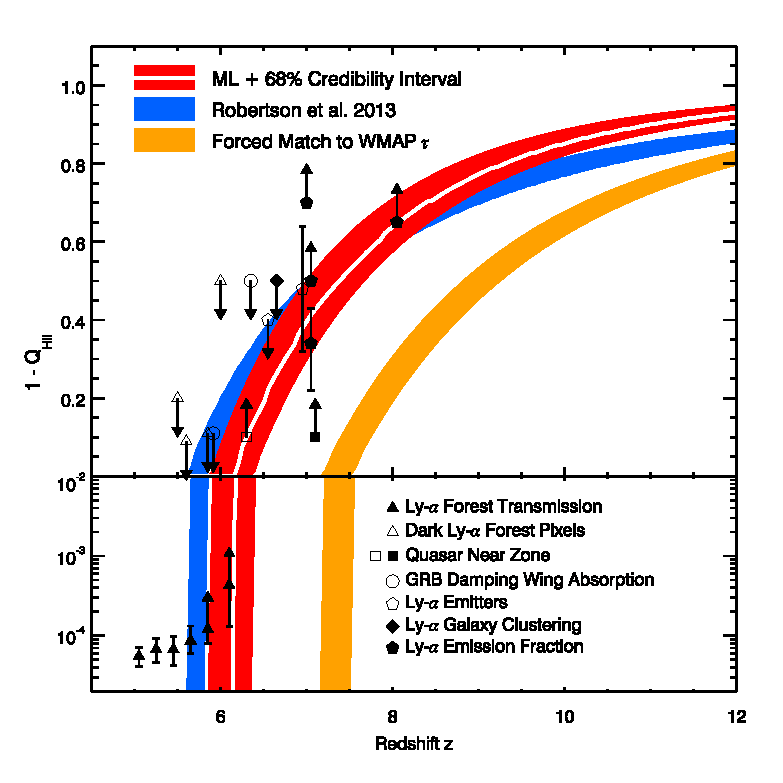
\includegraphics[width=12cm]{Robertson2015.eps}
  \caption{The above figure from \cite{robertson2015cosmic} overplots several claimed constraints on $\axhi$ during the Epoch of Reionization (markers), most of which we touch on in this section, along with best fit curves calculated using luminosity functions. The red shaded curve shows the maximum-likelihood model of the neutral fraction (white) with $1\sigma$ errors and is consistent with Planck $\tau_{\text{e}}$ measurements. The analogous curve for \cite{Robertson2013} is shown in blue, but is in conflict with the WMAP $\tau_{\text{e}}$ constraints. A model that forces the blue curve to satisfy the WMAP $\tau_{\text{e}}$ constraint is shown in yellow. This figure demonstrates that, under some assumptions, the scenario where galaxies dominate reionization is not in conflict with the constraints on the timing of the EoR to date.   }
  \label{fig:Robertson2015}
\end{figure}


\clearpage
\section{Moving Forward}


The previous section has serves in part to pay tribute to the extraordinary work that has gone into providing us with our current understanding of the Epoch of Reionization. However, it also demonstrates some of the challenges in interpreting previous measurements. Indeed, subtleties in interpreting quasar spectra have lead to the questionable conclusion that reionization has completed by $z \sim 6$, for example. Thus, this motivates the development of other techniques which, while invariably faced with their own difficulties, might circumvent these complications. Throughout the rest of this thesis, we will develop complementary measurement techniques to those mentioned thus far in hopes to expand our current understanding. 


In \S \ref{sec:NeutralIslands}, we propose two novel approaches for searching for signatures of underlying neutral hydrogen in the \lya\ and \lyb\ forest of distant quasars. We show that, if the Universe is $\gtrsim 5\%$ neutral at $z \sim 5.5$, then damping-wing absorption from neutral hydrogen and absorption from primordial deuterium should leave an observable imprint in the \lya\ and \lyb\ forest, respectively. Furthermore, the presence of neutral islands should qualitatively alter the size distribution of absorbed regions.


We continue in \S \ref{sec:IGMTemperature} by discussing the ability for the intergalactic medium to retain a thermal memory of the reionization process at redshifts $z \sim 5$ which in turn affects the small-scale structure in the \lya\ forest. Motivated by this, we model the temperature of the intergalactic medium after reionization and develop a temperature measurement technique that should be able to distinguish between  scenarios where reionization ends at $z \sim 6$ and at $z \sim 10$. 


Lastly, we turn our attention to 21-cm observations during reionization in \S \ref{sec:Bubble}. We demonstrate that, while precise mapping of 21-cm emission from neutral hydrogen should be infeasible by first and second generation interferometers, it may be possible to make \textit{crude} maps of the reionization process and identify individual ionized regions. This would provide us with direct confirmation that we are observing reionization and provide information as to its timing and the nature of the ionizing sources.
